\chapter{Исследование многообразия энергетически оптимальных решений задачи встречи в плоской круговой модели движения небесных тел}

% Микровведение к главе 2

В настоящей главе исследуется структура решений энергетически оптимальной задачи встречи в плоской круговой модели движения небесных тел. В качестве исходной мотивации рассматривается многоветвистая структура перелётов Земля--Марс в эфемеридной постановке, после чего выполняется переход к модельной задаче для виртуальных небесных тел на круговых компланарных орбитах. Далее показывается, что после устранения эфемеридной зависимости наблюдаемая структура переходит в односвязное модельное многообразие, на котором при дополнительном условии на свободный правый конец выделяется кривая локальных оптимумов. На этой кривой вводятся точки оптимальной дальности и строятся конечные формулы для продолжительности перелёта, нормированной непрерывной фазы, квадратичного функционала и параметров оптимального управления. Отдельно рассматривается область малой витковой дальности, необходимая для устойчивого использования полученных зависимостей при построении начальных приближений. В заключительной части главы приводится верификация качества конечных формул и проверка согласованности восстановленных решений с краевыми условиями.

\section{Мотивационный пример: семейства решений в эфемеридной задаче Земля--Марс}

Исследование, изложенное в настоящей главе, возникло из наблюдаемой структуры реальных межпланетных перелётов. Рассмотрим энергетически оптимальные перелёты Земля--Марс, рассчитанные в эфемеридной постановке. В этой задаче внешними параметрами выступают дата старта и угловая дальность, а в качестве характеристик решения естественно рассматривать продолжительность перелёта и значение функционала. Уже на этом уровне обнаруживается, что при одних и тех же внешних параметрах задача не сводится к единственной ветви решений.

\begin{figure}[htbp]
	\centering
	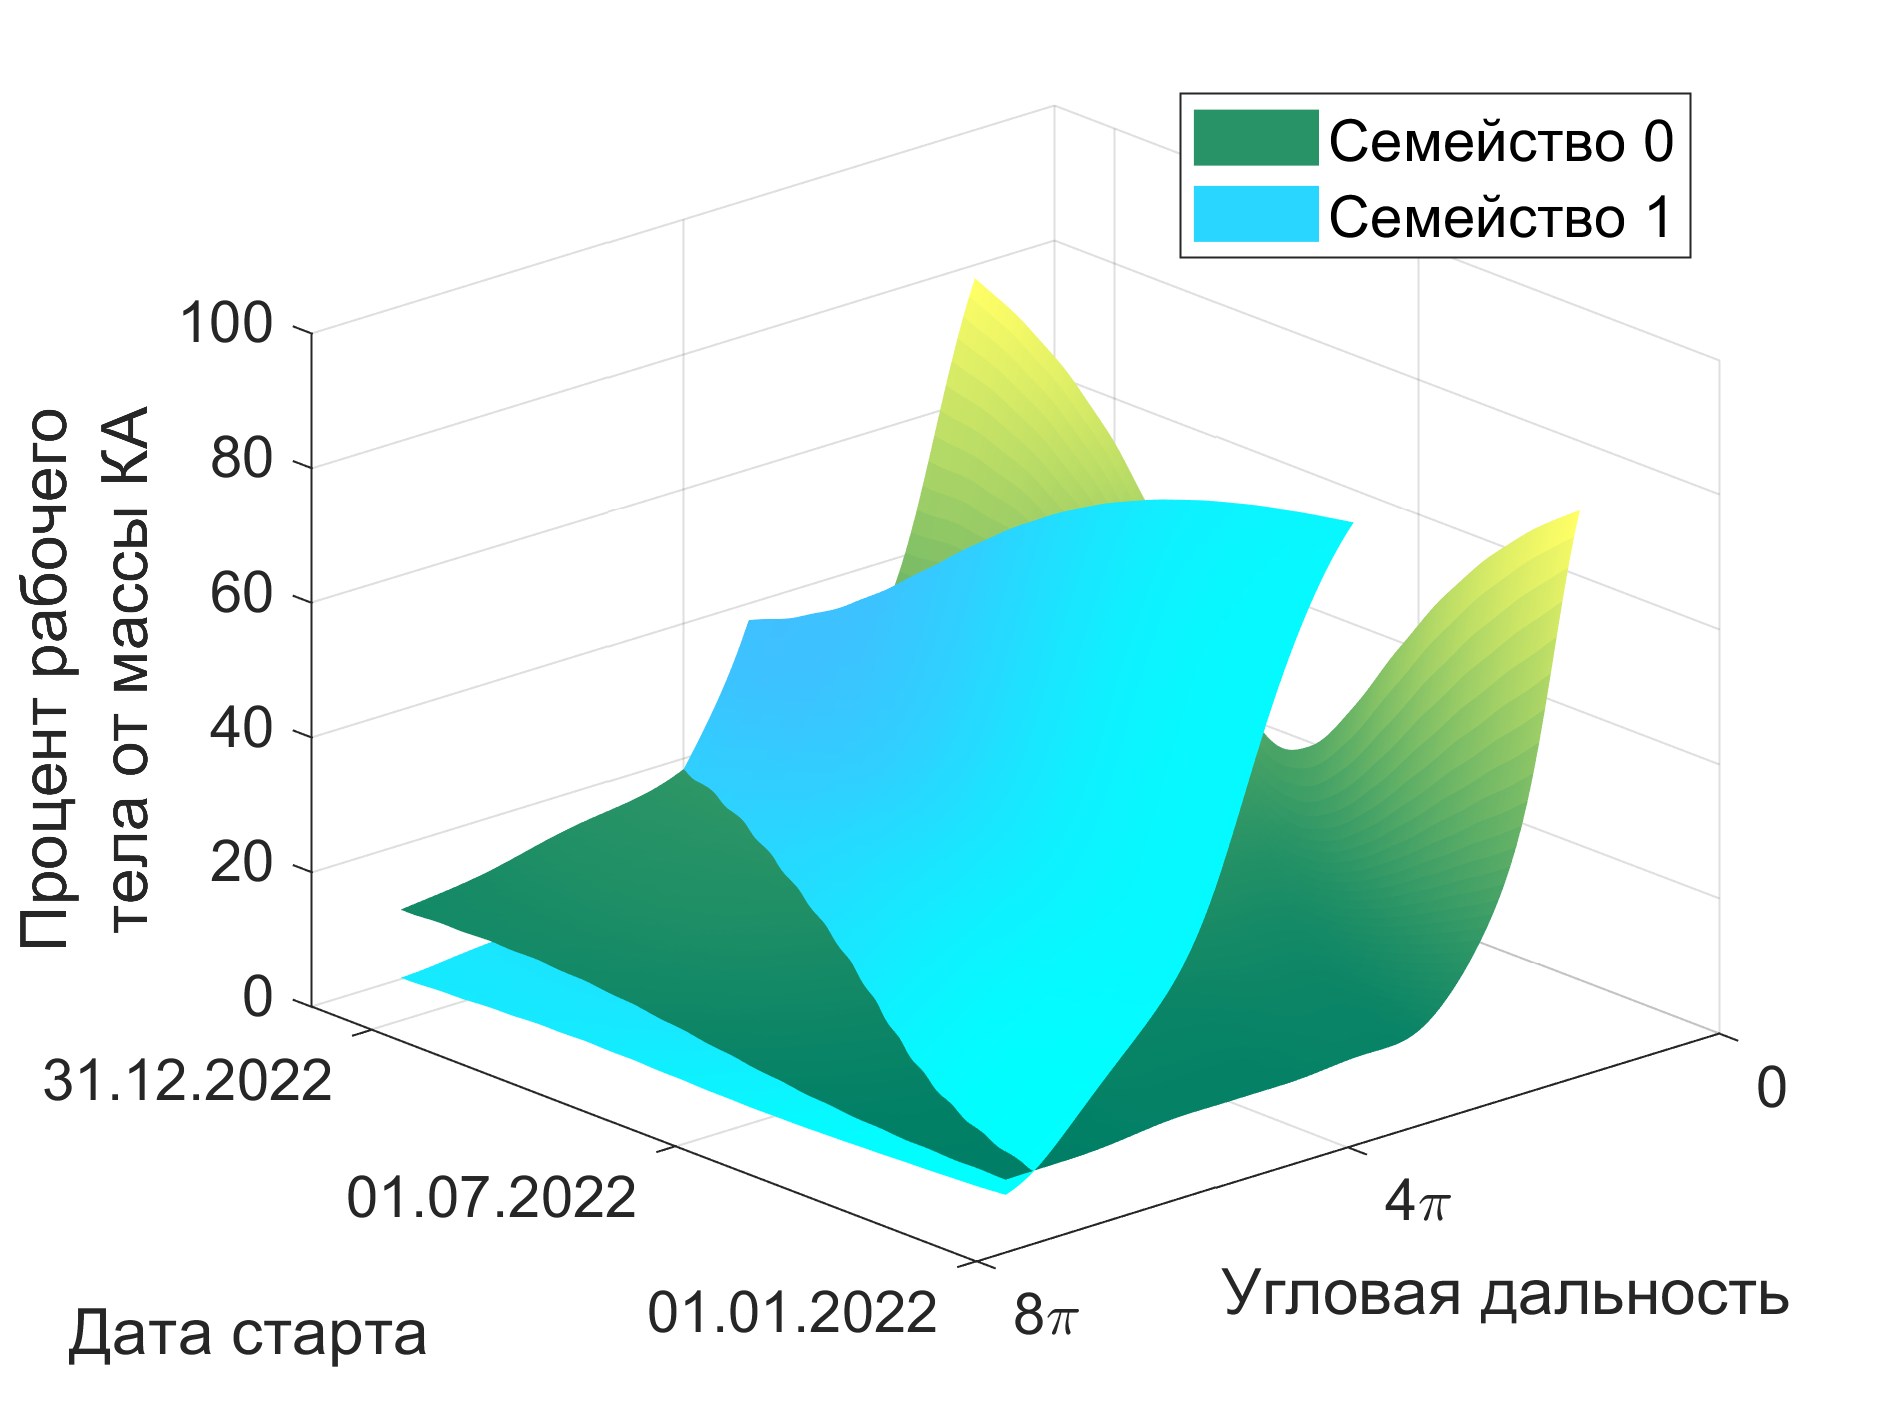
\includegraphics[width=0.82\textwidth]{images/Startdate.png}
	\caption{Структура энергетически оптимальных перелётов Земля--Марс в координатах дата старта -- угловая дальность}
	\label{fig:startdate_mars_families}
\end{figure}

На рис.~\ref{fig:startdate_mars_families} показан характерный пример такой структуры. По горизонтальной оси отложена дата старта, по вертикальной --- угловая дальность, а цветом представлено значение функционала. Видно, что множество решений распадается на несколько обособленных ветвей. Далее такие ветви будем называть \textit{семействами решений}. В данном разделе этот термин используется именно в мотивационном смысле: он описывает наблюдаемую структуру эфемеридной задачи и не вводится как основной термин для модельной части главы.

Возникновение семейств решений в этом примере связано с тем, что перелёты, близкие по геометрии, могут различаться по числу дополнительных оборотов и, как следствие, по продолжительности перелёта и значению функционала. При этом в эфемеридной постановке такие семейства технически остаются различными. Даже если рассматривать сдвиг на синодический период, конфигурация реальных планет не воспроизводится тождественно, поскольку движение задаётся эфемеридами, а не кеплеровской моделью. Поэтому наблюдаемая многоветвистая структура не сводится к простой периодической повторяемости.

Именно этот факт служит отправной мотивацией дальнейшего анализа. С одной стороны, исходный график имеет непосредственный прикладной смысл: дата старта является физической величиной, а выявляемые на нём окна перелёта наблюдаемы и важны для баллистического проектирования. С другой стороны, сама структура графика оказывается слишком сложной для прямого исследования и тем более для построения компактных аналитических зависимостей. Это приводит к необходимости перейти к упрощённой постановке, в которой календарная дата старта заменяется начальной синодической фазой, а реальные планеты --- виртуальными небесными телами на круговых компланарных орбитах.

Таким образом, дальнейший переход к модельной постановке не является искусственным упрощением ради удобства вычислений. Напротив, он представляет собой способ выделить и исследовать в чистом виде ту же самую структурную особенность, которая впервые проявилась в эфемеридной задаче Земля--Марс, а именно многоветвистость множества энергетически оптимальных решений. В следующем разделе будет показано, что после устранения эфемеридной зависимости эта структура естественным образом переходит в односвязное модельное многообразие, которое в разных координатных представлениях может выглядеть по-разному.


\section{Переход к модельной постановке и геометрия односвязного модельного многообразия}

Наблюдаемая в эфемеридной задаче многоветвистая структура решений требует более простой постановки, в которой основные геометрические закономерности можно исследовать независимо от календарных и эфемеридных особенностей конкретной миссии. Кроме этого, для уменьшения числа независимых параметров, таких как наклонение и эксцентриситет, ограничимся компланарными круговыми орбитами. Для этого перейдём от реальных планет к виртуальным небесным телам, движущимся по круговым компланарным орбитам, и заменим дату старта начальной синодической фазой. 

В рассматриваемой модельной задаче фиксируются начальные граничные условия, соответствующие движению по круговой орбите единичного радиуса, а конечные граничные условия задаются отношением радиусов $\kappa$ и угловой дальностью $\varphi$. Для дальнейшего анализа удобно перейти от угловой дальности к витковой дальности
\begin{equation}
	\lambda = \frac{\varphi}{2\pi},
\end{equation}
поскольку именно параметр $\lambda$ естественно отражает многовитковый характер решений. Таким образом, при фиксированном значении $\kappa$ множество решений можно рассматривать как геометрический объект в пространстве параметров, включающем начальную синодическую фазу, витковую дальность, продолжительность перелёта и значение функционала.
\begin{equation}
	\mathbf c=\left(\Phi,\lambda,T, J \right).
\end{equation}

\begin{figure}[htbp]
	\centering
	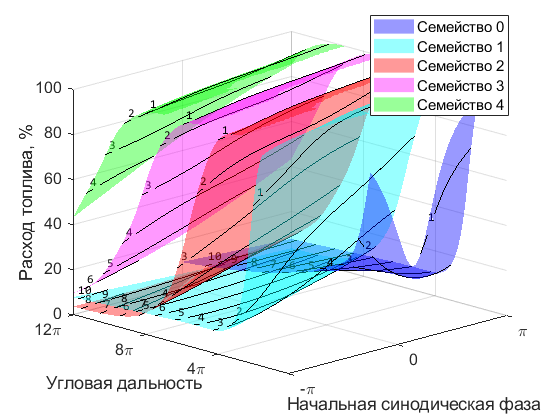
\includegraphics[width=0.82\textwidth]{images/5families.png}
	\caption{Одно из представлений модельного многообразия в координатах начальная синодическая фаза -- витковая дальность}
	\label{fig:chap2_5families}
\end{figure}

На рис.~\ref{fig:chap2_5families} показано одно из таких представлений. В координатах начальная синодическая фаза -- витковая дальность одно и то же множество решений визуально распадается на несколько ветвей. Это представление связано с рис.~\ref{fig:startdate_mars_families}, поскольку начальная синодическая фаза является аналогом даты старта. Однако в модельной постановке визуальный распад на несколько семейств зависит от выбора координат и отражает способ представления многообразия, а не наличие нескольких независимых множеств решений.

Для выявления внутренней геометрии объекта удобнее использовать другое координатное представление, в котором вместо начальной синодической фазы рассматривается продолжительность перелёта. При таком переходе те же самые решения образуют односвязное модельное многообразие.

\begin{figure}[htbp]
	\centering
	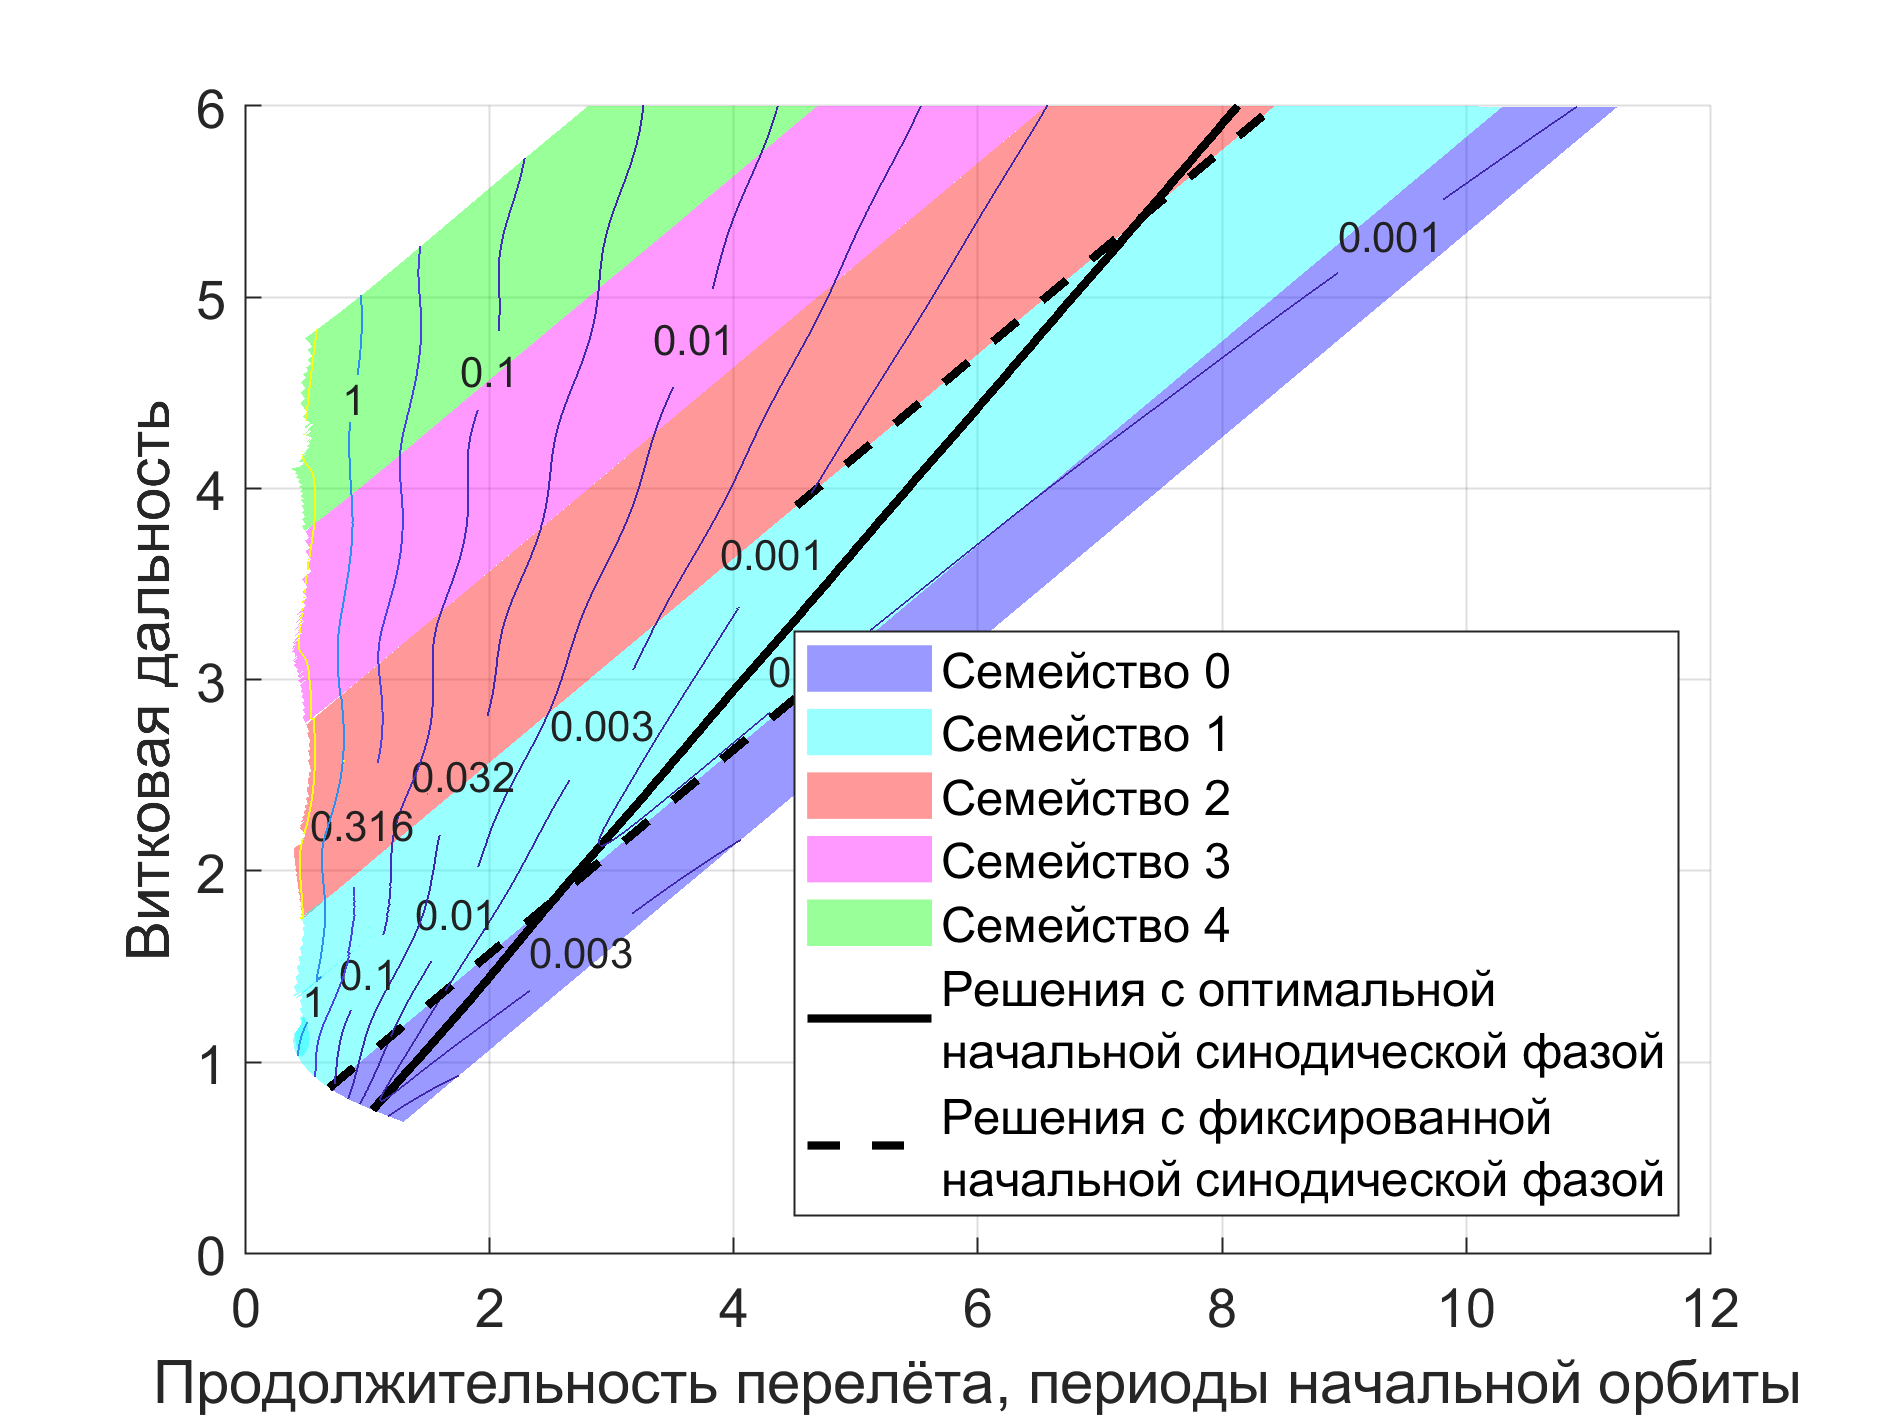
\includegraphics[width=0.78\textwidth]{images/UnitedManifold.png}
	\caption{Односвязное модельное многообразие в координатах продолжительность перелёта -- витковая дальность}
	\label{fig:chap2_united_manifold}
\end{figure}

На рис.~\ref{fig:chap2_united_manifold} видно, что после замены координат ранее наблюдавшиеся ветви сливаются в односвязное модельное многообразие. Тем самым семейства решений, введённые в мотивационном разделе, оказываются не базовой структурой модельной задачи, а координатно-зависимым способом видеть один и тот же объект.

Переход к модельной постановке тем самым решает две задачи. Во-первых, он устраняет эфемеридную зависимость и позволяет исследовать структуру решений в чистом виде. Во-вторых, он даёт возможность перейти от календарно заданной прикладной задачи к геометрическому описанию, в котором далее можно выделить специальное подмногообразие локально оптимальных решений. В следующем разделе для односвязного модельного многообразия будет введена кривая локальных оптимумов.


\section{Кривая локальных оптимумов}

При анализе односвязного модельного многообразия в координатах продолжительность перелёта -- витковая дальность обнаруживается важная закономерность: в исследованной области параметров при фиксированных значениях $\kappa$ и $T$ функционал имеет одно локально минимальное значение по витковой дальности. Наблюдение именно этой структуры и приводит к введению кривой локальных оптимумов. Таким образом, речь идёт не о формальном выделении произвольного подмногообразия, а о специальной ветви решений, существование которой непосредственно следует из численно наблюдаемой геометрии модельного многообразия.

Для локально оптимального значения витковой дальности далее используется обозначение
\begin{equation}
	J\left(T,\lambda^\star,\kappa\right)=\min_{\lambda} J\left(T,\lambda,\kappa\right),
\end{equation}
где $\lambda^\star$ обозначает локально оптимальное значение витковой дальности при фиксированных $T$ и $\kappa$. Совокупность таких значений образует одномерное подмногообразие модельного многообразия, которое далее будем называть \textit{кривой локальных оптимумов}.

Переход от двумерного модельного многообразия к кривой локальных оптимумов осуществляется не отбором точек на ранее построенной координатной сетке. Численно к модельному многообразию применяется дополнительное условие на свободный правый конец согласно принципу максимума, после чего выполняется продолжение решения уже для новой постановки. Тем самым кривая локальных оптимумов строится как новая ветвь решений, а не как результат постобработки заранее рассчитанного массива точек.

\begin{figure}[htbp]
	\centering
	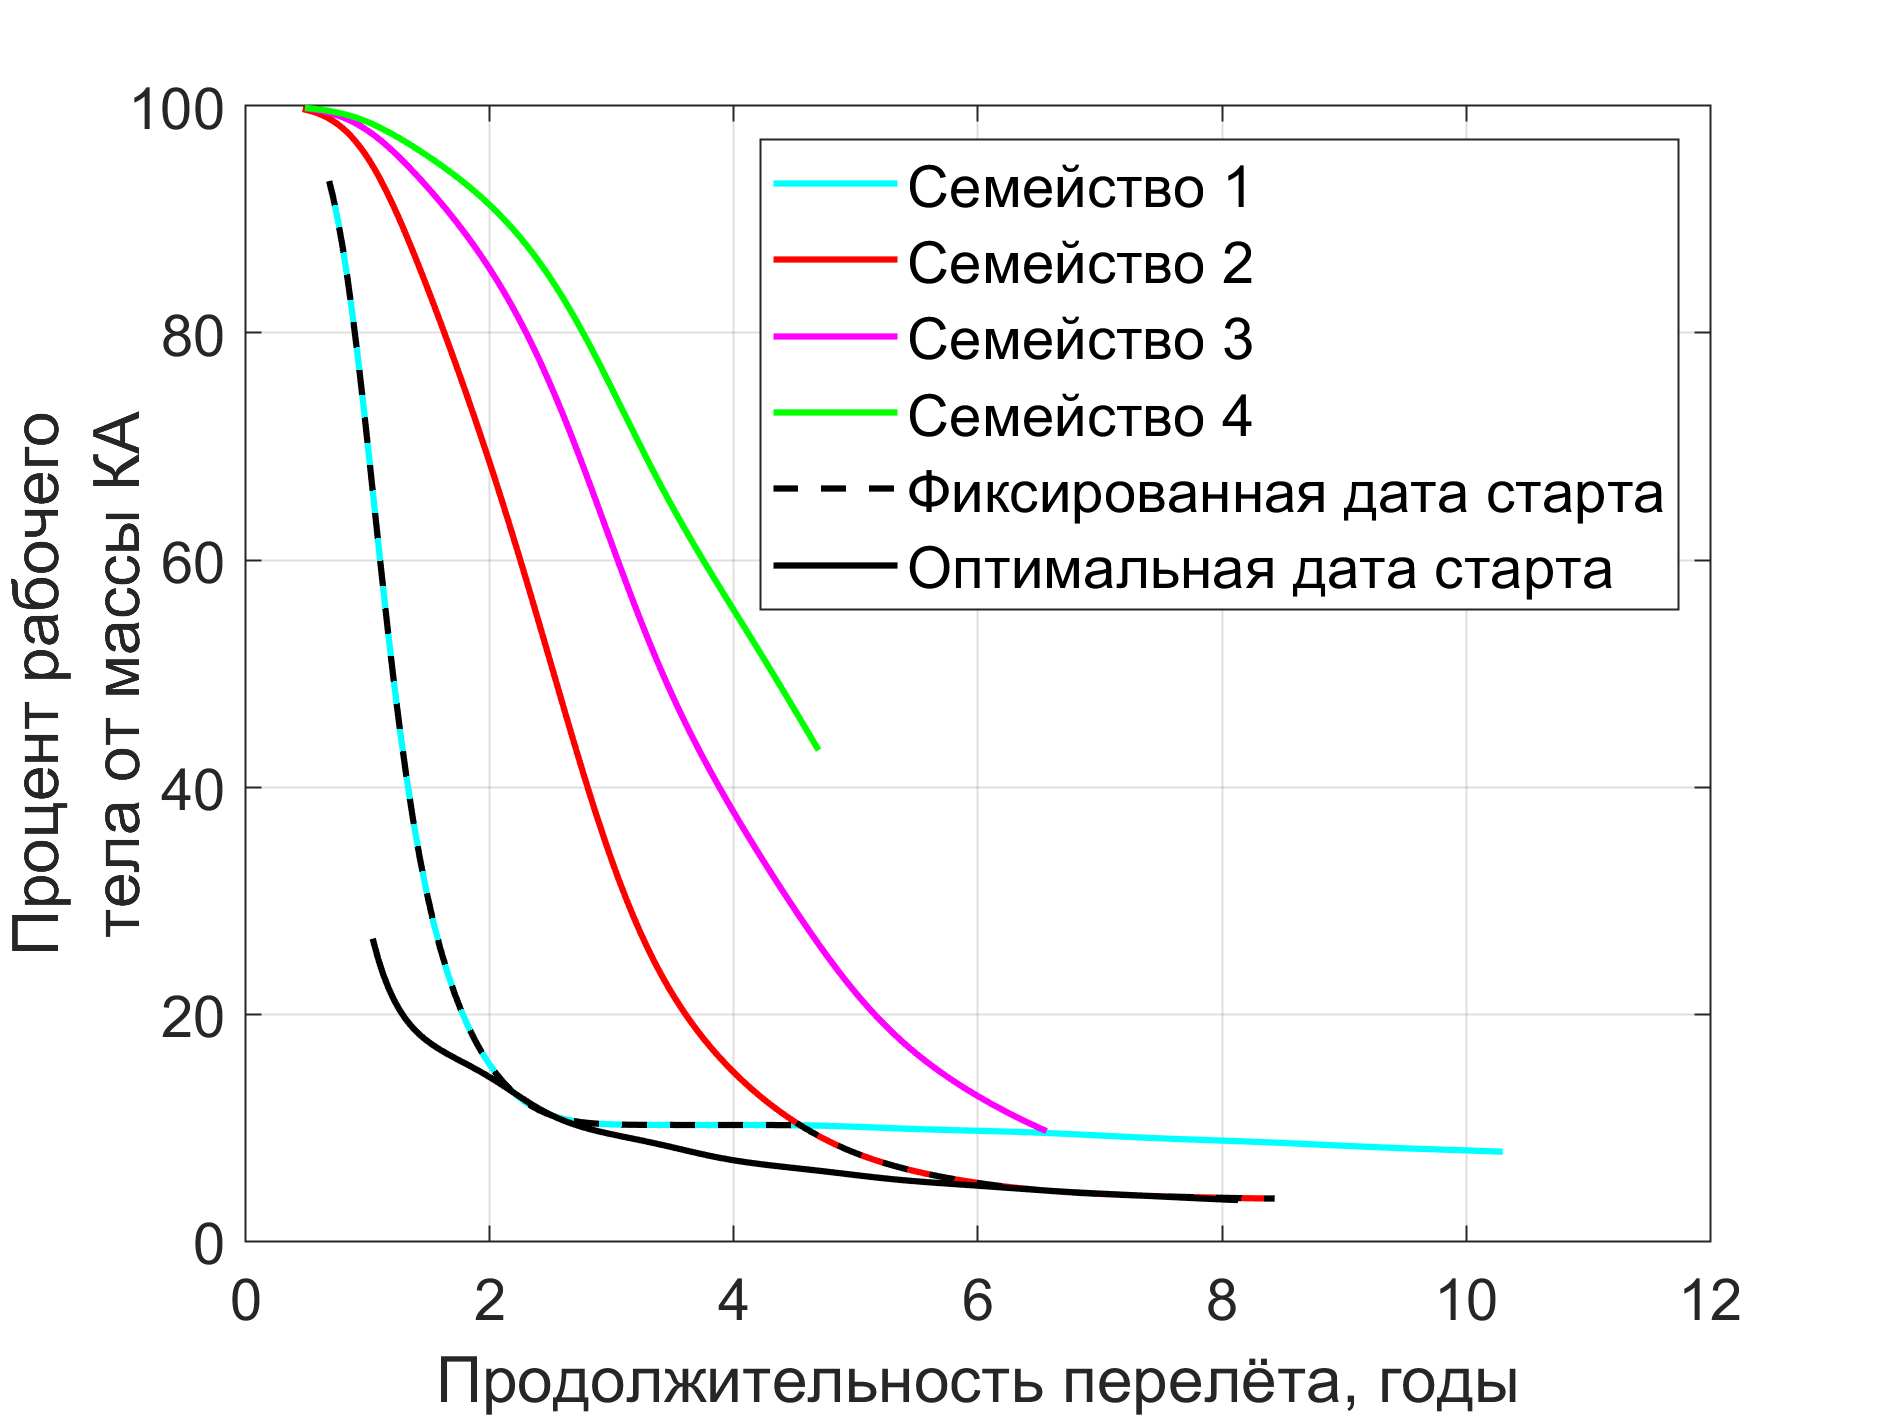
\includegraphics[width=0.78\textwidth]{images/ParetoToF.png}
	\caption{Кривая локальных оптимумов в координатах продолжительность перелёта -- витковая дальность}
	\label{fig:chap2_pareto_tof}
\end{figure}

На рис.~\ref{fig:chap2_pareto_tof} показана кривая локальных оптимумов для фиксированного значения $\kappa$. Именно на этом этапе происходит сужение от двумерного модельного многообразия к одномерной структуре, которая далее служит основой для построения конечных формул. Для случая $\kappa=1.52$, соответствующего перелёту типа Земля--Марс, уже на раннем этапе исследования была отмечена простая линейная аппроксимация этой кривой \cite{korneev_duration_ngpm_2024}:
\begin{equation}
	\widehat{T} \approx 1.35 + 0.0394\,\lambda^\star .
\end{equation}
Хотя в дальнейшем используются более точные конечные формулы, сама возможность такой простой аппроксимации хорошо отражает регулярный характер кривой локальных оптимумов.

Кривая локальных оптимумов играет в дальнейшем принципиальную роль. Во-первых, именно на ней будут построены конечные формулы для продолжительности перелёта, начальной синодической фазы, квадратичного функционала и параметров оптимального управления. Во-вторых, в координатах начальная синодическая фаза -- витковая дальность она допускает естественную интерпретацию через пересечения с изолиниями фиксированной начальной синодической фазы. Эти пересечения образуют счётное множество точек, которое будет рассмотрено в следующем разделе.


\section{Точки оптимальной дальности}

Кривая локальных оптимумов задаёт локально оптимальные значения витковой дальности при фиксированных продолжительности перелёта и отношении радиусов. Однако в прикладной задаче обычно фиксируется не продолжительность перелёта, а дата старта. В модельной постановке её геометрическим аналогом является начальная синодическая фаза. Поэтому следующим шагом необходимо рассмотреть пересечения кривой локальных оптимумов с изолиниями фиксированной начальной синодической фазы.

\begin{figure}[htbp]
	\centering
	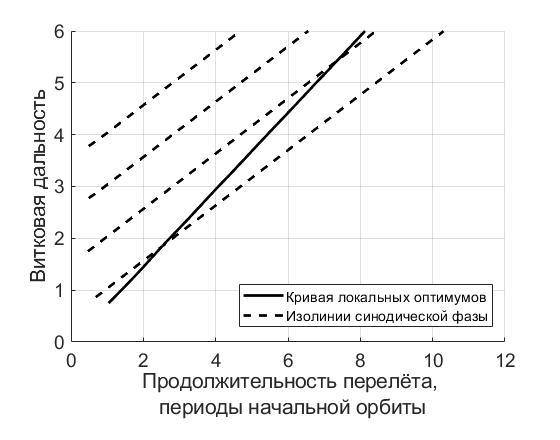
\includegraphics[width=0.78\textwidth]{images/Isolines.png}
	\caption{Точки оптимальной дальности как пересечения кривой локальных оптимумов с изолиниями фиксированной начальной синодической фазы}
	\label{fig:chap2_optimal_distance_points}
\end{figure}

\textit{Точки оптимальной дальности} --- это счётное множество точек пересечения кривой локальных оптимумов с изолиниями фиксированной начальной синодической фазы. Каждая такая точка соответствует локально оптимальному значению витковой дальности при заданной дате старта.

На рис.~\ref{fig:chap2_optimal_distance_points} показана геометрическая интерпретация этого определения. Кривая локальных оптимумов задаёт допустимые локально оптимальные значения витковой дальности, а изолинии начальной синодической фазы выделяют из неё те решения, которые соответствуют выбранной дате старта. В результате для одной и той же даты может существовать не одна, а несколько точек оптимальной дальности.

Важно подчеркнуть, что точки оптимальной дальности определены только после фиксации начальной синодической фазы. При изменении даты старта соответствующие изолинии сдвигаются, а вместе с ними сдвигаются и точки пересечения с кривой локальных оптимумов. При этом отдельные точки могут выходить из физически допустимой области $T>0$, а новые точки, наоборот, входить в неё. Поэтому простая нумерация точек по положению на графике не является устойчивой.

При построении конечных формул возникает дополнительная техническая трудность. Начальная синодическая фаза является геометрической величиной, заданной с точностью до периода, поэтому при приведении к основному диапазону она имеет разрывы. Непосредственная аппроксимация такой разрывной зависимости затруднительна. Поэтому далее вместо неё используется нормированная непрерывная фаза, то есть развёртка синодической фазы по витковой дальности.

\begin{figure}[htbp]
	\centering
	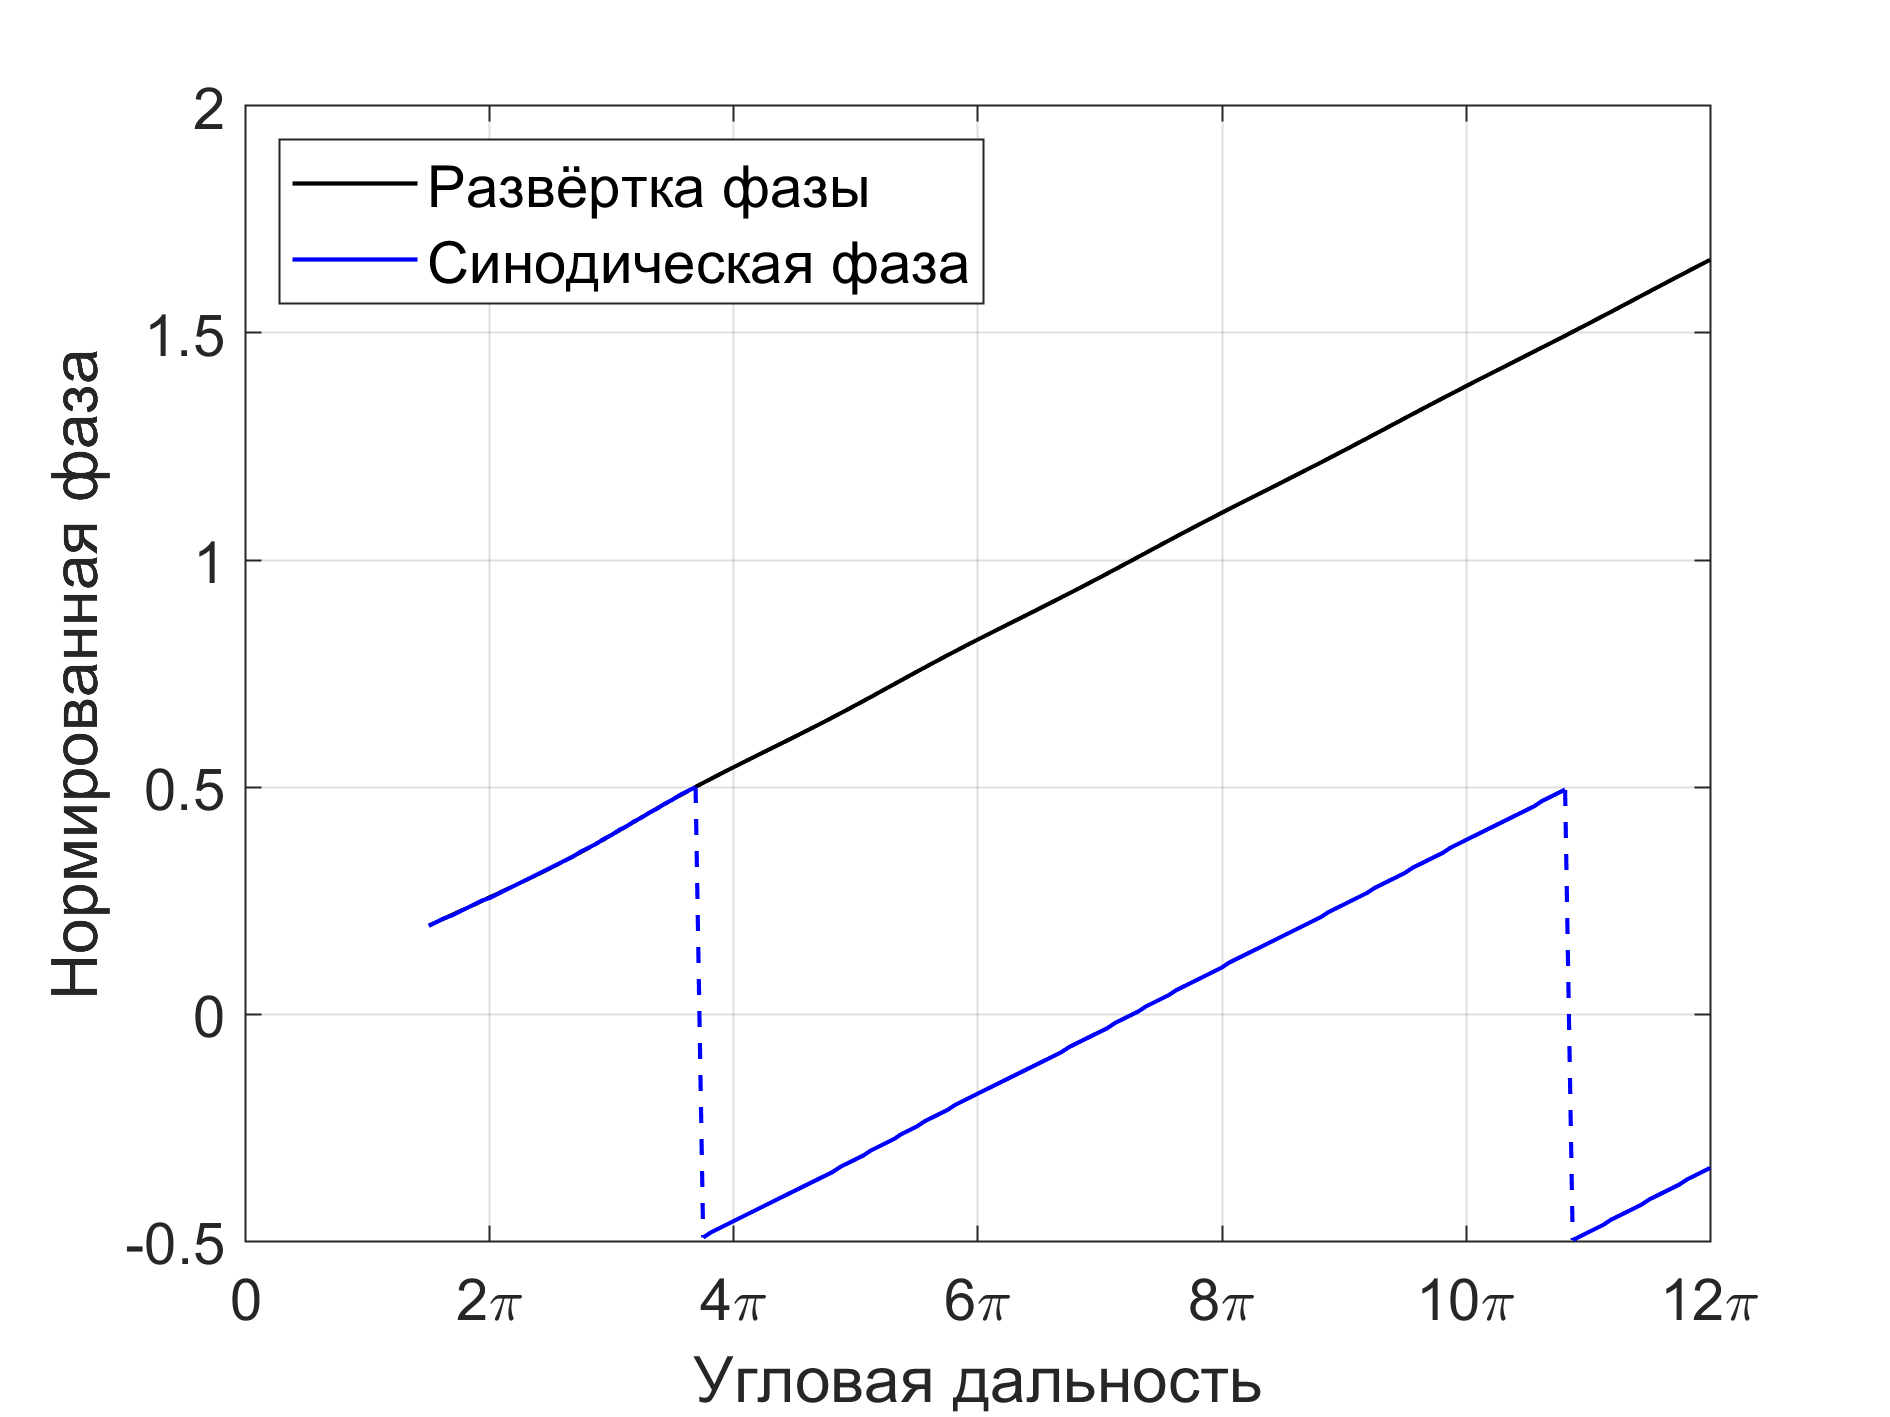
\includegraphics[width=0.78\textwidth]{images/PhaseLongitude.png}
	\caption{Связь между синодической фазой и её непрерывной развёрткой}
	\label{fig:chap2_phase_longitude}
\end{figure}

На рис.~\ref{fig:chap2_phase_longitude} показана эта связь. Синодическая фаза после приведения к основному диапазону имеет скачки, тогда как её развёртка изменяется непрерывно. Введём обозначение $\Psi$ для нормированной непрерывной фазы. Если $\Phi$ обозначает начальную синодическую фазу в радианной мере, то значение $\Phi/(2\pi)$ задаёт нормированную фазу с точностью до целого числа оборотов. Непрерывная фаза $\Psi$ выбирает одну из таких ветвей и тем самым устраняет разрывы, мешающие аппроксимации.

Таким образом, точки оптимальной дальности связывают геометрическое описание кривой локальных оптимумов с прикладной постановкой, в которой задаётся дата старта. При фиксированной начальной синодической фазе они выделяют на кривой локальных оптимумов те значения витковой дальности, которые соответствуют выбранной конфигурации тел. При этом для последующего построения конечных формул удобнее работать не с разрывной синодической фазой, а с её нормированной непрерывной развёрткой $\Psi$. Это позволяет сохранить геометрический смысл начальной синодической фазы и одновременно получить гладкую зависимость, пригодную для аппроксимации.


\section{Конечные формулы для продолжительности перелёта, непрерывной фазы и квадратичного функционала}

После выделения кривой локальных оптимумов и введения точек оптимальной дальности следующей задачей становится получение компактных конечных формул для основных характеристик перелёта. В данном разделе рассматриваются конечные формулы для продолжительности перелёта, нормированной непрерывной фазы и квадратичного функционала. Эти величины определяют положение решения на кривой локальных оптимумов и позволяют восстановить основные баллистические характеристики перелёта без повторного решения двухточечной краевой задачи.

Далее будем различать кинематические связи, следующие из постановки задачи и введённых обозначений, и конечные формулы, полученные методом символьной регрессии. Для конечных формул используется знак крышки. Так, $\widehat{T}$, $\widehat{\Psi}$ и $\widehat{J}$ обозначают конечные формулы для продолжительности перелёта, нормированной непрерывной фазы и квадратичного функционала соответственно. Точность этих формул будет далее охарактеризована среднеквадратической ошибкой на тестовой выборке.

Для продолжительности перелёта используется конечная формула
\begin{equation}
	\widehat{T}\left(\lambda^\star,\kappa\right)=
	\frac{2}{27}\kappa\ln\kappa
	+
	\lambda^\star
	\left(
	\kappa-\frac{\sqrt6}{9}\kappa\ln\kappa
	\right).
\end{equation}
Здесь независимыми переменными являются локально оптимальная витковая дальность $\lambda^\star$ и отношение радиусов $\kappa$. Формула сохраняет правильное поведение в предельном случае совпадающих круговых орбит:
\begin{equation}
	\widehat{T}\left(\lambda^\star,1\right)=\lambda^\star .
\end{equation}
Тем самым конечная формула для продолжительности перелёта не только описывает численно построенную кривую локальных оптимумов, но и согласуется с простейшим предельным режимом пассивного движения.

\begin{figure}[htbp]
	\centering
	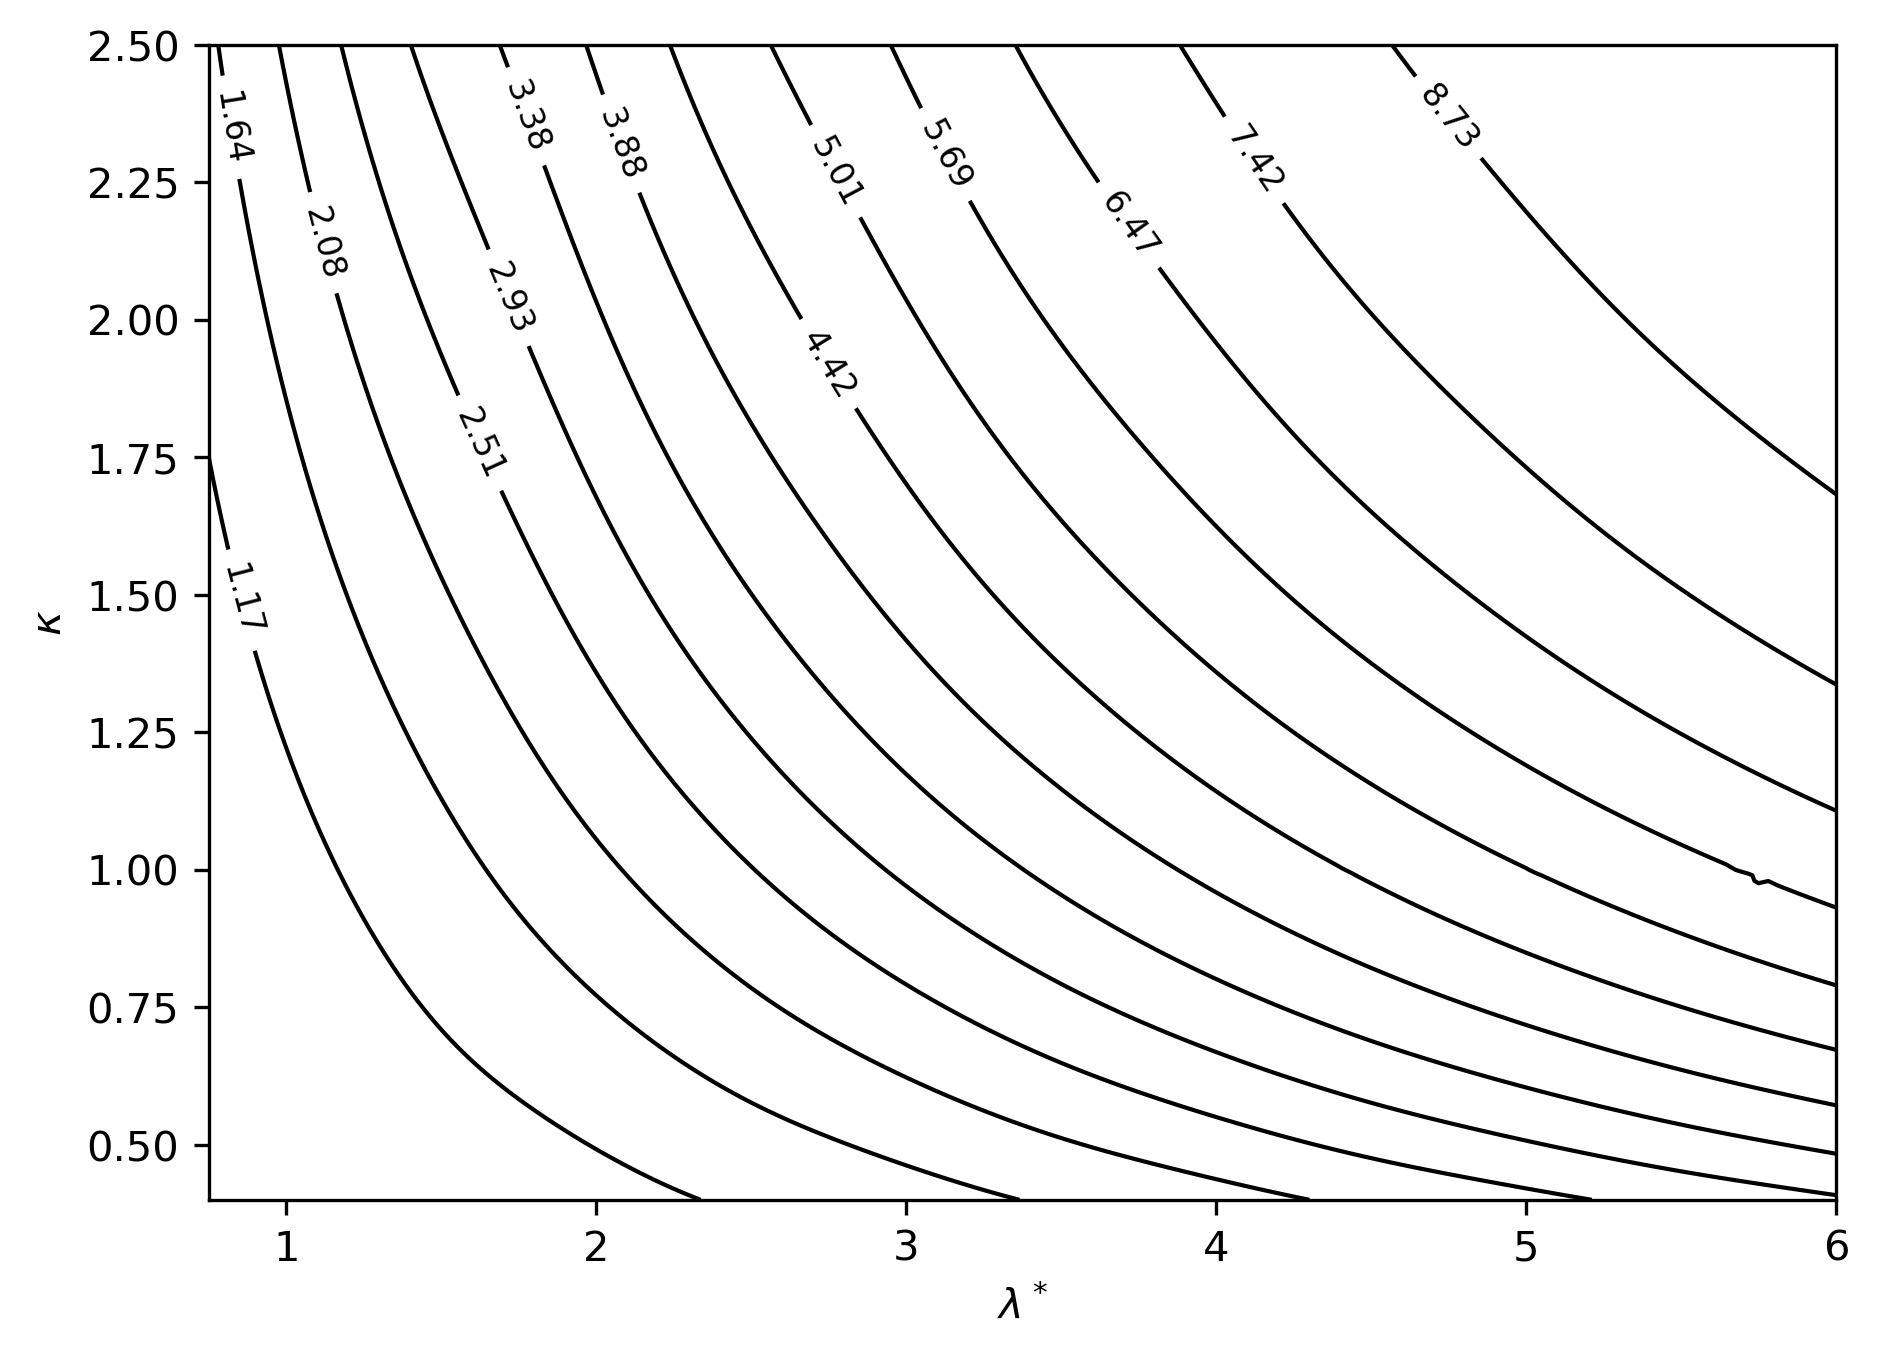
\includegraphics[width=0.82\textwidth]{images/main_T_isolines.png}
	\caption{Изолинии продолжительности перелёта на основной области}
	\label{fig:chap2_main_t_isolines}
\end{figure}

На рис.~\ref{fig:chap2_main_t_isolines} показана структура продолжительности перелёта в координатах $\lambda^\star$ и $\kappa$. Изолинии отражают гладкий характер зависимости, что согласуется с простым видом конечной формулы для $\widehat{T}$.

Между продолжительностью перелёта, витковой дальностью и непрерывной фазой существует кинематическая связь. В используемой нормировке её можно записать в виде
\begin{equation}
	\Psi =
	\lambda^\star-\frac{T}{\kappa^{3/2}}.
\end{equation}
Поэтому после получения конечной формулы для продолжительности перелёта можно построить производную оценку непрерывной фазы:
\begin{equation}
	\widehat{\Psi}_{T}\left(\lambda^\star,\kappa\right)
	=
	\lambda^\star-\frac{\widehat{T}\left(\lambda^\star,\kappa\right)}{\kappa^{3/2}}.
\end{equation}
Подставляя сюда конечную формулу для $\widehat{T}$, получаем
\begin{equation}
	\widehat{\Psi}_{T}\left(\lambda^\star,\kappa\right)=
	\left(
	1-\frac{1}{\sqrt{\kappa}}
	+\frac{\sqrt6}{9}\frac{\ln\kappa}{\sqrt{\kappa}}
	\right)\lambda^\star
	-
	\frac{2}{27}\frac{\ln\kappa}{\sqrt{\kappa}}.
\end{equation}

Таким образом, непрерывная фаза может быть восстановлена двумя способами: через кинематическую связь с продолжительностью перелёта или с помощью самостоятельной конечной формулы, полученной методом символьной регрессии. Далее используется самостоятельная формула для $\widehat{\Psi}$, а качество обоих вариантов будет сопоставлено при верификации конечных формул.

Как было отмечено в предыдущем разделе, непосредственная аппроксимация начальной синодической фазы затруднительна из-за её разрывов при приведении к основному диапазону. Поэтому для построения конечной формулы используется нормированная непрерывная фаза $\Psi$, представляющая собой развёртку синодической фазы по витковой дальности. Для кривой локальных оптимумов она записывается в виде
\begin{equation}
	\widehat{\Psi}\left(\lambda^\star,\kappa\right)
	=
	C^\Psi_0(\kappa)+C^\Psi_1(\kappa)\lambda^\star .
\end{equation}
Коэффициенты этой линейной зависимости являются функциями отношения радиусов:
\begin{equation}
	C^\Psi_0(\kappa)=-B e^{-\kappa}\ln^2\kappa,
\end{equation}
\begin{equation}
	C^\Psi_1(\kappa)=B\left(e^\kappa+1\right)e^{-\kappa}\ln\kappa,
\end{equation}
где
\begin{equation}
	B=0.543328.
\end{equation}
Таким образом, при фиксированном значении $\kappa$ непрерывная фаза описывается линейной функцией локально оптимальной витковой дальности, а зависимость от отношения радиусов полностью сосредоточена в коэффициентах $C^\Psi_0(\kappa)$ и $C^\Psi_1(\kappa)$.

\begin{figure}[htbp]
	\centering
	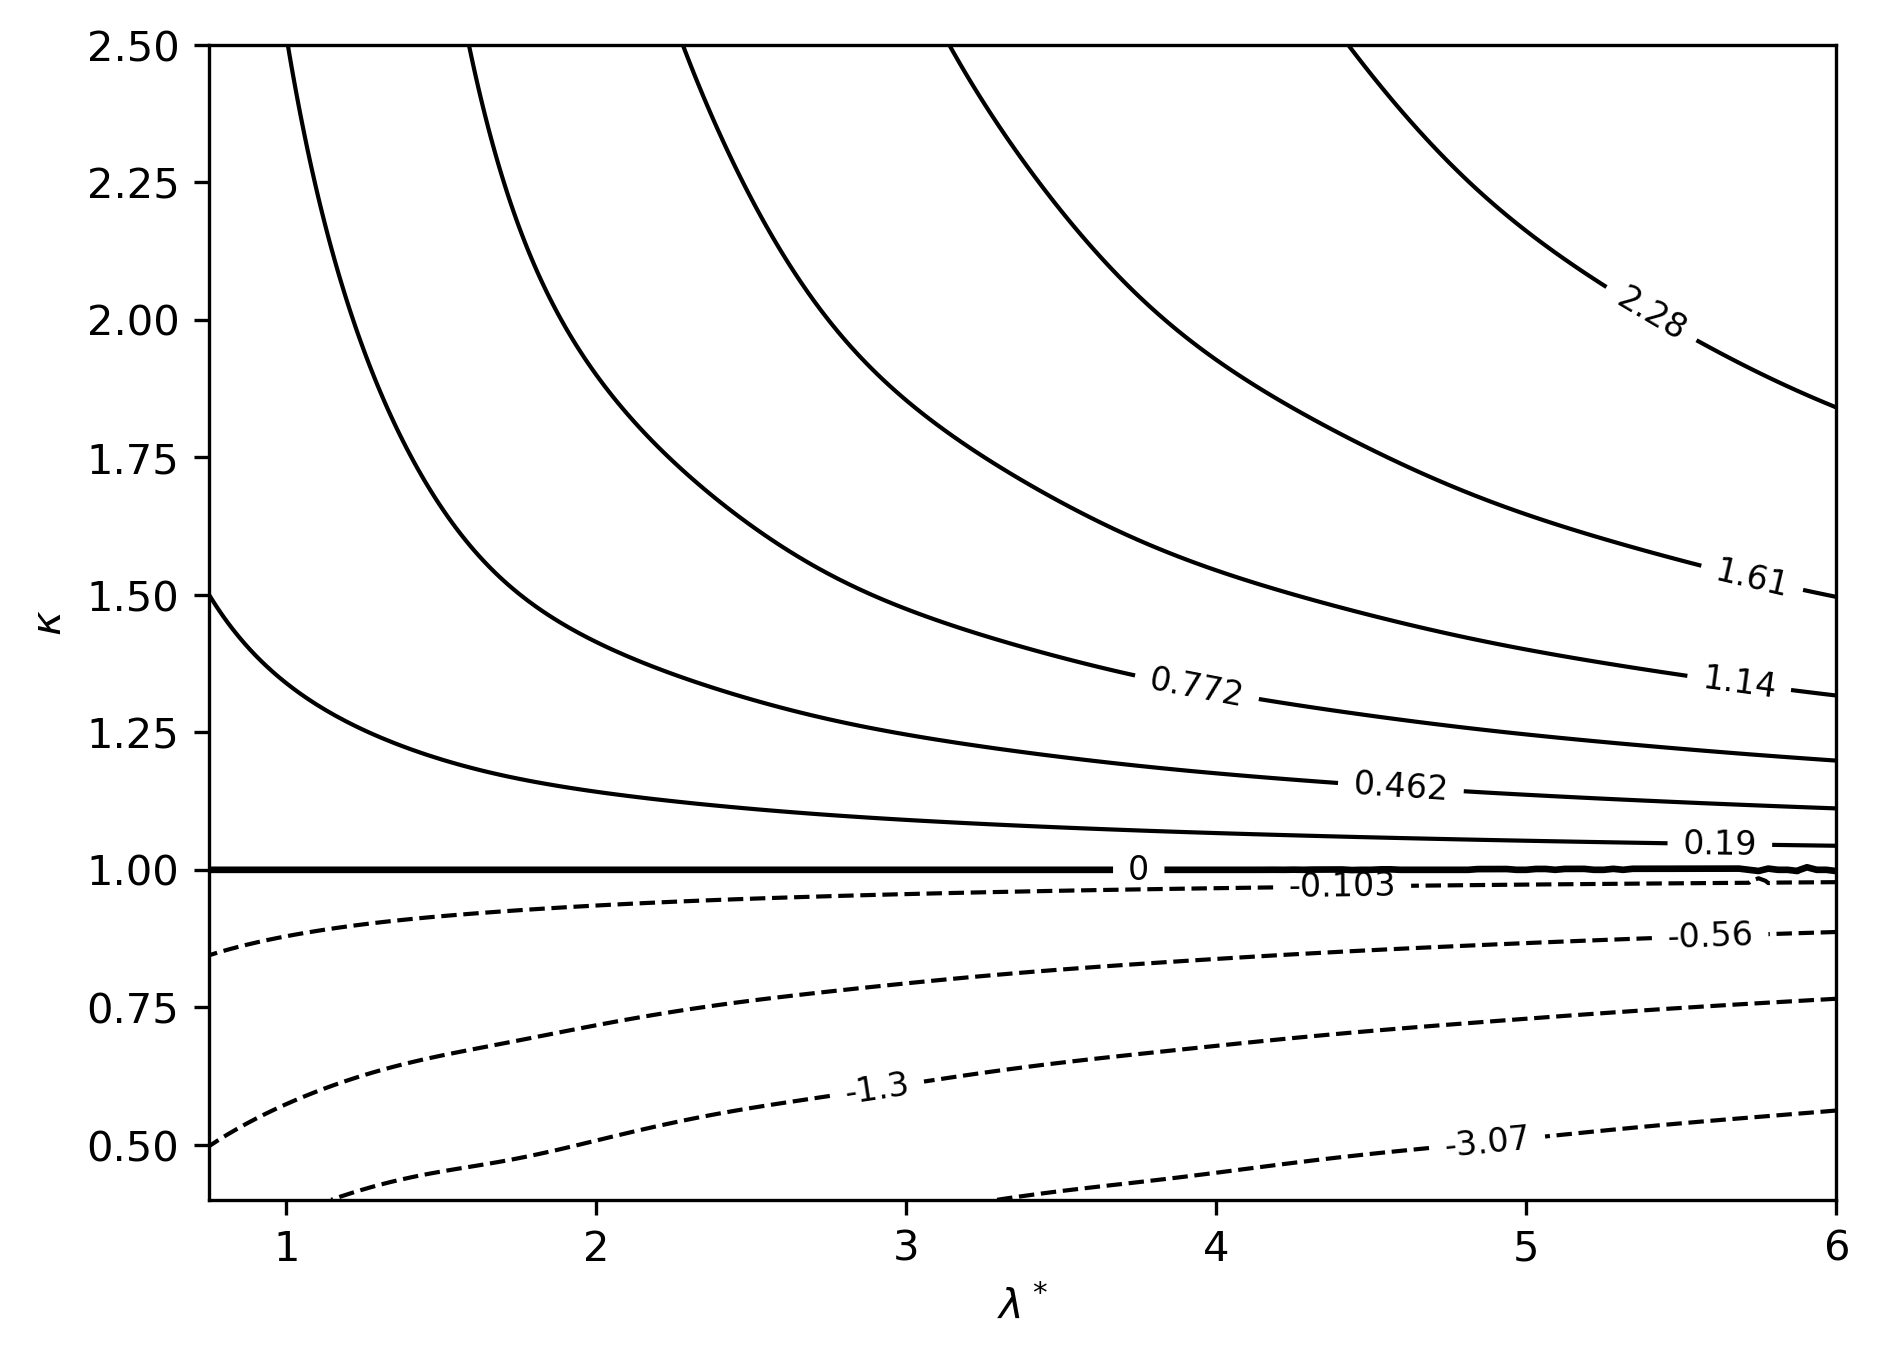
\includegraphics[width=0.82\textwidth]{images/main_phase_isolines.png}
	\caption{Изолинии нормированной непрерывной фазы на основной области}
	\label{fig:chap2_main_phase_isolines}
\end{figure}

На рис.~\ref{fig:chap2_main_phase_isolines} показана структура нормированной непрерывной фазы в координатах $\lambda^\star$ и $\kappa$. Использование развёртки позволяет заменить разрывную зависимость начальной синодической фазы гладкой функцией, пригодной для построения конечной формулы.

Эта формула позволяет перейти от заданной даты старта к точкам оптимальной дальности. Пусть для даты старта $t_0$ вычислена начальная синодическая фаза $\Phi(t_0)$. Тогда соответствующее нормированное значение фазы равно
\begin{equation}
	\Psi_0=\frac{\Phi(t_0)}{2\pi}.
\end{equation}
Поскольку непрерывная фаза разворачивает синодическую фазу по целому числу оборотов, точки оптимальной дальности находятся из условия
\begin{equation}
	\widehat{\Psi}\left(\widehat{\lambda}^{\star}_{k},\kappa\right)
	=
	\Psi_0+k,
	\qquad
	k=0,\pm1,\pm2,\ldots .
\end{equation}
Отсюда следует обратная формула для локально оптимальной витковой дальности:
\begin{equation}
	\widehat{\lambda}^{\star}_{k}
	=
	\frac{\Psi_0-C^\Psi_0(\kappa)+k}{C^\Psi_1(\kappa)},
	\qquad
	k=0,\pm1,\pm2,\ldots .
\end{equation}
Из полученного счётного множества далее рассматриваются только те значения $\widehat{\lambda}^{\star}_{k}$, которые попадают в физически допустимую область и область применимости конечных формул.

После определения $\widehat{\lambda}^{\star}_{k}$ продолжительность соответствующего перелёта вычисляется подстановкой этого значения в конечную формулу для продолжительности:
\begin{equation}
	\widehat{T}_k=
	\widehat{T}\left(\widehat{\lambda}^{\star}_{k},\kappa\right).
\end{equation}
Тем самым заданная дата старта порождает набор точек оптимальной дальности и соответствующий набор продолжительностей перелёта.

Для оценки энергетической цены перелёта используется конечная формула для квадратичного функционала:
\begin{equation}
	\widehat{J}\left(\lambda^\star,\kappa\right)=
	\frac{
		\left(
		C_0^J+\dfrac{C_1^J}{\kappa}+\dfrac{C_2^J}{\kappa^2}
		\right)\ln\kappa
	}{
		\lambda^\star
		+
		C_3^J
		\left(
		\sin\left(2\pi\lambda^\star+C_4^J-\frac{1}{\lambda^\star}\right)-\lambda^\star
		\right)e^{-\lambda^\star}
	}.
\end{equation}
Численные значения коэффициентов $C_0^J,\ldots,C_4^J$ приведены в приложении~Б. В отличие от конечных формул для продолжительности перелёта и непрерывной фазы, выражение для функционала явно содержит осциллирующую составляющую. Её сохранение необходимо для описания колебательной структуры функционала вдоль кривой локальных оптимумов.

\begin{figure}[htbp]
	\centering
	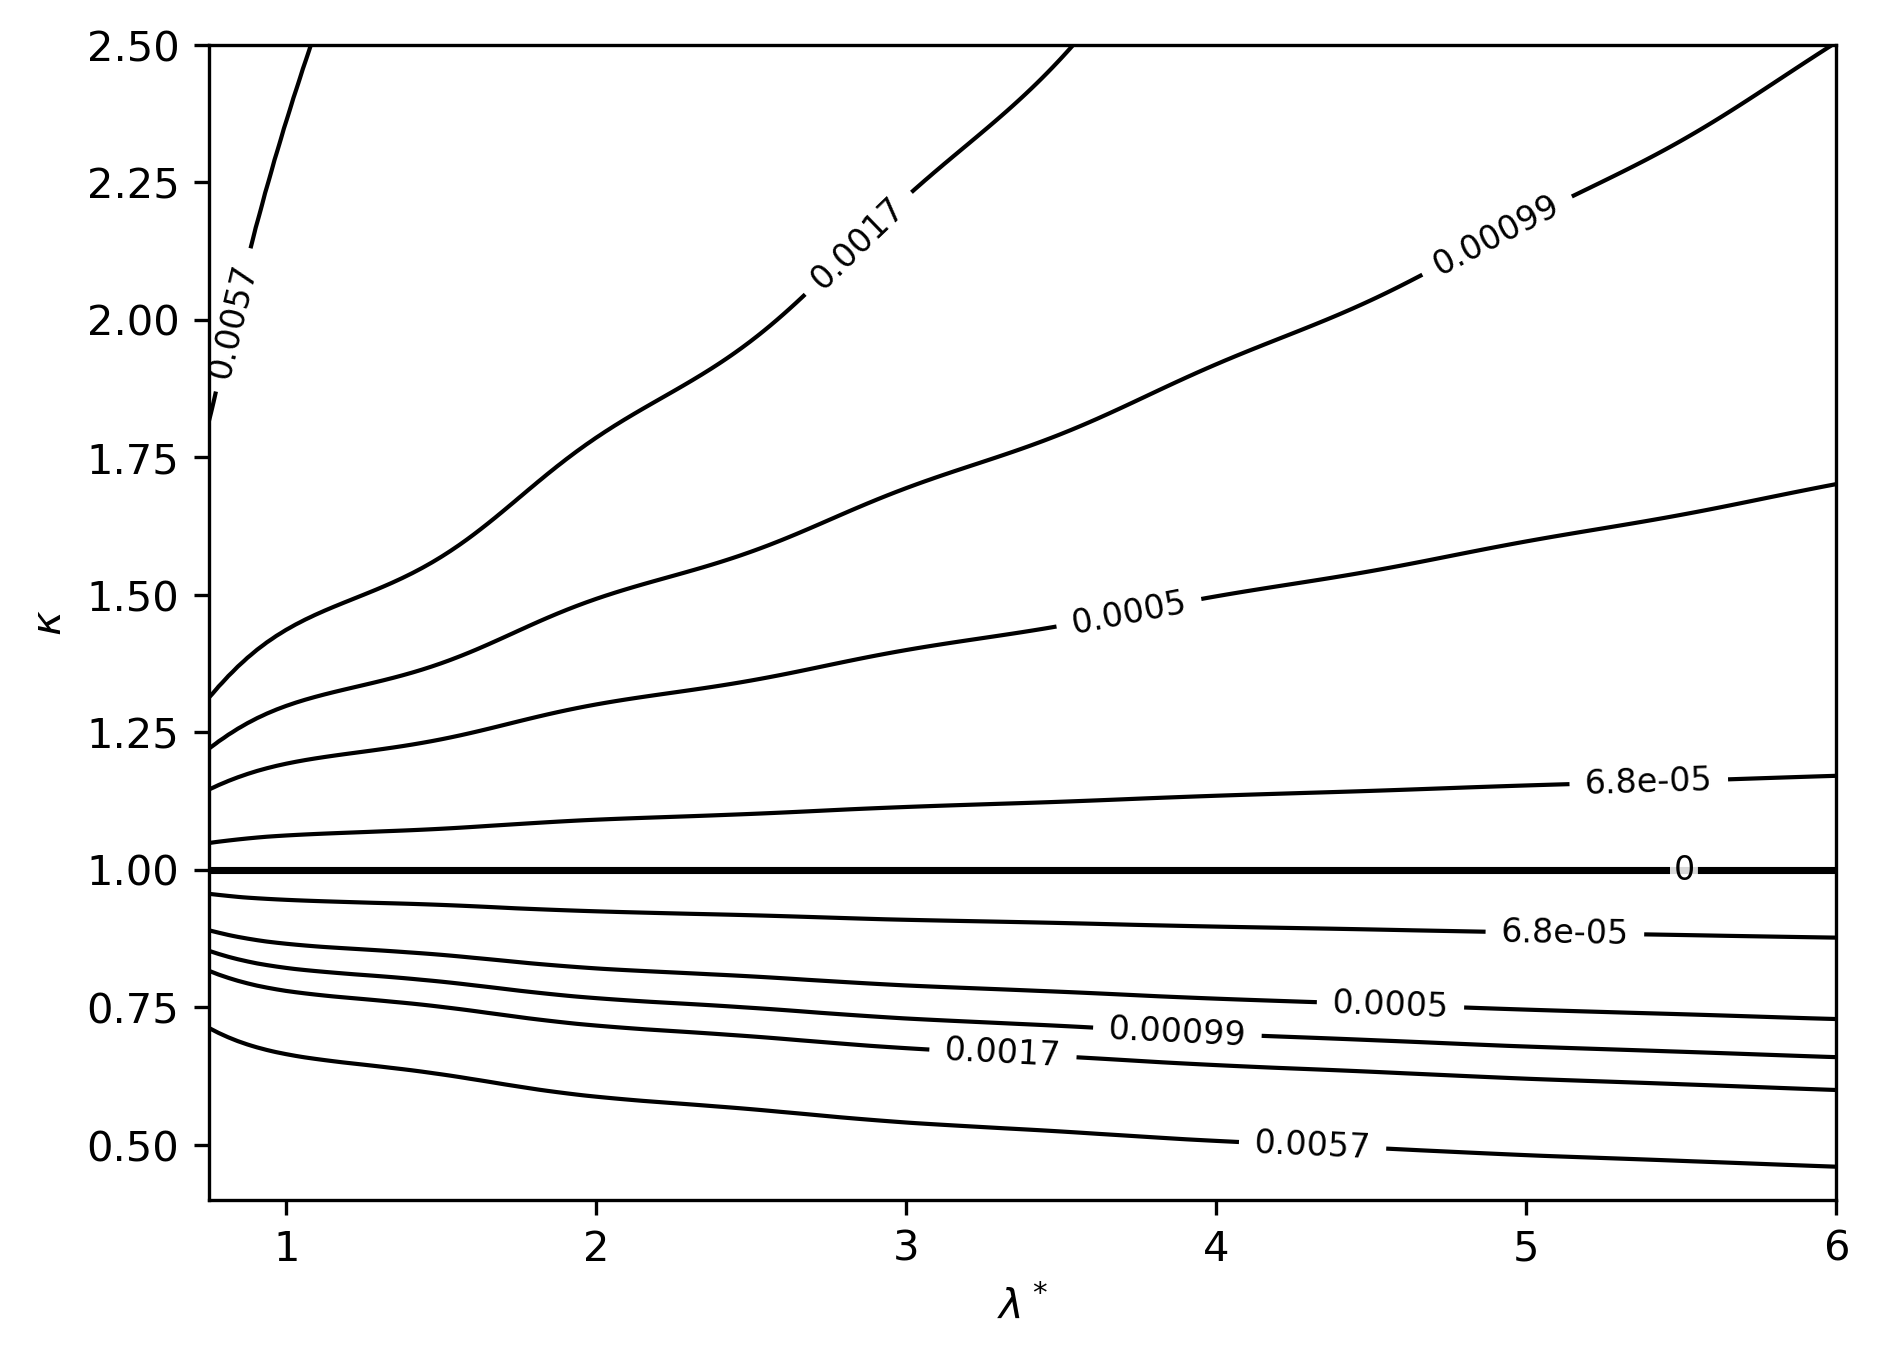
\includegraphics[width=0.82\textwidth]{images/main_J_isolines.png}
	\caption{Изолинии квадратичного функционала на основной области}
	\label{fig:chap2_main_j_isolines}
\end{figure}

На рис.~\ref{fig:chap2_main_j_isolines} показана структура квадратичного функционала в координатах $\lambda^\star$ и $\kappa$. Рационально-тригонометрическая структура конечной формулы позволяет воспроизводить как общий спад функционала при росте витковой дальности, так и остаточные колебания вдоль кривой локальных оптимумов.

Полученные конечные формулы допускают как прямое, так и обратное использование. В прямой постановке по заданной дате старта вычисляется начальная синодическая фаза, затем определяются допустимые значения $\widehat{\lambda}^{\star}_{k}$, после чего находятся продолжительность перелёта и значение функционала. В обратной постановке заданные ограничения на продолжительность перелёта, функционал или витковую дальность могут использоваться для восстановления допустимых значений начальной синодической фазы и соответствующих дат старта. В настоящей главе это свойство рассматривается как следствие структуры кривой локальных оптимумов; его алгоритмическое применение будет использовано далее при построении начального приближения.

\section{Конечные формулы для параметров оптимального управления}

Помимо продолжительности перелёта, непрерывной фазы и квадратичного функционала, для построения начального приближения необходимо аппроксимировать параметры оптимального управления. В соответствии с обозначениями, введёнными в главе~1, такими параметрами являются начальные значения сопряжённых переменных. В плоской задаче они образуют вектор
\begin{equation}
	\mathbf z_0=
	\left(
	p_{rx}(t_0),
	p_{ry}(t_0),
	p_{vx}(t_0),
	p_{vy}(t_0)
	\right).
\end{equation}
Далее рассматриваются конечные формулы для этих величин на кривой локальных оптимумов.

Решение двухточечной краевой задачи чувствительно к выбору начальных значений сопряжённых переменных, поэтому их аппроксимация имеет не только описательный, но и прикладной смысл. Зная параметры оптимального управления, можно построить начальное приближение для последующей численной оптимизации в более сложной постановке.

\begin{figure}[htbp]
	\centering
	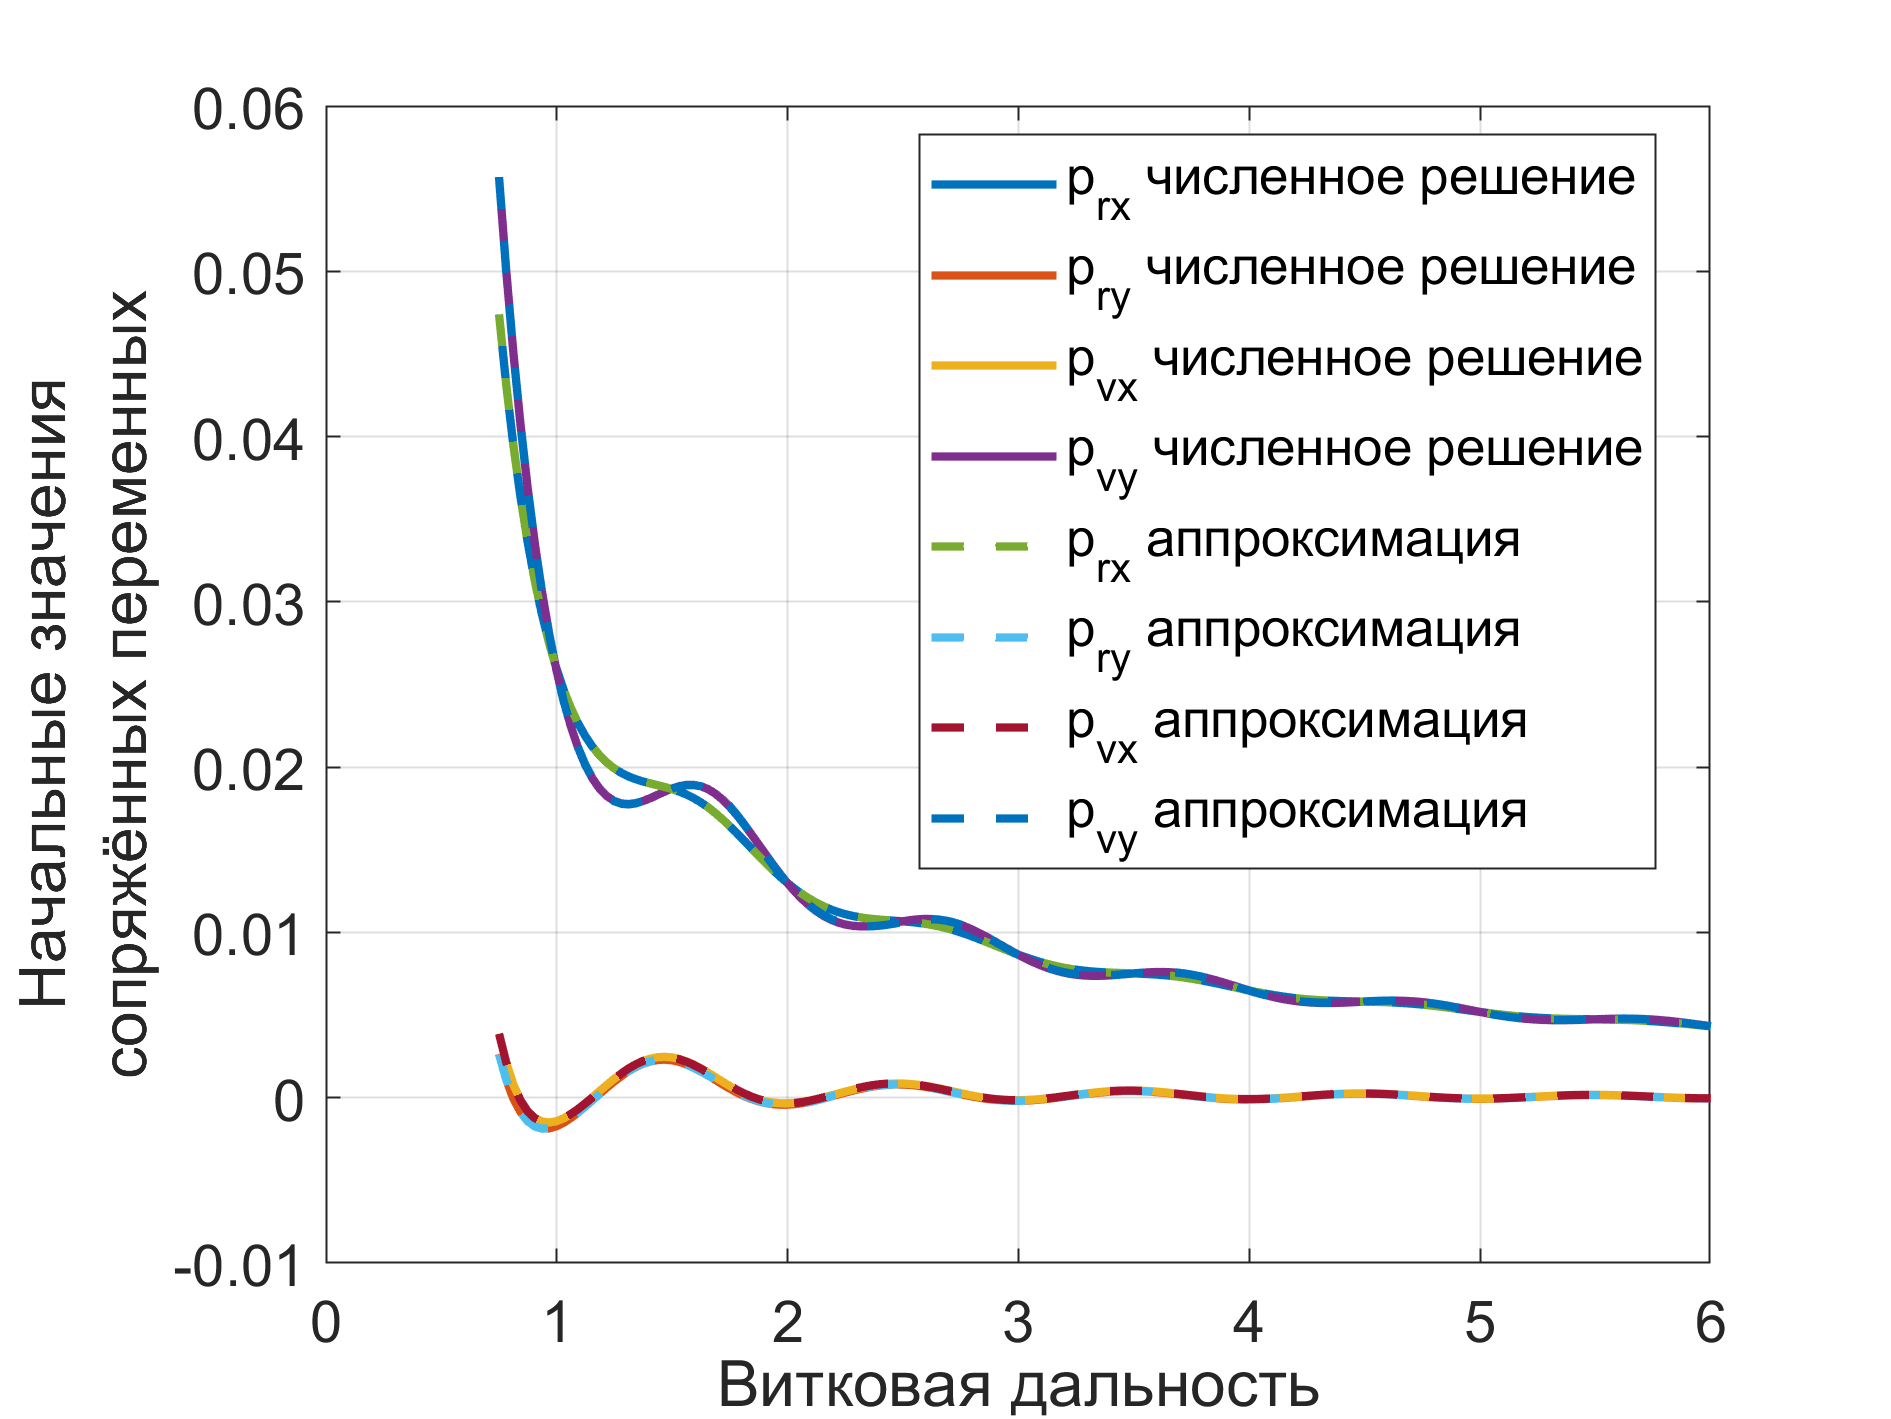
\includegraphics[width=0.82\textwidth]{images/POpt.png}
	\caption{Поведение параметров оптимального управления вдоль кривой локальных оптимумов}
	\label{fig:chap2_popt}
\end{figure}

На рис.~\ref{fig:chap2_popt} показано поведение начальных значений сопряжённых переменных вдоль кривой локальных оптимумов. Видно, что зависимости имеют выраженную попарную структуру. Первая пара образуется компонентами $p_{rx}(t_0)$ и $p_{vy}(t_0)$, вторая --- компонентами $p_{ry}(t_0)$ и $p_{vx}(t_0)$. Внутри каждой пары компоненты имеют близкий характер изменения и допускают запись в симметричном виде.

Для компактной записи конечных формул введём обозначение
\begin{equation}
	\widehat{\mathbf z}_0=
	\left(
	\widehat{p}_{rx},
	\widehat{p}_{ry},
	\widehat{p}_{vx},
	\widehat{p}_{vy}
	\right).
\end{equation}
В формулах ниже коэффициенты $C$ и параметры $D$ записываются как константы. При фиксированном значении $\kappa$ это именно числовые коэффициенты; в общем случае они являются функциями отношения радиусов. Громоздкие зависимости этих коэффициентов от $\kappa$ вынесены в приложение~Б.

Для первой пары компонент используется дробно-тригонометрическая структура
\begin{equation}
	\widehat{p}_{rx}\left(\lambda^\star\right)=
	\frac{
		C^{rx}_0
	}{
		C^{rx}_1\lambda^\star
		+
		C^{rx}_2
		+
		\sin\left(
		2\pi\lambda^\star
		+
		C^{rx}_3
		+
		D^{rx}_1\left(\lambda^\star\right)
		\right)
		+
		D^{rx}_0\left(\lambda^\star\right)
	},
\end{equation}
\begin{equation}
	\widehat{p}_{vy}\left(\lambda^\star\right)=
	\frac{
		C^{vy}_0
	}{
		C^{vy}_1\lambda^\star
		+
		C^{vy}_2
		+
		\sin\left(
		2\pi\lambda^\star
		+
		C^{vy}_3
		+
		D^{vy}_1\left(\lambda^\star\right)
		\right)
		+
		D^{vy}_0\left(\lambda^\star\right)
	}.
\end{equation}
Для второй пары компонент используется другая, но также попарно симметричная структура:
\begin{equation}
	\widehat{p}_{ry}\left(\lambda^\star\right)=
	\frac{
		C^{ry}_0
		+
		C^{ry}_1
		\cos\left(
		2\pi\lambda^\star
		+
		D^{ry}\left(\lambda^\star\right)
		\right)
	}{
		\left(\lambda^\star\right)^2
		+
		C^{ry}_2\lambda^\star
		+
		C^{ry}_3
	},
\end{equation}
\begin{equation}
	\widehat{p}_{vx}\left(\lambda^\star\right)=
	\frac{
		C^{vx}_0
		+
		C^{vx}_1
		\cos\left(
		2\pi\lambda^\star
		+
		D^{vx}\left(\lambda^\star\right)
		\right)
	}{
		\left(\lambda^\star\right)^2
		+
		C^{vx}_2\lambda^\star
		+
		C^{vx}_3
	}.
\end{equation}

Коэффициенты $C$ задают основную часть зависимости и определяются по результатам символьной регрессии. Однако одних $C$-коэффициентов оказывается недостаточно для равномерного описания всей области значений $\lambda^\star$. В области малой витковой дальности существенную роль играют дополнительные поправочные функции $D$.

Для компонент $p_{rx}(t_0)$ и $p_{vy}(t_0)$ используются по две поправочные функции:
\begin{equation}
	D^{rx}_0\left(\lambda^\star\right)=
	\left(
	D^{rx}_{0,0}
	+
	D^{rx}_{0,1}\lambda^\star
	+
	D^{rx}_{0,2}\left(\lambda^\star\right)^2
	\right)
	\exp\left(
	D^{rx}_{0,3}\lambda^\star
	\right),
\end{equation}
\begin{equation}
	D^{rx}_1\left(\lambda^\star\right)=
	\frac{
		D^{rx}_{1,0}
	}{
		\left(\lambda^\star\right)^2
		+
		D^{rx}_{1,1}\lambda^\star
		+
		D^{rx}_{1,2}
	},
\end{equation}
\begin{equation}
	D^{vy}_0\left(\lambda^\star\right)=
	\left(
	D^{vy}_{0,0}\left(\lambda^\star\right)^2
	+
	D^{vy}_{0,1}\lambda^\star
	+
	D^{vy}_{0,2}
	\right)
	\exp\left(
	D^{vy}_{0,3}\lambda^\star
	\right),
\end{equation}
\begin{equation}
	D^{vy}_1\left(\lambda^\star\right)=
	\frac{
		D^{vy}_{1,0}
	}{
		\left(\lambda^\star\right)^2
		+
		D^{vy}_{1,1}\lambda^\star
		+
		D^{vy}_{1,2}
	}.
\end{equation}
Для компонент $p_{ry}(t_0)$ и $p_{vx}(t_0)$ поправочные функции входят в фазу косинуса:
\begin{equation}
	D^{ry}\left(\lambda^\star\right)=
	\left(
	D^{ry}_{0}\left(\lambda^\star\right)^2
	+
	D^{ry}_{1}\lambda^\star
	+
	D^{ry}_{2}
	\right)
	\exp\left(
	D^{ry}_{3}\lambda^\star
	+
	D^{ry}_{4}\left(\lambda^\star\right)^2
	\right),
\end{equation}
\begin{equation}
	D^{vx}\left(\lambda^\star\right)=
	\left(
	D^{vx}_{0}\left(\lambda^\star\right)^2
	+
	D^{vx}_{1}\lambda^\star
	+
	D^{vx}_{2}
	\right)
	\exp\left(
	D^{vx}_{3}\lambda^\star
	+
	D^{vx}_{4}\left(\lambda^\star\right)^2
	\right).
\end{equation}

Функции $D$ быстро убывают при росте витковой дальности и становятся пренебрежимо малыми в многовитковой области. Поэтому они описывают прежде всего переходную область малой витковой дальности. Их введение позволяет сшить мало- и многовитковые решения одной конечной формулой, а также повысить точность определения $C$-коэффициентов за счёт раздельного описания основной зависимости и локальной поправки.

При построении этих выражений дополнительно проверялось отсутствие нулей в знаменателях на рассматриваемой области определения. Это важно, поскольку конечные формулы должны использоваться не только для описания уже построенных точек, но и для последующего вычисления начальных приближений.

Итоговый вид блока конечных формул является компромиссным. Он был получен не прямым переносом одной сырой аппроксимации PySR, а согласованием и смешением аппроксимаций, построенных для двух характерных значений отношения радиусов, $\kappa=0.72$ и $\kappa=1.52$. Такой подход позволил сохранить компактность записи и одновременно получить устойчивую структуру, пригодную для дальнейшего расширения по параметру $\kappa$.

\begin{figure}[htbp]
	\centering
	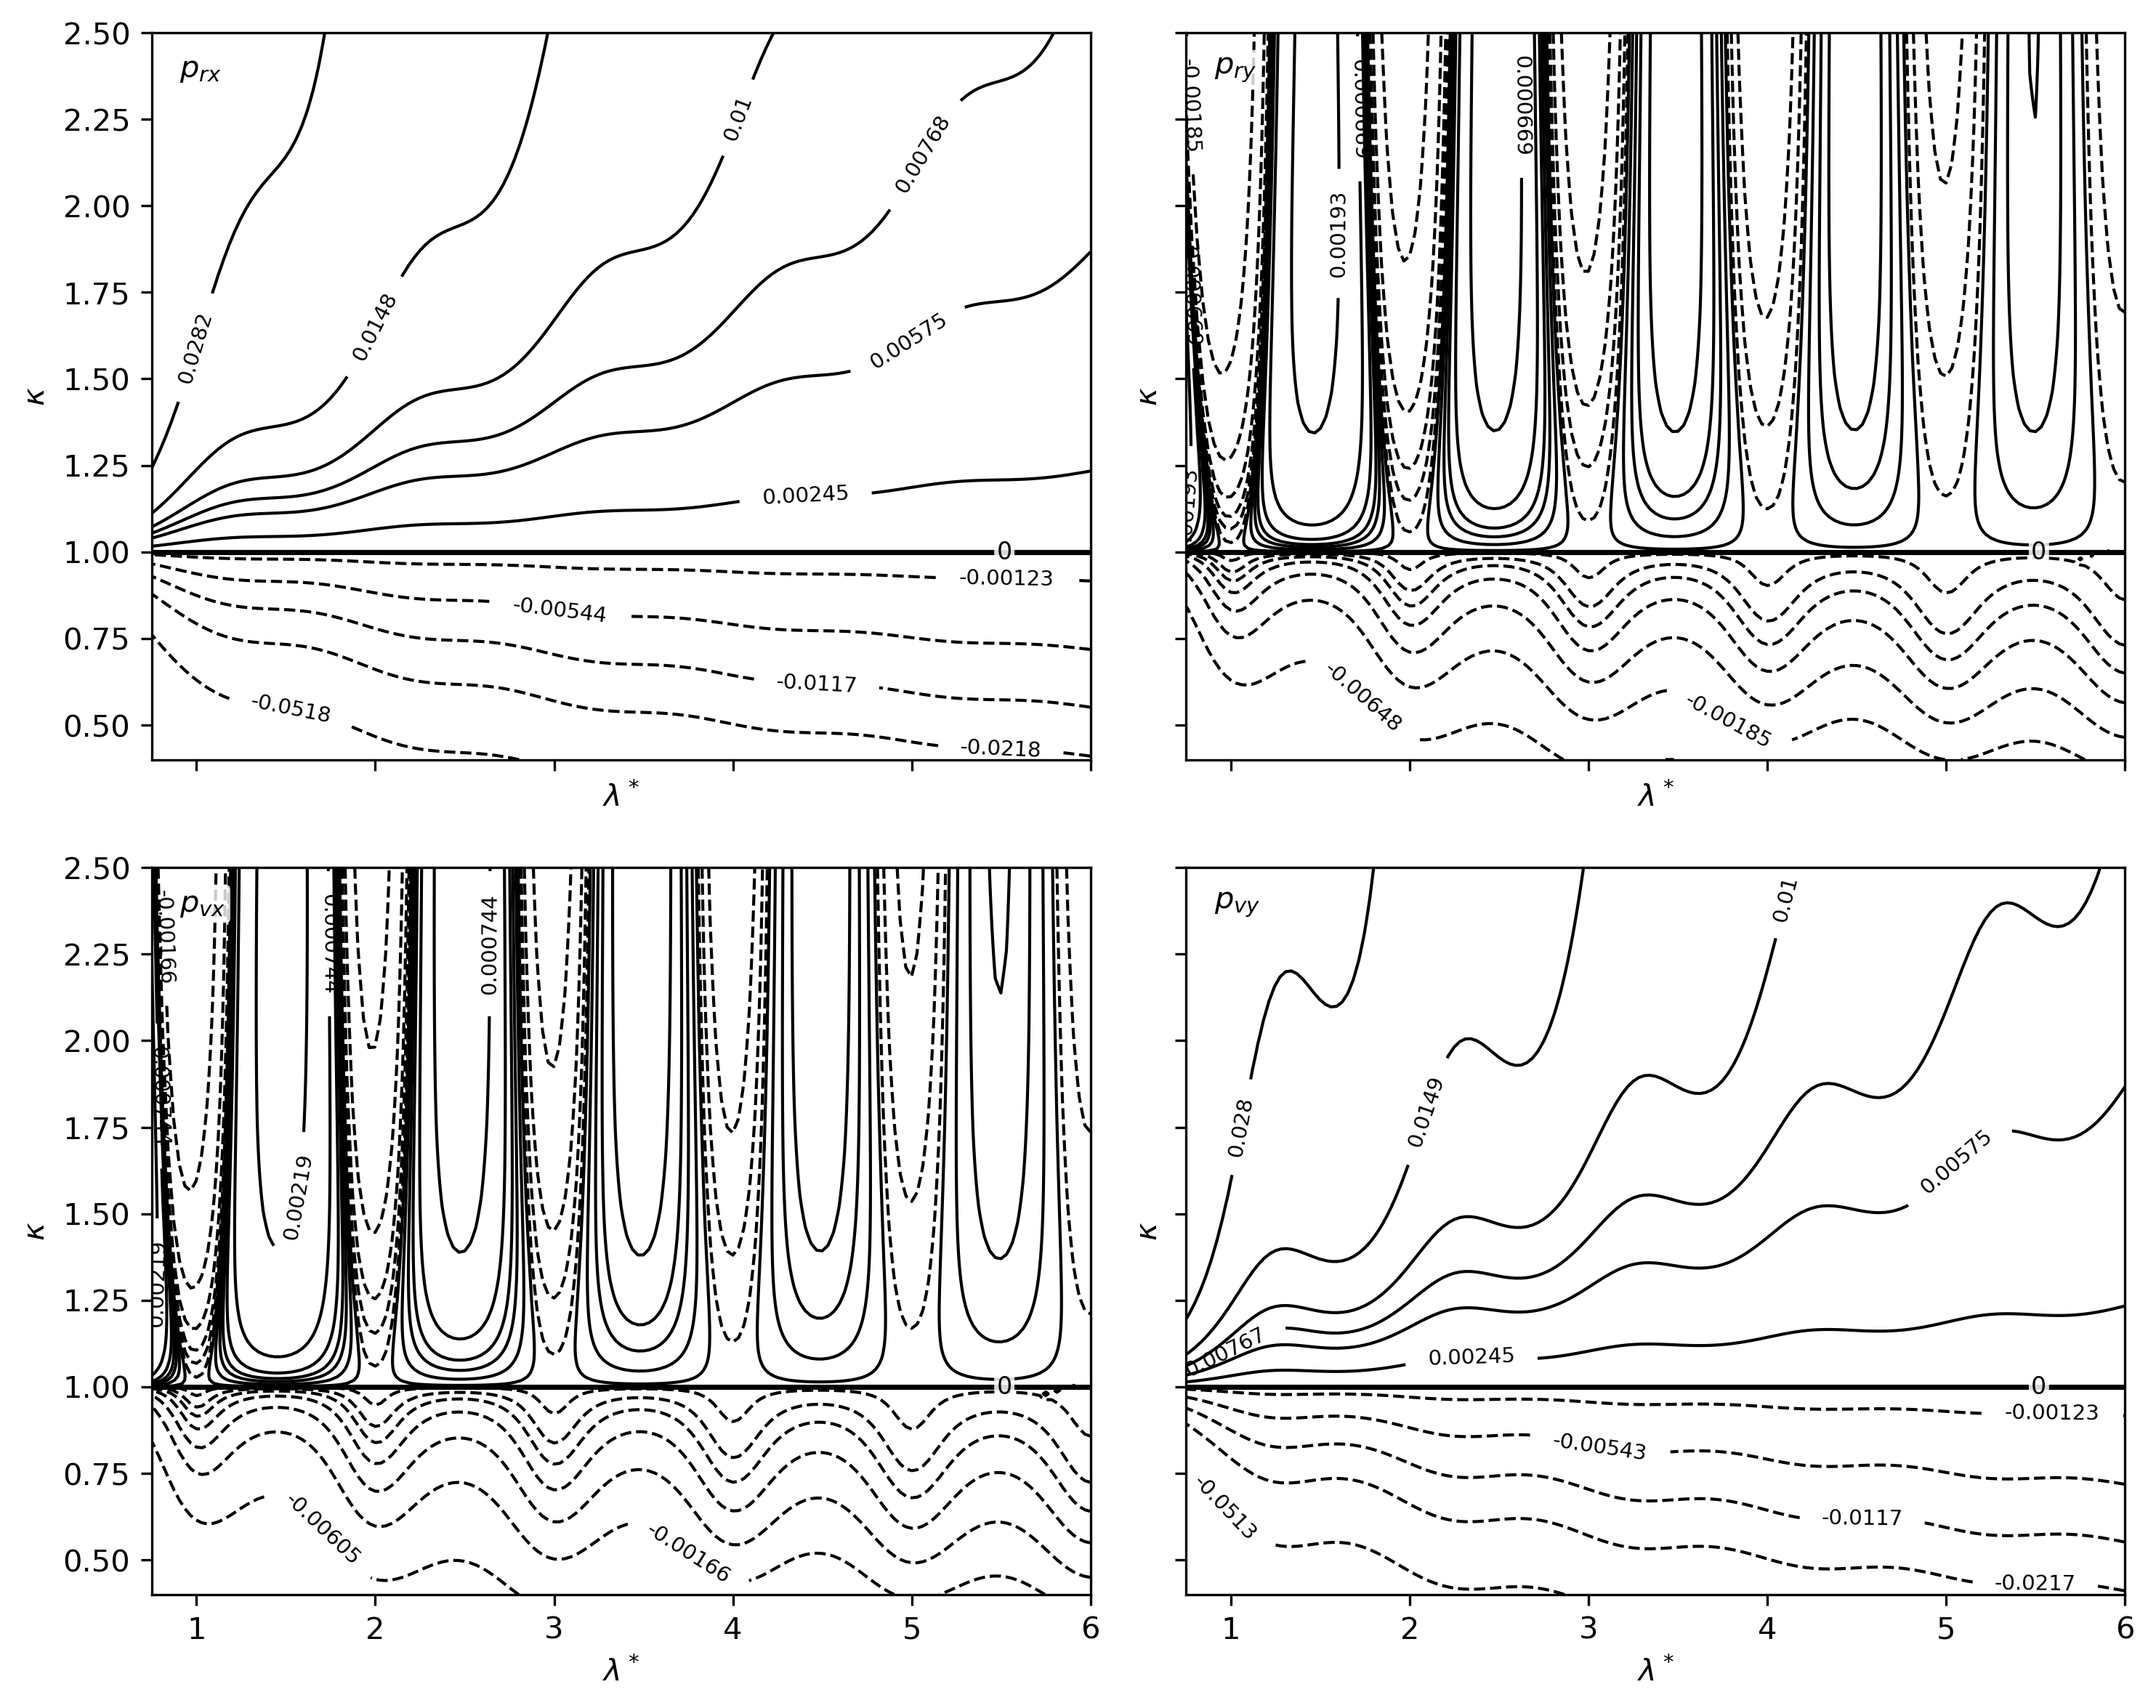
\includegraphics[width=0.82\textwidth]{images/main_p_isolines.png}
	\caption{Изолинии параметров оптимального управления на основной области}
	\label{fig:chap2_main_p_isolines}
\end{figure}

На рис.~\ref{fig:chap2_main_p_isolines} показаны структуры компонент параметров оптимального управления при изменении $\lambda^\star$ и $\kappa$. Этот рисунок подтверждает, что попарная структура сохраняется не только при фиксированном отношении радиусов, но и на диапазоне значений $\kappa$. Громоздкие выражения для двумерных коэффициентов вынесены в приложение~Б.

Причина наблюдаемой разделяемости на основную часть с $C$-коэффициентами и быстро затухающие $D$-функции в настоящей работе не выводится аналитически. В дальнейшем она используется как устойчиво наблюдаемая численная структура, позволяющая получить компактные конечные формулы для параметров оптимального управления.

Таким образом, конечные формулы для начальных значений сопряжённых переменных дополняют зависимости для продолжительности перелёта, непрерывной фазы и квадратичного функционала. Вместе они позволяют восстановить полный набор характеристик решения на кривой локальных оптимумов. В следующем разделе будет рассмотрен дополнительный набор конечных формул для области малой витковой дальности.

\section{Дополнительные конечные формулы для продолжительности перелёта, непрерывной фазы и квадратичного функционала в области малой витковой дальности}

Основные конечные формулы, рассмотренные выше, строились для рабочей области кривой локальных оптимумов. Однако при дальнейшем использовании этих зависимостей в задаче построения начального приближения возможно прохождение через область малой витковой дальности. Поэтому для устойчивости вычислительной процедуры дополнительно были построены конечные формулы в области
\begin{equation}
	\lambda^\star < 0.75.
\end{equation}
Эта область не является основной для дальнейшего баллистического проектирования, однако она важна как переходная зона, в которой сохраняется возможность непрерывного продолжения решения.

В маловитковой области зависимости имеют менее регулярный вид, а качество аппроксимаций оказывается ниже, чем в основной области. Тем не менее общая логика построения сохраняется: конечные формулы задаются как функции локально оптимальной витковой дальности $\lambda^\star$ и отношения радиусов $\kappa$. В данном разделе рассматриваются формулы для продолжительности перелёта, нормированной непрерывной фазы и квадратичного функционала.

Для продолжительности перелёта используется конечная формула
\begin{equation}
	\begin{split}
		\widehat{T}_{\mathrm{short}}\left(\lambda^\star,\kappa\right)
		=
		\frac{
			\left(C^T_1\kappa+C^T_0\right)
			\left(\lambda^\star\right)^{-\kappa}
		}{
			\lambda^\star+C^T_4
		}
		\Big[
		&\left(\lambda^\star\right)^{\kappa+1}
		\left(\lambda^\star+C^T_4\right)
		\\
		&-
		\kappa
		\left(
		\left(C^T_2\right)^\kappa
		\ln\left(\kappa+\lambda^\star\right)
		-
		C^T_3
		\right)
		\Big].
	\end{split}
\end{equation}
Эта запись является упрощённой формой выражения, полученного методом символьной регрессии. Коэффициенты $C^T_N$ приведены в табл.~\ref{tab:chap2_short_scalar_coefficients}.

\begin{figure}[htbp]
	\centering
	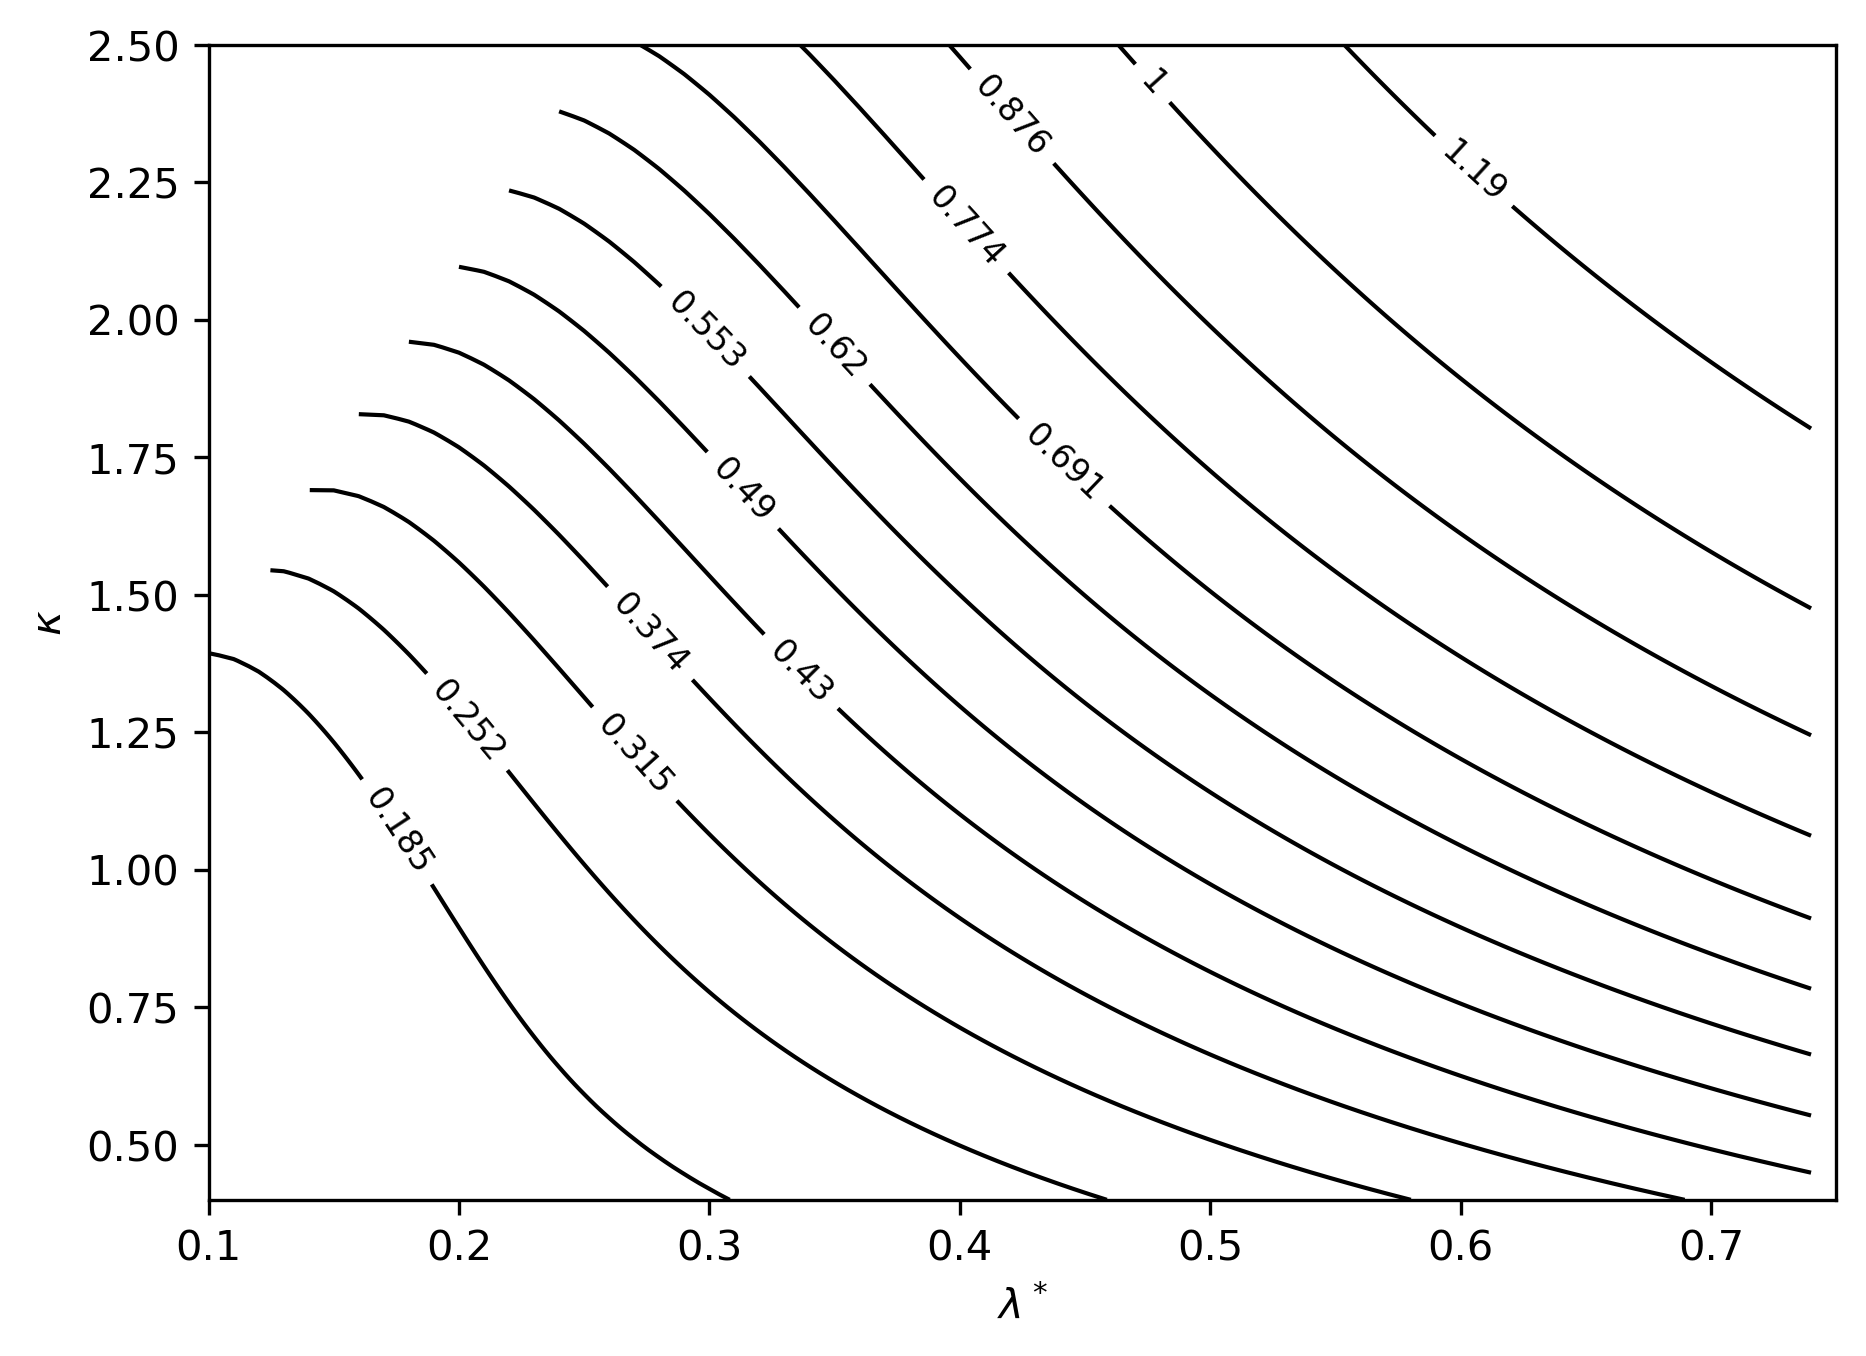
\includegraphics[width=0.82\textwidth]{images/short_T_isolines.png}
	\caption{Изолинии продолжительности перелёта в области малой витковой дальности}
	\label{fig:chap2_short_t_isolines}
\end{figure}

На рис.~\ref{fig:chap2_short_t_isolines} показана структура продолжительности перелёта в области малой витковой дальности. По сравнению с основной областью зависимость имеет более выраженную кривизну, что и приводит к необходимости отдельной конечной формулы.

Для нормированной непрерывной фазы используется выражение
\begin{equation}
	\begin{split}
		\widehat{\Psi}_{\mathrm{short}}\left(\lambda^\star,\kappa\right)
		=
		C^\Psi_0
		\frac{\kappa-C^\Psi_1}{\kappa}
		\Bigg[
		\lambda^\star
		+
		C^\Psi_2
		\frac{
			\left(\kappa^{\lambda^\star}-\kappa\right)
			\cos\left(\lambda^\star/C^\Psi_3\right)
		}{
			\kappa\left(\lambda^\star\right)^2+C^\Psi_4
		}
		\Bigg].
	\end{split}
\end{equation}
Эта формула аппроксимирует именно непрерывную развёртку фазы, а не разрывную начальную синодическую фазу.

\begin{figure}[htbp]
	\centering
	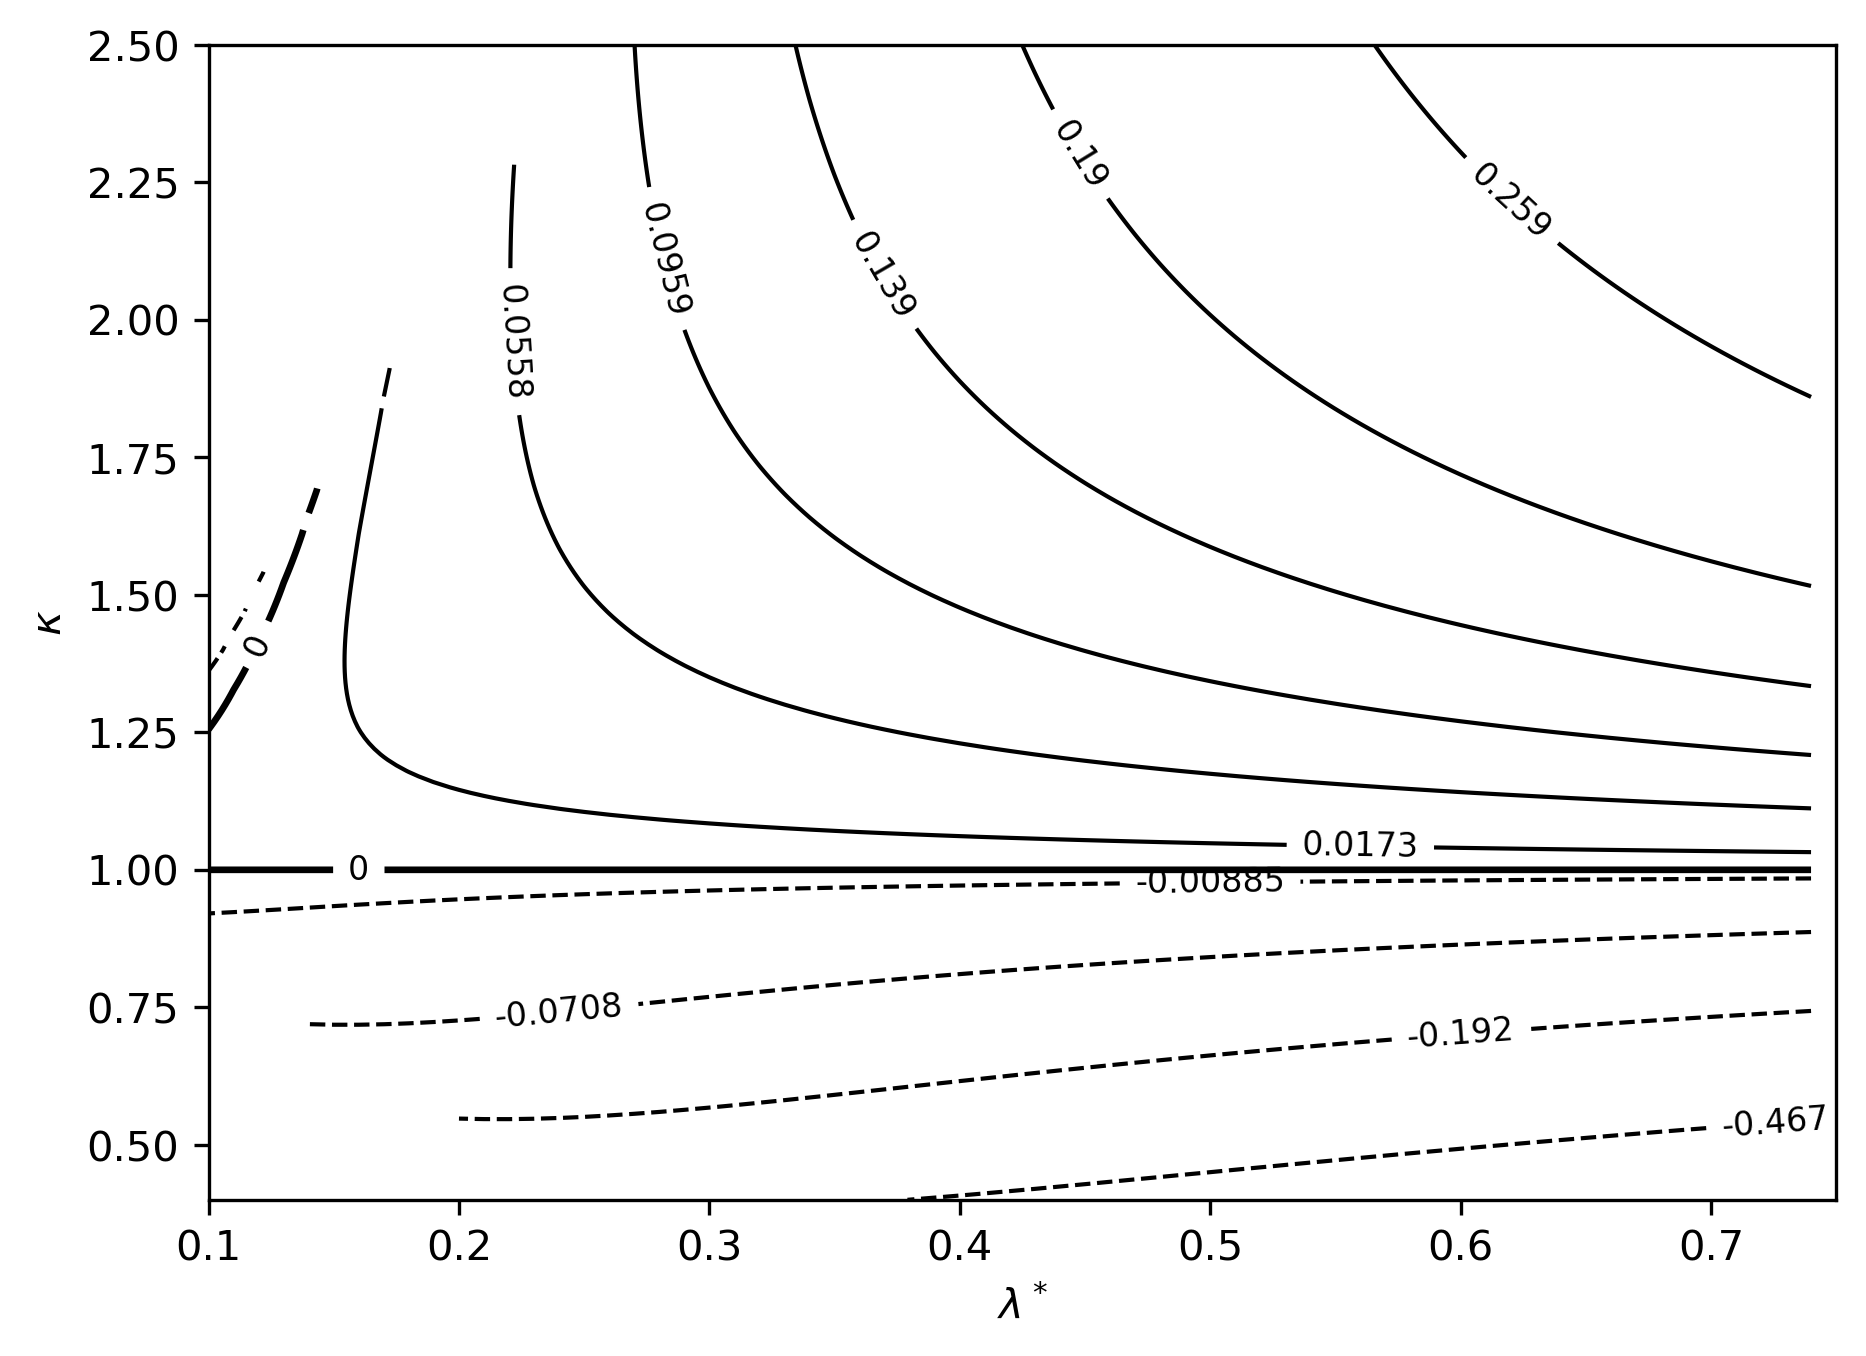
\includegraphics[width=0.82\textwidth]{images/short_phase_isolines.png}
	\caption{Изолинии нормированной непрерывной фазы в области малой витковой дальности}
	\label{fig:chap2_short_phase_isolines}
\end{figure}

На рис.~\ref{fig:chap2_short_phase_isolines} показаны изолинии нормированной непрерывной фазы. Видно, что в маловитковой области сохраняется возможность гладкого описания фазовой зависимости, однако её форма отличается от основной области и требует отдельной аппроксимации.

Для квадратичного функционала используется конечная формула
\begin{equation}
	\begin{split}
		\widehat{J}_{\mathrm{short}}\left(\lambda^\star,\kappa\right)
		=
		\left[
		\kappa
		\left(
		C^J_0\lambda^\star-C^J_1
		\right)
		\right]^{-C^J_2}
		\ln\kappa
		\arctan
		\left(
		C^J_3
		\frac{
			\ln\kappa\cos\lambda^\star
		}{
			\left(\lambda^\star\right)^2
		}
		\right).
	\end{split}
\end{equation}
В отличие от основной области, здесь формула носит более выраженный эмпирический характер. Она используется для сохранения работоспособности приближённого описания в переходной области, а не как основной инструмент анализа энергетической структуры решений.

\begin{figure}[htbp]
	\centering
	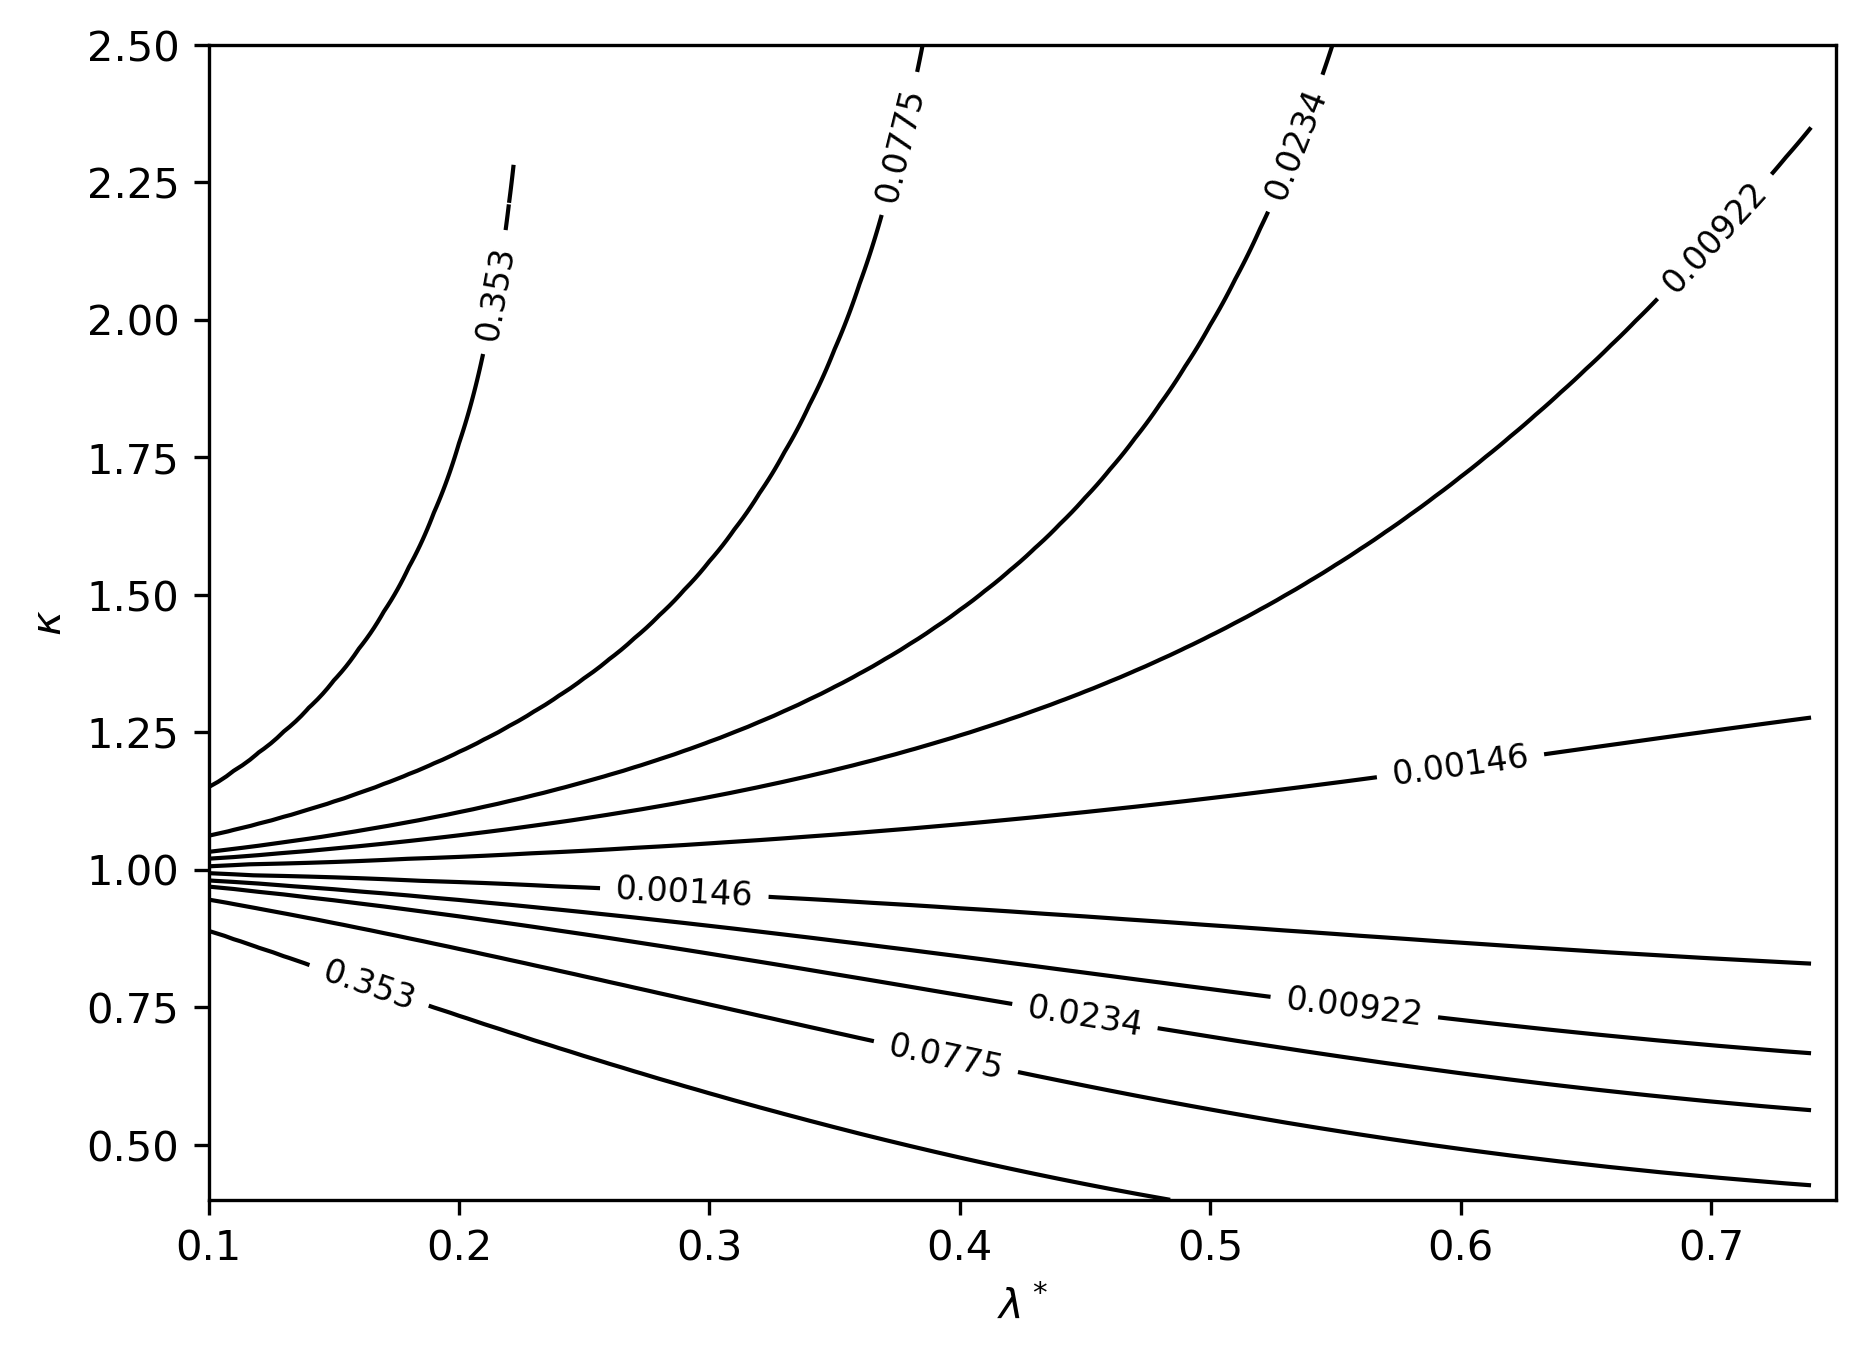
\includegraphics[width=0.82\textwidth]{images/short_J_isolines.png}
	\caption{Изолинии квадратичного функционала в области малой витковой дальности}
	\label{fig:chap2_short_j_isolines}
\end{figure}

На рис.~\ref{fig:chap2_short_j_isolines} показана структура квадратичного функционала в области малой витковой дальности. Эта зависимость менее регулярна, чем в основной области, что согласуется с более низким качеством аппроксимаций, которое будет количественно оценено в разделе~2.9.

\begin{table}[htbp]
	\centering
	\caption{Коэффициенты конечных формул для скалярных характеристик в области малой витковой дальности}
	\label{tab:chap2_short_scalar_coefficients}
	\begin{tabular}{|c|c|c|c|}
		\hline
		$N$ & $C^T$ & $C^\Psi$ & $C^J$ \\
		\hline
		0 & $2.4717593\mathrm{E}{-1}$ & $7.580183\mathrm{E}{-1}$ & $3.3561635$ \\
		1 & $7.521363\mathrm{E}{-1}$ & $9.992080\mathrm{E}{-1}$ & $1.733732\mathrm{E}{-2}$ \\
		2 & $1.4925372\mathrm{E}{-3}$ & $1.1058738\mathrm{E}{-2}$ & $1.2552159$ \\
		3 & $3.217671\mathrm{E}{-4}$ & $3.9470634\mathrm{E}{-1}$ & $6.52341424114181\mathrm{E}{-2}$ \\
		4 & $9.116870\mathrm{E}{-2}$ & $9.082422\mathrm{E}{-3}$ & --- \\
		\hline
	\end{tabular}
\end{table}

Таким образом, для области малой витковой дальности построен отдельный набор конечных формул для скалярных характеристик. Эти зависимости дополняют основные формулы главы и обеспечивают непрерывность приближённого описания при проходе через маловитковую область. Конечные формулы для параметров оптимального управления в этой же области рассматриваются в следующем разделе.


\section{Дополнительные конечные формулы для параметров оптимального управления в области малой витковой дальности}

В области малой витковой дальности дополнительно аппроксимируются параметры оптимального управления. Как и в основной области, речь идёт о начальных значениях сопряжённых переменных
\begin{equation}
	\mathbf z_{0,\mathrm{short}}=
	\left(
	p_{rx,\mathrm{short}},
	p_{ry,\mathrm{short}},
	p_{vx,\mathrm{short}},
	p_{vy,\mathrm{short}}
	\right).
\end{equation}
Эти формулы используются как техническое расширение основного набора конечных формул и обеспечивают возможность прохода вычислительной процедуры через область $\lambda^\star<0.75$.

В отличие от основной области, здесь не удаётся сохранить столь же регулярную попарную структуру. Зависимости начальных значений сопряжённых переменных имеют более выраженный эмпирический характер, поэтому для каждой компоненты используется отдельная конечная формула. При этом все формулы задаются как функции локально оптимальной витковой дальности $\lambda^\star$ и отношения радиусов $\kappa$.

Для первой компоненты используется выражение
\begin{equation}
	\begin{aligned}
		\widehat{p}_{rx,\mathrm{short}}
		&=
		\frac{
			\sin\!\left(
			C^{rx}_0
			\left(C^{rx}_1\right)^{\kappa}
			\left(\lambda^\star\right)^{C^{rx}_2}
			\ln\kappa
			\right)
		}{
			\left(C^{rx}_3\lambda^\star-C^{rx}_4\right)
			\arctan\!\left(
			\kappa\lambda^\star
			+
			C^{rx}_5\kappa
			+
			C^{rx}_5\lambda^\star
			\right)
		}.
	\end{aligned}
\end{equation}

Для второй компоненты конечная формула имеет вид
\begin{equation}
	\begin{aligned}
		\widehat{p}_{ry,\mathrm{short}}
		&=
		C^{ry}_0
		\Bigg(
		\left(\lambda^\star\right)^{C^{ry}_1}
		\left[
		\left(C^{ry}_2\right)^\kappa
		-
		C^{ry}_3
		\right]
		+
		\frac{\lambda^\star}{
			\ln\!\left(
			\exp\!\left(\arctan\kappa\right)
			\cos\lambda^\star
			\right)
		}
		+
		C^{ry}_4
		\Bigg)
		\\
		&\quad {}\times
		\arctan\!\left(
		\frac{
			C^{ry}_5\ln\kappa
		}{
			\kappa
			\left[
			\left(C^{ry}_6\right)^{\lambda^\star}
			-
			\cos\lambda^\star
			\right]
		}
		\right).
	\end{aligned}
\end{equation}

Для третьей компоненты используется выражение
\begin{equation}
	\begin{aligned}
		\widehat{p}_{vx,\mathrm{short}}
		&=
		\Bigg(
		\sin\!\left(
		\left[
		\frac{
			C^{vx}_0\kappa^{C^{vx}_1}
		}{
			\lambda^\star
		}
		+
		C^{vx}_2
		\right]
		\ln\kappa
		+
		C^{vx}_3
		\right)
		-
		C^{vx}_4
		\Bigg)
		\\
		&\quad {}\times
		\Bigg(
		\arctan\!\left(
		\arctan\!\left(
		\sin\!\left(
		C^{vx}_5\kappa\lambda^\star
		\right)
		\right)
		\right)
		-
		C^{vx}_6
		-
		\frac{C^{vx}_7}{\lambda^\star}
		\Bigg).
	\end{aligned}
\end{equation}

Для четвёртой компоненты конечная формула записывается следующим образом:
\begin{equation}
	\begin{aligned}
		\widehat{p}_{vy,\mathrm{short}}
		&=
		C^{vy}_0
		\frac{
			\sin\!\left(
			\left(
			C^{vy}_1
			+
			\frac{\kappa-C^{vy}_2}{\lambda^\star}
			\right)
			\left(
			C^{vy}_3\lambda^\star
			+
			\frac{C^{vy}_4}{\kappa}
			\right)
			\right)
		}{
			\lambda^\star+C^{vy}_5
		}
		-
		\frac{
			C^{vy}_6
		}{
			\kappa\left(\lambda^\star+C^{vy}_7\right)
		}.
	\end{aligned}
\end{equation}

Численные значения коэффициентов приведены в табл.~\ref{tab:chap2_short_p_coefficients}. Таблица временно помещена в основной текст; далее она может быть перенесена в приложение вместе с другими громоздкими коэффициентами конечных формул.

\begin{table}[htbp]
	\centering
	\caption{Коэффициенты конечных формул для параметров оптимального управления в области малой витковой дальности}
	\label{tab:chap2_short_p_coefficients}
	\begin{tabular}{|c|c|c|c|c|}
		\hline
		$N$ & $C^{rx}$ & $C^{ry}$ & $C^{vx}$ & $C^{vy}$ \\
		\hline
		0 & $3.672486\mathrm{E}{-1}$ & $3.7612966\mathrm{E}{-1}$ & $-6.31448245240317\mathrm{E}{-1}$ & $2.7265343\mathrm{E}{-1}$ \\
		1 & $8.698383\mathrm{E}{-1}$ & $-2.6759982$ & $-1.0166328\mathrm{E}{-1}$ & $1.3624265$ \\
		2 & $-1.3319579$ & $2.020348\mathrm{E}{-2}$ & $7.8313917\mathrm{E}{-1}$ & $9.5281893\mathrm{E}{-1}$ \\
		3 & $4.26744541286531$ & $1.5443553\mathrm{E}{-2}$ & $2.6944399\mathrm{E}{-2}$ & $-1.4588301\mathrm{E}{-1}$ \\
		4 & $1.5451069\mathrm{E}{-1}$ & $2.7214472$ & $2.9475454\mathrm{E}{-2}$ & $7.468672\mathrm{E}{-1}$ \\
		5 & $4.4000748\mathrm{E}{-1}$ & $12.236265$ & $1.37525608987464$ & $1.00266375\mathrm{E}{-1}$ \\
		6 & --- & $7431.9634$ & $5.874708\mathrm{E}{-1}$ & $2.0214483\mathrm{E}{-1}$ \\
		7 & --- & --- & $2.0697053\mathrm{E}{-1}$ & $4.505406\mathrm{E}{-2}$ \\
		\hline
	\end{tabular}
\end{table}

\begin{figure}[htbp]
	\centering
	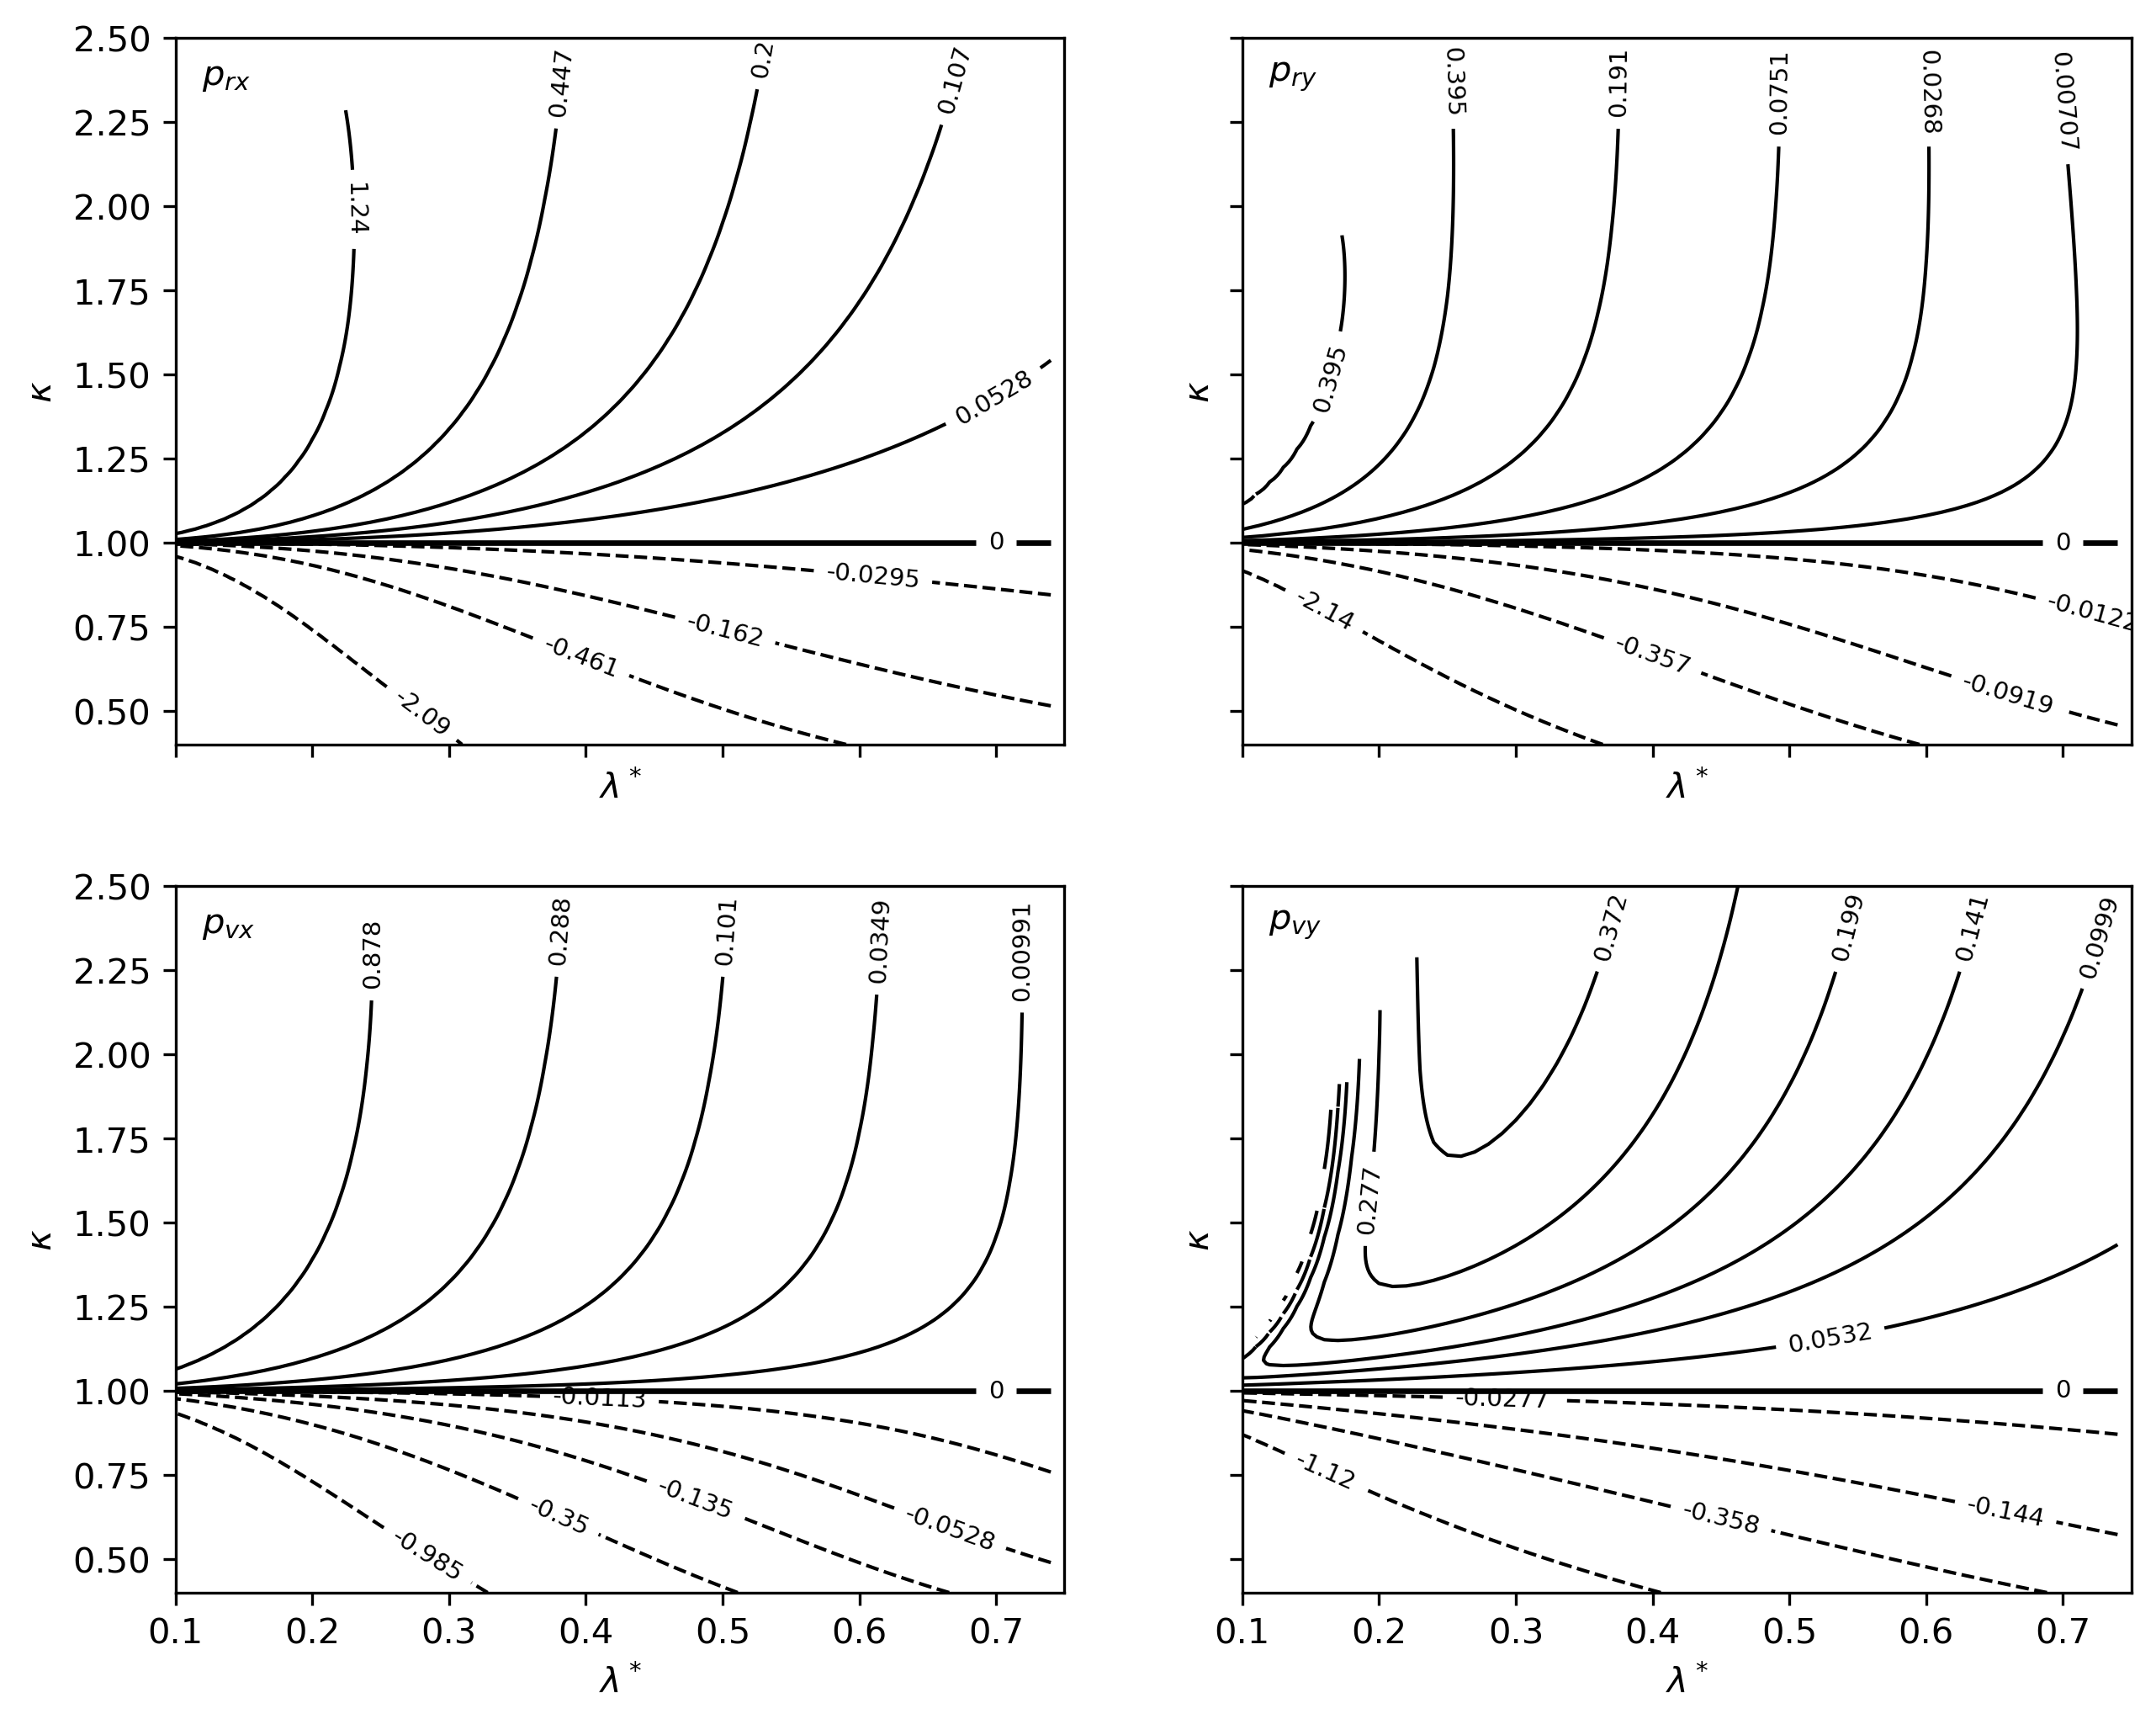
\includegraphics[width=0.82\textwidth]{images/short_p_isolines.png}
	\caption{Изолинии параметров оптимального управления в области малой витковой дальности}
	\label{fig:chap2_short_p_isolines}
\end{figure}

На рис.~\ref{fig:chap2_short_p_isolines} показана структура параметров оптимального управления в области малой витковой дальности. В отличие от основной области, здесь зависимости менее регулярны, что объясняет более сложный вид конечных формул и более низкое качество аппроксимации. Тем не менее полученный набор зависимостей позволяет восстановить начальные значения сопряжённых переменных в переходной области и тем самым дополняет основной набор конечных формул.

Таким образом, для области малой витковой дальности построены конечные формулы как для скалярных характеристик, так и для параметров оптимального управления. Вместе с формулами основной области они задают приближённое описание решений на рассматриваемом диапазоне $\lambda^\star$ и $\kappa$. В следующем разделе будет приведена количественная верификация качества построенных конечных формул.

\section{Верификация качества конечных формул}

В предыдущих разделах были построены конечные формулы для основной области и для области малой витковой дальности. Для оценки их качества использовались одни и те же метрики: характерный масштаб величины, среднеквадратическая ошибка, средняя абсолютная ошибка и максимальная абсолютная ошибка. Для скалярной величины $x$ с аппроксимацией $\widehat{x}$ ошибка в узле сетки определяется как
\begin{equation}
	e_i=\widehat{x}_i-x_i.
\end{equation}
Характерный масштаб величины задаётся среднеквадратическим значением самой величины:
\begin{equation}
	S(x)=
	\sqrt{
		\frac{1}{N}
		\sum_{i=1}^{N}x_i^2
	}.
\end{equation}
Далее используются метрики
\begin{equation}
	\mathrm{RMSE}=
	\sqrt{
		\frac{1}{N}
		\sum_{i=1}^{N}e_i^2
	},
	\qquad
	\mathrm{MAE}=
	\frac{1}{N}
	\sum_{i=1}^{N}|e_i|,
	\qquad
	\max |e|=\max_i |e_i|.
\end{equation}
Для параметров оптимального управления дополнительно рассматривается агрегированная ошибка вектора
\begin{equation}
	e_{\mathbf z,i}
	=
	\left\|
	\widehat{\mathbf z}_{0,i}
	-
	\mathbf z_{0,i}
	\right\|_2.
\end{equation}
Соответствующий масштаб задаётся выражением
\begin{equation}
	S(\mathbf z_0)=
	\sqrt{
		\frac{1}{N}
		\sum_{i=1}^{N}
		\left\|
		\mathbf z_{0,i}
		\right\|_2^2
	}.
\end{equation}

В табл.~\ref{tab:chap2_main_metrics} приведены значения метрик для основной области. Видно, что для продолжительности перелёта и непрерывной фазы ошибки малы по сравнению с характерным масштабом соответствующих величин. Для параметров оптимального управления наибольшая локальная ошибка наблюдается у компоненты $p_{rx}$, однако агрегированная среднеквадратическая ошибка вектора $\mathbf z_0$ остаётся существенно меньше его характерного масштаба.

\begin{table}[htbp]
	\centering
	\caption{Качество конечных формул в основной области}
	\label{tab:chap2_main_metrics}
	\begin{tabular}{l c c c c}
		\toprule
		Величина & Масштаб $S$ & RMSE $(\sigma)$ & MAE & $\max |e|$ \\
		\midrule
		$\widehat{T}$ &
		$4.96242$ &
		$2.31665\cdot10^{-2}$ &
		$1.46224\cdot10^{-2}$ &
		$1.44234\cdot10^{-1}$ \\
		
		$\widehat{\Psi}_{T}$ &
		$1.40529$ &
		$4.02183\cdot10^{-2}$ &
		$1.62921\cdot10^{-2}$ &
		$3.54534\cdot10^{-1}$ \\
		
		$\widehat{\Psi}$ &
		$1.40529$ &
		$1.88208\cdot10^{-2}$ &
		$1.26730\cdot10^{-2}$ &
		$1.03851\cdot10^{-1}$ \\
		
		$\widehat{J}$ &
		$5.28128\cdot10^{-3}$ &
		$1.24053\cdot10^{-4}$ &
		$3.38967\cdot10^{-5}$ &
		$2.69356\cdot10^{-3}$ \\
		
		$\widehat{p}_{rx}$ &
		$2.22306\cdot10^{-2}$ &
		$7.89681\cdot10^{-4}$ &
		$1.23858\cdot10^{-4}$ &
		$3.14925\cdot10^{-2}$ \\
		
		$\widehat{p}_{ry}$ &
		$4.89269\cdot10^{-3}$ &
		$1.42840\cdot10^{-4}$ &
		$3.66959\cdot10^{-5}$ &
		$5.31230\cdot10^{-3}$ \\
		
		$\widehat{p}_{vx}$ &
		$4.04930\cdot10^{-3}$ &
		$1.65060\cdot10^{-4}$ &
		$3.79726\cdot10^{-5}$ &
		$6.25885\cdot10^{-3}$ \\
		
		$\widehat{p}_{vy}$ &
		$2.24331\cdot10^{-2}$ &
		$2.96880\cdot10^{-4}$ &
		$7.50743\cdot10^{-5}$ &
		$8.40485\cdot10^{-3}$ \\
		
		$\widehat{\mathbf z}_{0}$ &
		$3.22146\cdot10^{-2}$ &
		$8.71425\cdot10^{-4}$ &
		$1.75271\cdot10^{-4}$ &
		$3.36127\cdot10^{-2}$ \\
		\bottomrule
	\end{tabular}
\end{table}

Локальное распределение ошибок в основной области показано на рис.~\ref{fig:chap2_main_error_heatmaps}. Наибольшие ошибки сосредоточены в отдельных областях параметров, тогда как на большей части области значения ошибок остаются малыми. Такая картина дополняет табл.~\ref{tab:chap2_main_metrics}, поскольку таблица даёт интегральные характеристики, а карты ошибок показывают их распределение по параметрам $\lambda^\star$ и $\kappa$.

\begin{figure}[htbp]
	\centering
	\begin{minipage}{0.48\textwidth}
		\centering
		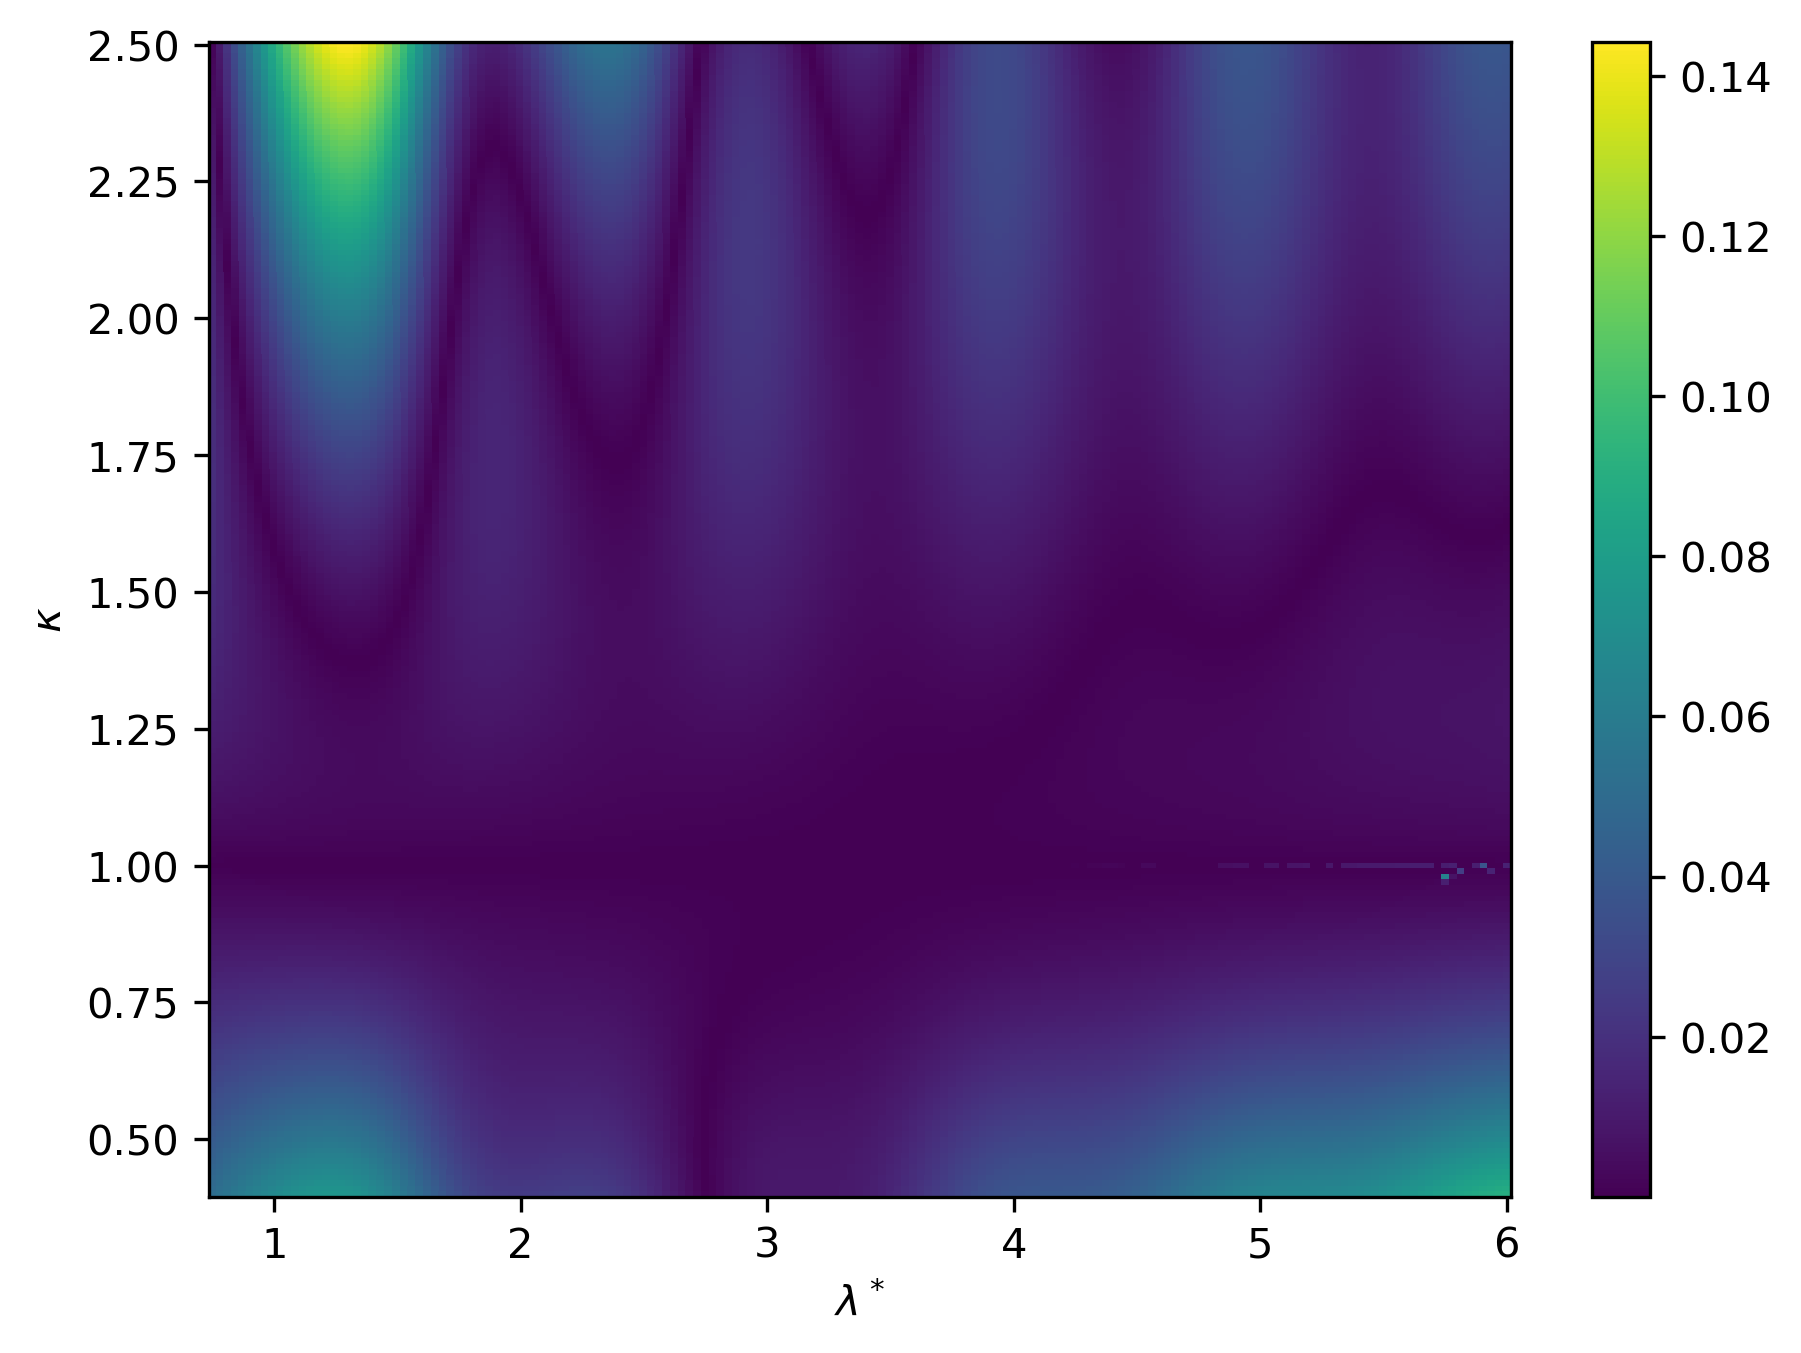
\includegraphics[width=\linewidth]{images/main_T_error_heatmap.png}
		\par\smallskip
		$\widehat{T}$
	\end{minipage}
	\hfill
	\begin{minipage}{0.48\textwidth}
		\centering
		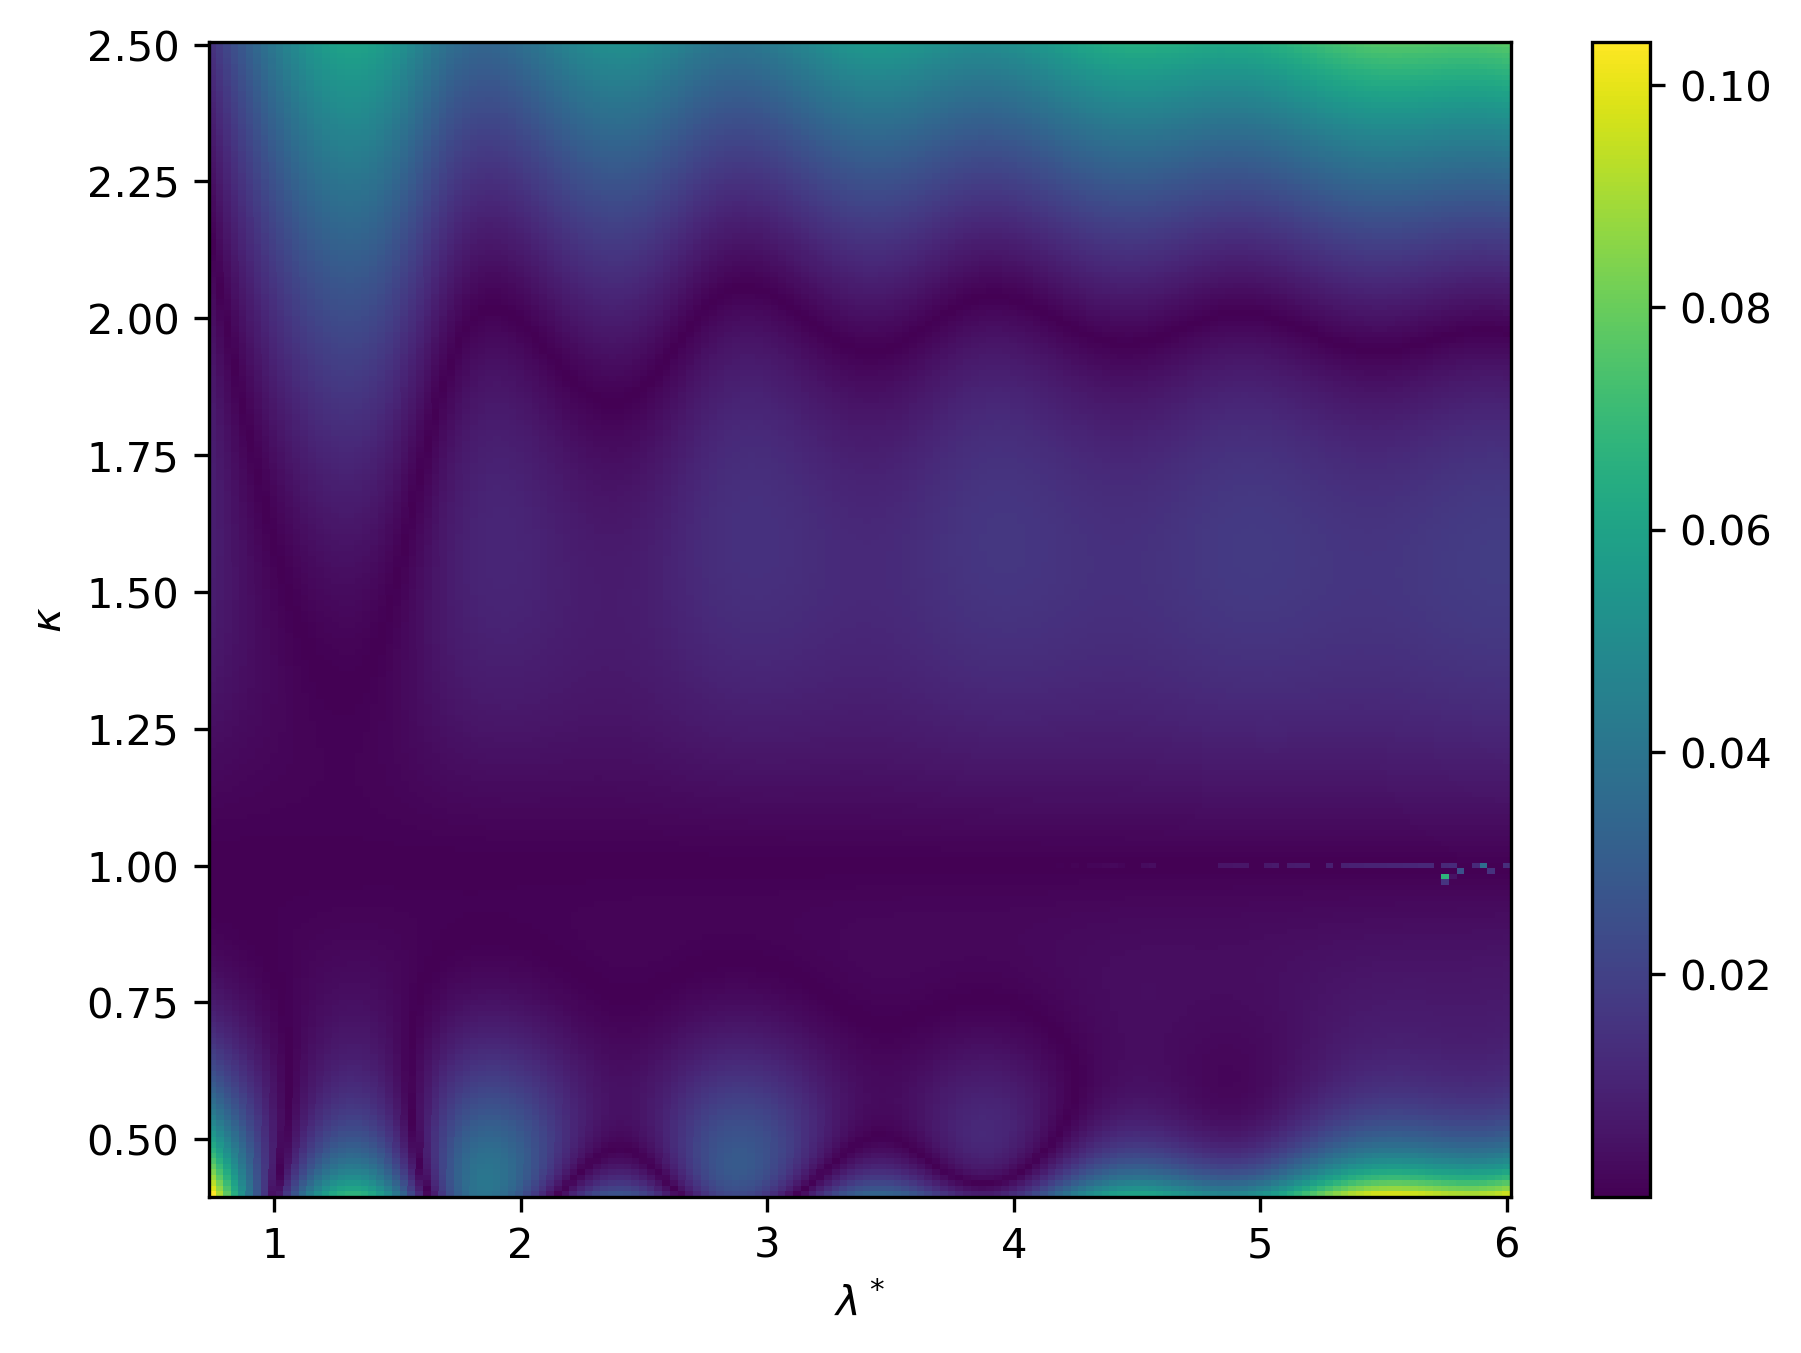
\includegraphics[width=\linewidth]{images/main_phase_error_heatmap.png}
		\par\smallskip
		$\widehat{\Psi}$
	\end{minipage}
	
	\vspace{1em}
	
	\begin{minipage}{0.48\textwidth}
		\centering
		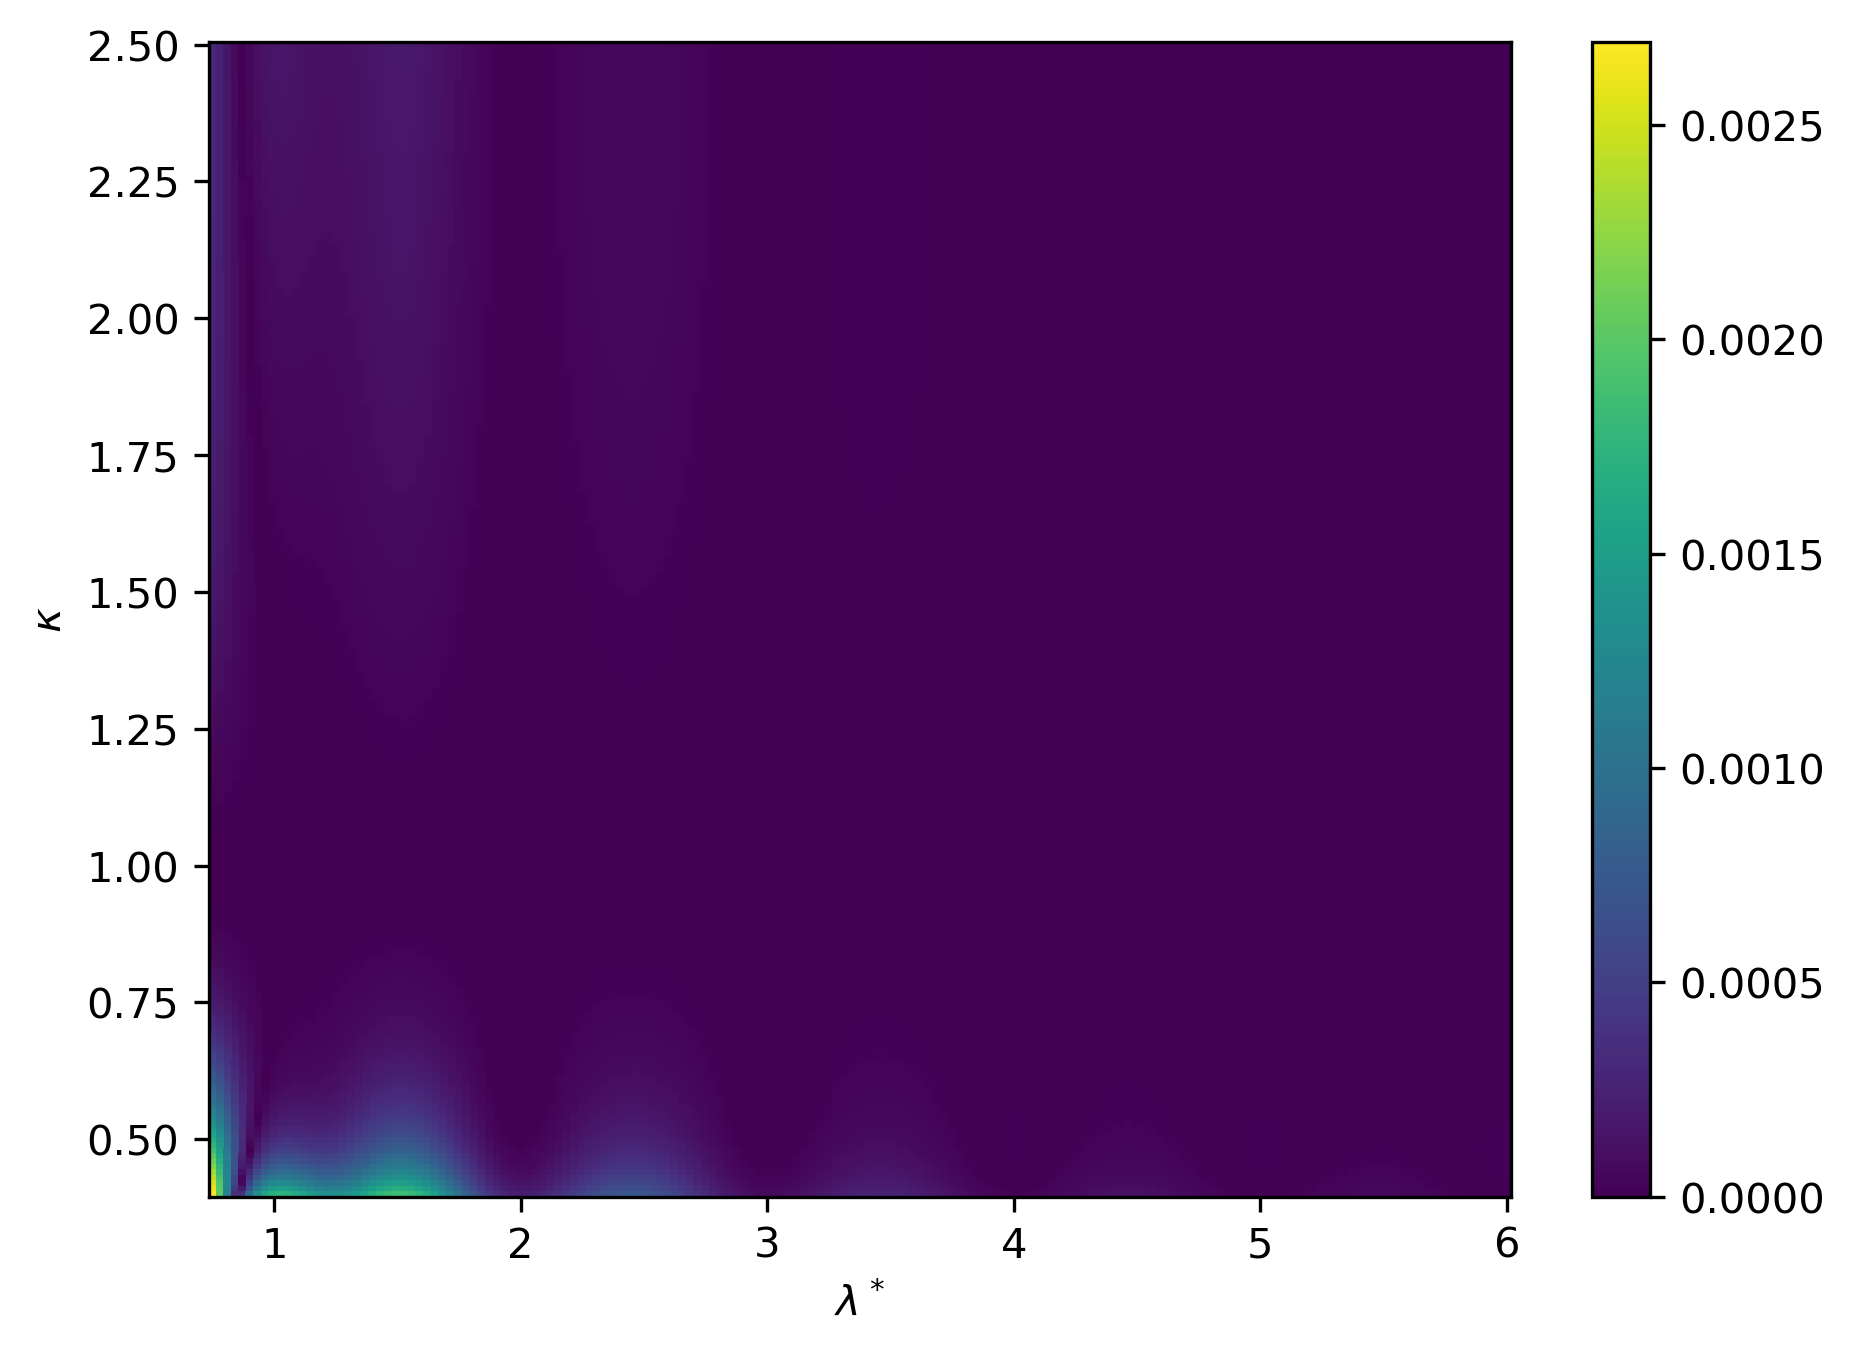
\includegraphics[width=\linewidth]{images/main_J_error_heatmap.png}
		\par\smallskip
		$\widehat{J}$
	\end{minipage}
	\hfill
	\begin{minipage}{0.48\textwidth}
		\centering
		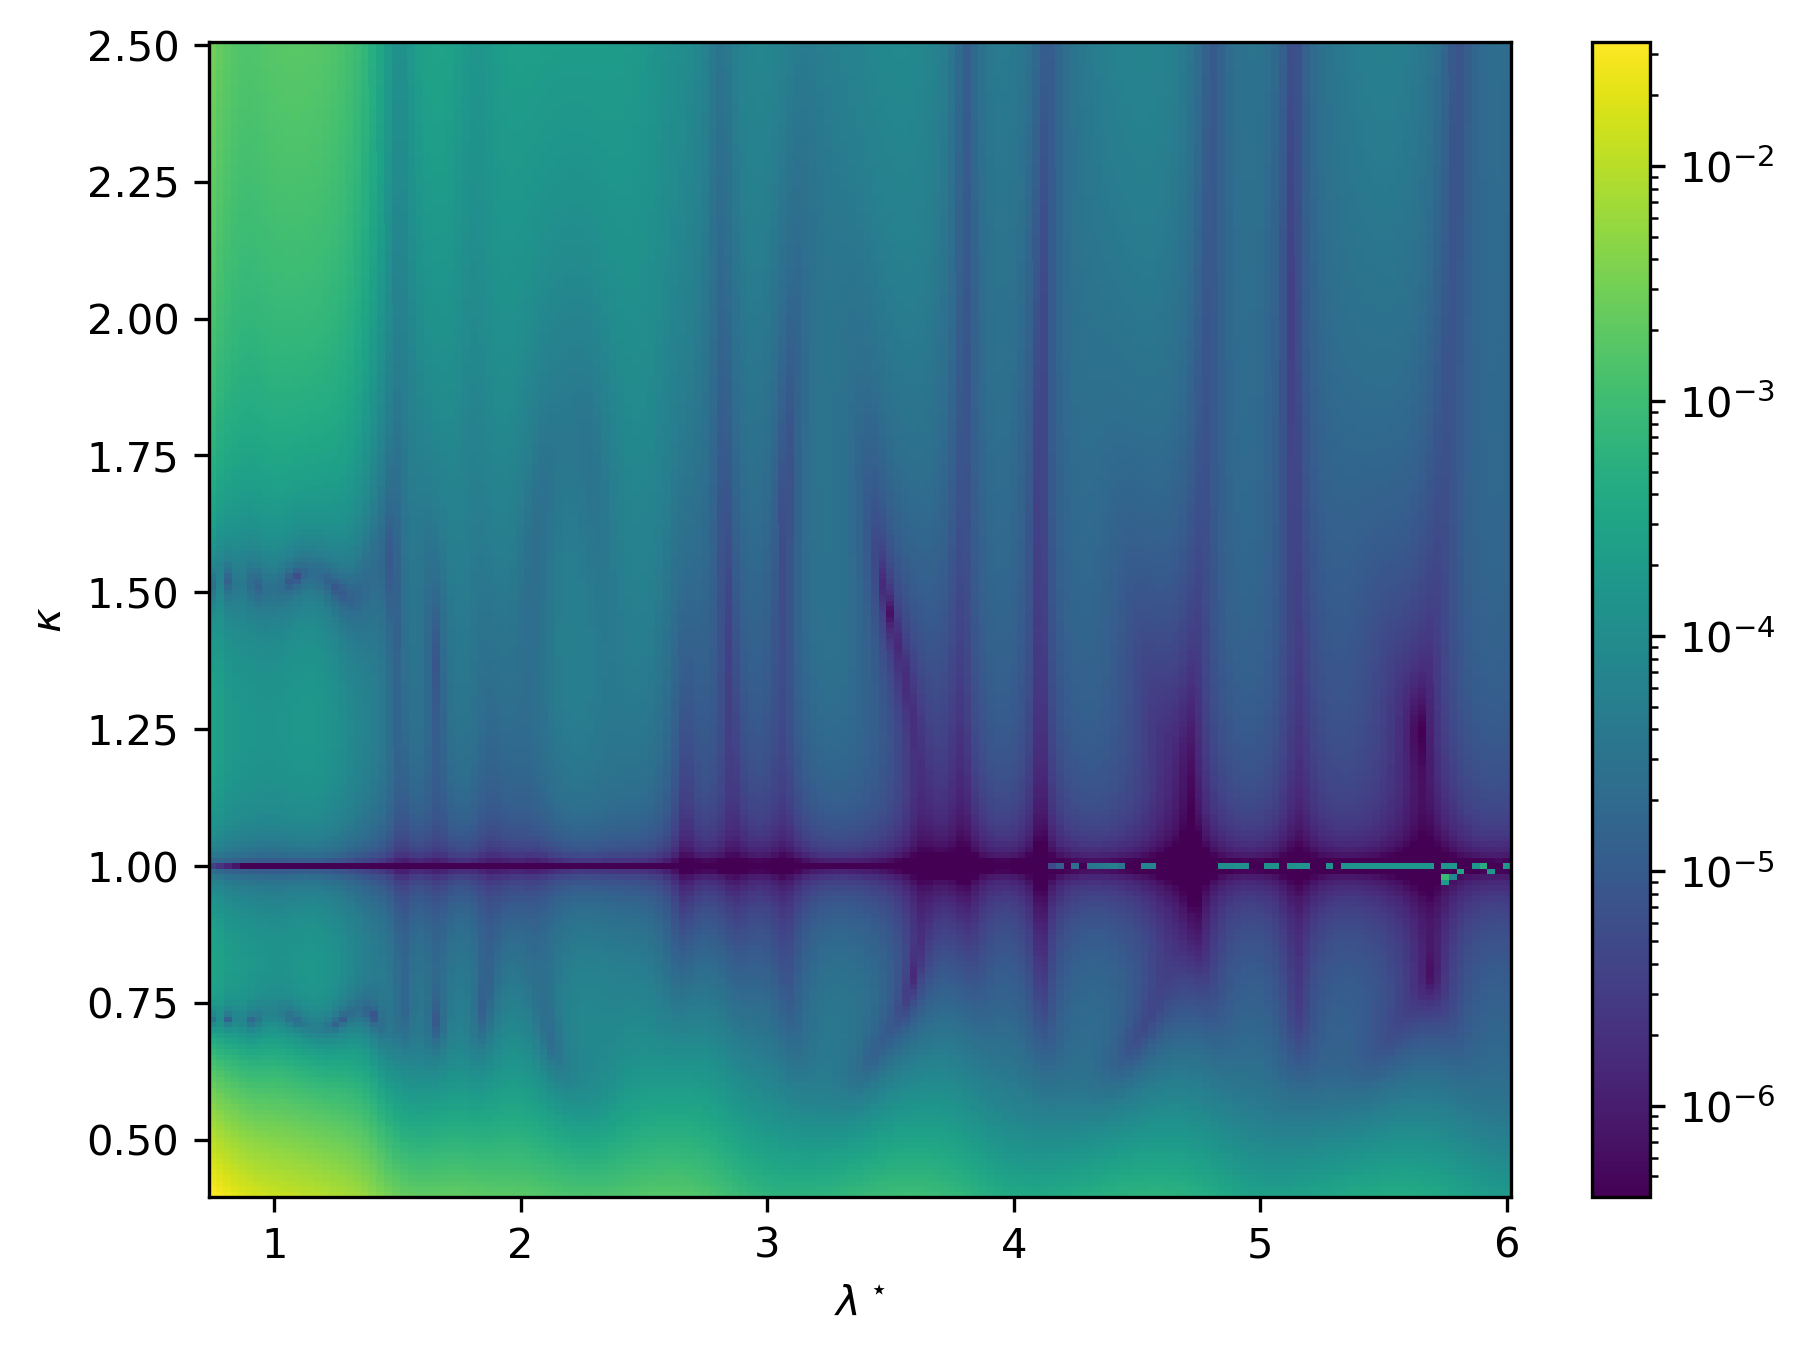
\includegraphics[width=\linewidth]{images/main_p_error_heatmap.png}
		\par\smallskip
		$\widehat{\mathbf z}_{0}$
	\end{minipage}
	
	\caption{Распределение ошибок конечных формул в основной области}
	\label{fig:chap2_main_error_heatmaps}
\end{figure}

Аналогичные метрики для области малой витковой дальности приведены в табл.~\ref{tab:chap2_short_metrics}. В этой области качество аппроксимаций в среднем ниже, что связано с менее регулярной структурой зависимостей. Тем не менее ошибки остаются достаточными для использования этих формул как технического расширения основного набора конечных формул.

\begin{table}[htbp]
	\centering
	\caption{Качество конечных формул в области малой витковой дальности}
	\label{tab:chap2_short_metrics}
	\begin{tabular}{l c c c c}
		\toprule
		Величина & Масштаб $S$ & RMSE $(\sigma)$ & MAE & $\max |e|$ \\
		\midrule
		$\widehat{T}_{\mathrm{short}}$ &
		$6.85480\cdot10^{-1}$ &
		$2.59570\cdot10^{-3}$ &
		$2.02066\cdot10^{-3}$ &
		$1.80235\cdot10^{-2}$ \\
		
		$\widehat{\Psi}_{T,\mathrm{short}}$ &
		$1.85044\cdot10^{-1}$ &
		$3.19594\cdot10^{-3}$ &
		$1.86307\cdot10^{-3}$ &
		$2.64622\cdot10^{-2}$ \\
		
		$\widehat{\Psi}_{\mathrm{short}}$ &
		$1.85044\cdot10^{-1}$ &
		$1.23122\cdot10^{-3}$ &
		$8.63699\cdot10^{-4}$ &
		$2.30663\cdot10^{-2}$ \\
		
		$\widehat{J}_{\mathrm{short}}$ &
		$2.48118\cdot10^{-1}$ &
		$3.19488\cdot10^{-3}$ &
		$1.38967\cdot10^{-3}$ &
		$4.24242\cdot10^{-2}$ \\
		
		$\widehat{p}_{rx,\mathrm{short}}$ &
		$9.97680\cdot10^{-1}$ &
		$1.40087\cdot10^{-2}$ &
		$7.97682\cdot10^{-3}$ &
		$2.59442\cdot10^{-1}$ \\
		
		$\widehat{p}_{ry,\mathrm{short}}$ &
		$7.14267\cdot10^{-1}$ &
		$2.14991\cdot10^{-2}$ &
		$1.34501\cdot10^{-2}$ &
		$2.23985\cdot10^{-1}$ \\
		
		$\widehat{p}_{vx,\mathrm{short}}$ &
		$5.15949\cdot10^{-1}$ &
		$5.86605\cdot10^{-3}$ &
		$3.52589\cdot10^{-3}$ &
		$5.58822\cdot10^{-2}$ \\
		
		$\widehat{p}_{vy,\mathrm{short}}$ &
		$3.95100\cdot10^{-1}$ &
		$1.45803\cdot10^{-2}$ &
		$9.55343\cdot10^{-3}$ &
		$2.03047\cdot10^{-1}$ \\
		
		$\widehat{\mathbf z}_{0,\mathrm{short}}$ &
		$1.38847$ &
		$3.00907\cdot10^{-2}$ &
		$2.12842\cdot10^{-2}$ &
		$2.65652\cdot10^{-1}$ \\
		\bottomrule
	\end{tabular}
\end{table}

Распределение ошибок в маловитковой области показано на рис.~\ref{fig:chap2_short_error_heatmaps}. В отличие от основной области, локальные зоны увеличенной ошибки занимают большую часть области параметров, что подтверждает вспомогательный характер соответствующих конечных формул.

\begin{figure}[htbp]
	\centering
	\begin{minipage}{0.48\textwidth}
		\centering
		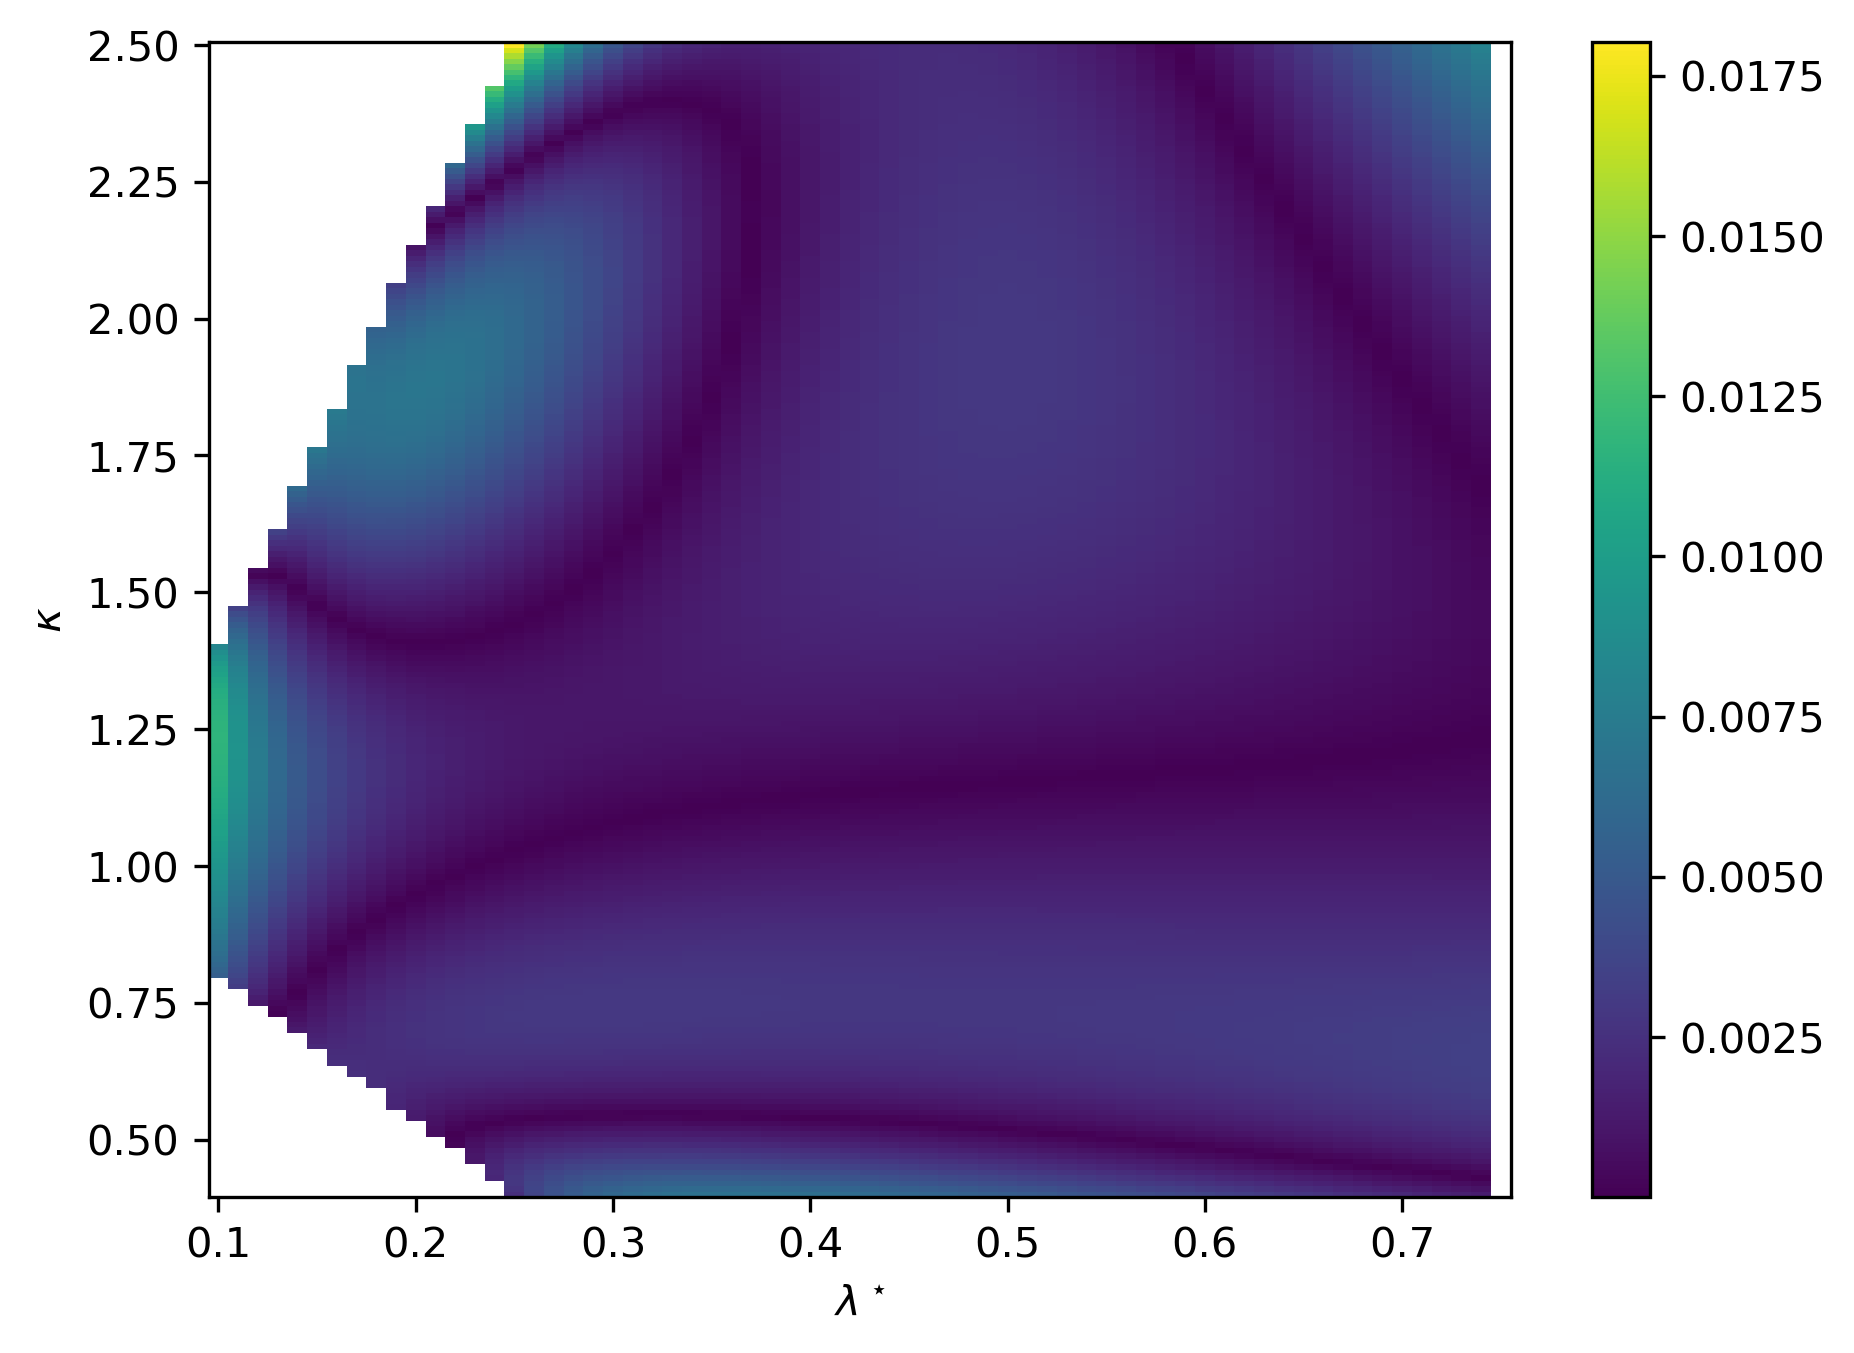
\includegraphics[width=\linewidth]{images/short_T_error_heatmap.png}
		\par\smallskip
		$\widehat{T}_{\mathrm{short}}$
	\end{minipage}
	\hfill
	\begin{minipage}{0.48\textwidth}
		\centering
		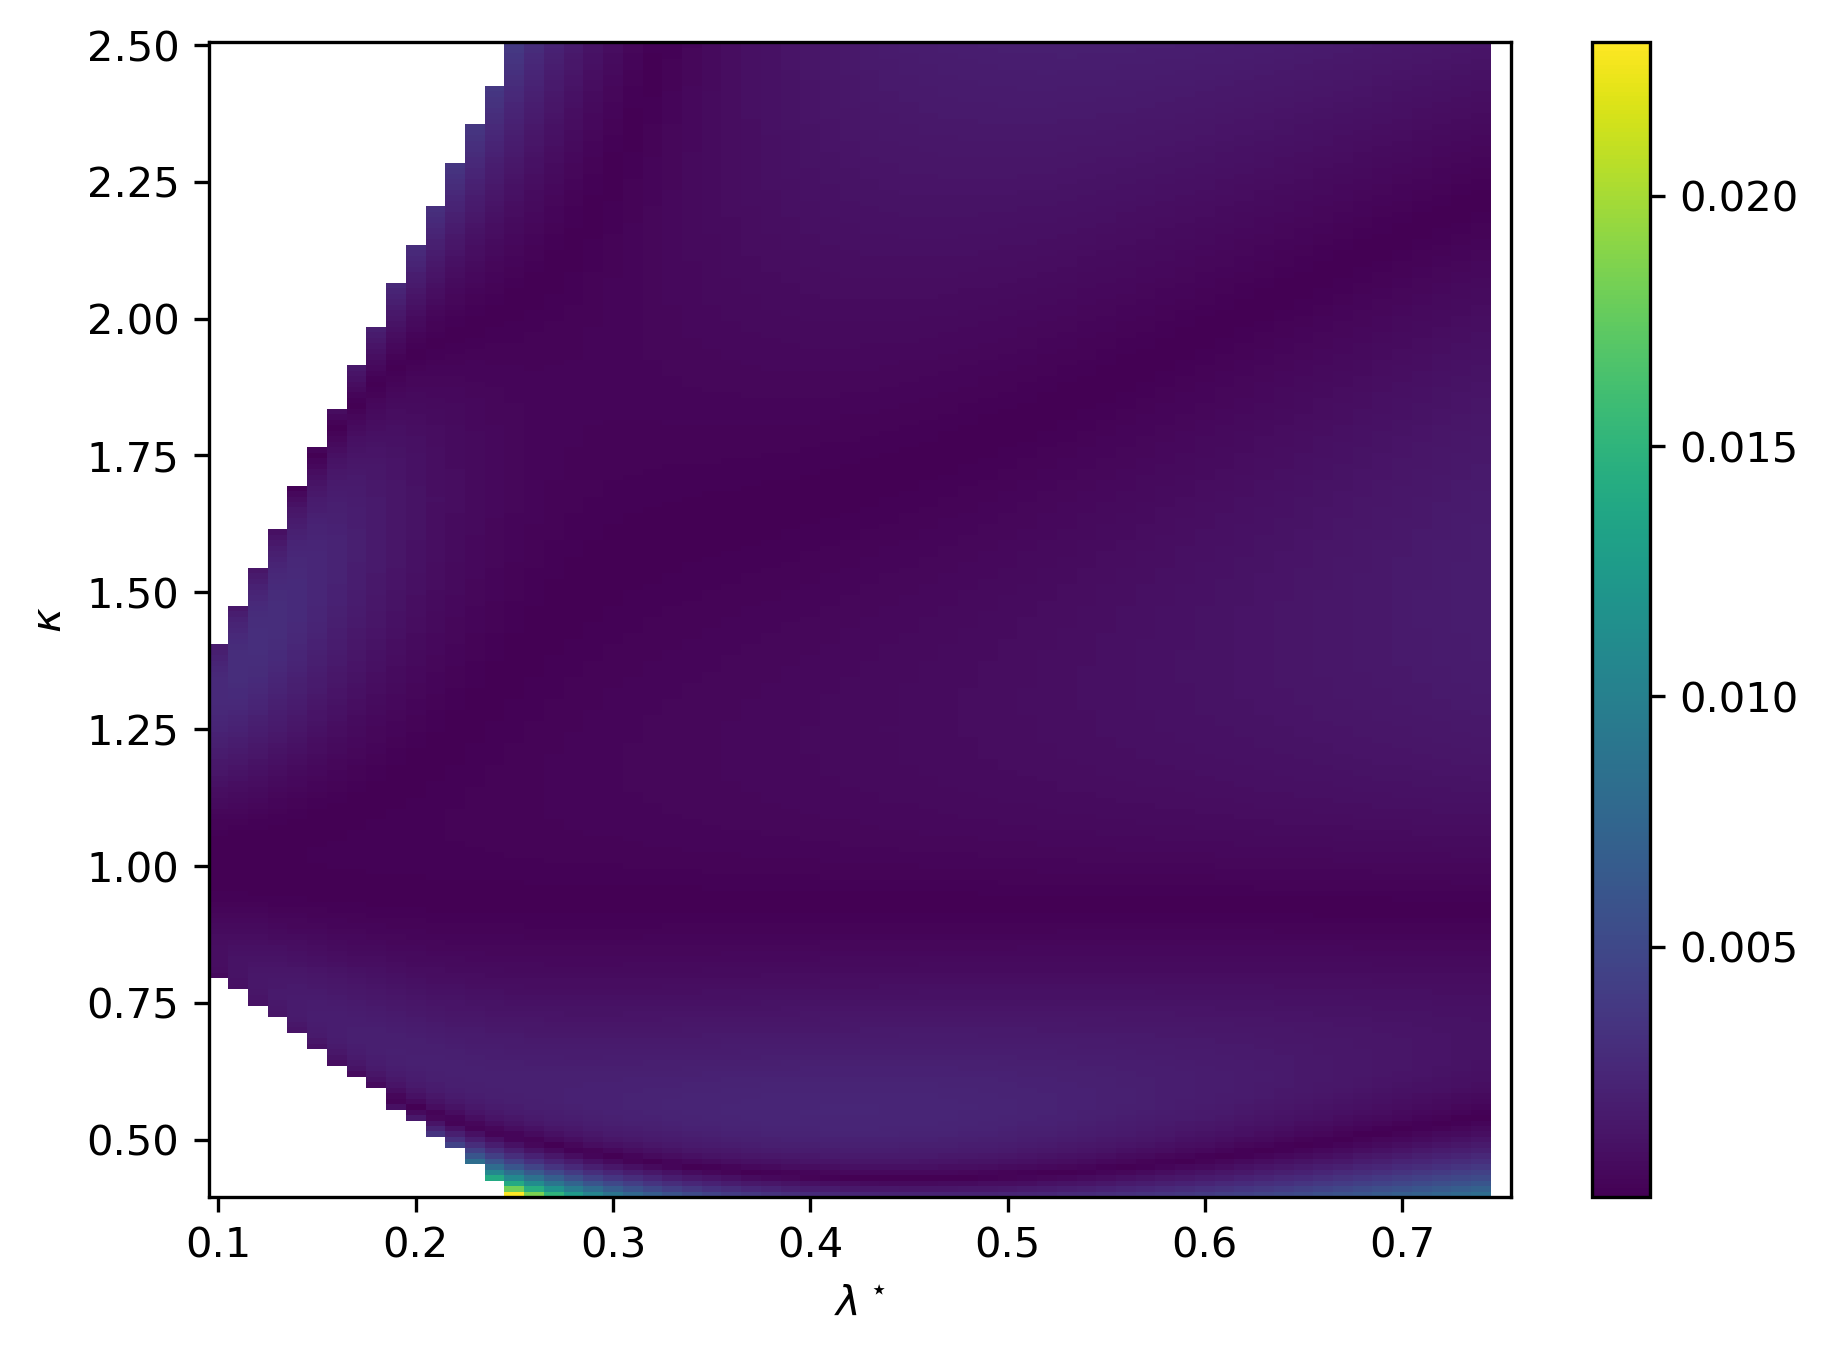
\includegraphics[width=\linewidth]{images/short_phase_error_heatmap.png}
		\par\smallskip
		$\widehat{\Psi}_{\mathrm{short}}$
	\end{minipage}
	
	\vspace{1em}
	
	\begin{minipage}{0.48\textwidth}
		\centering
		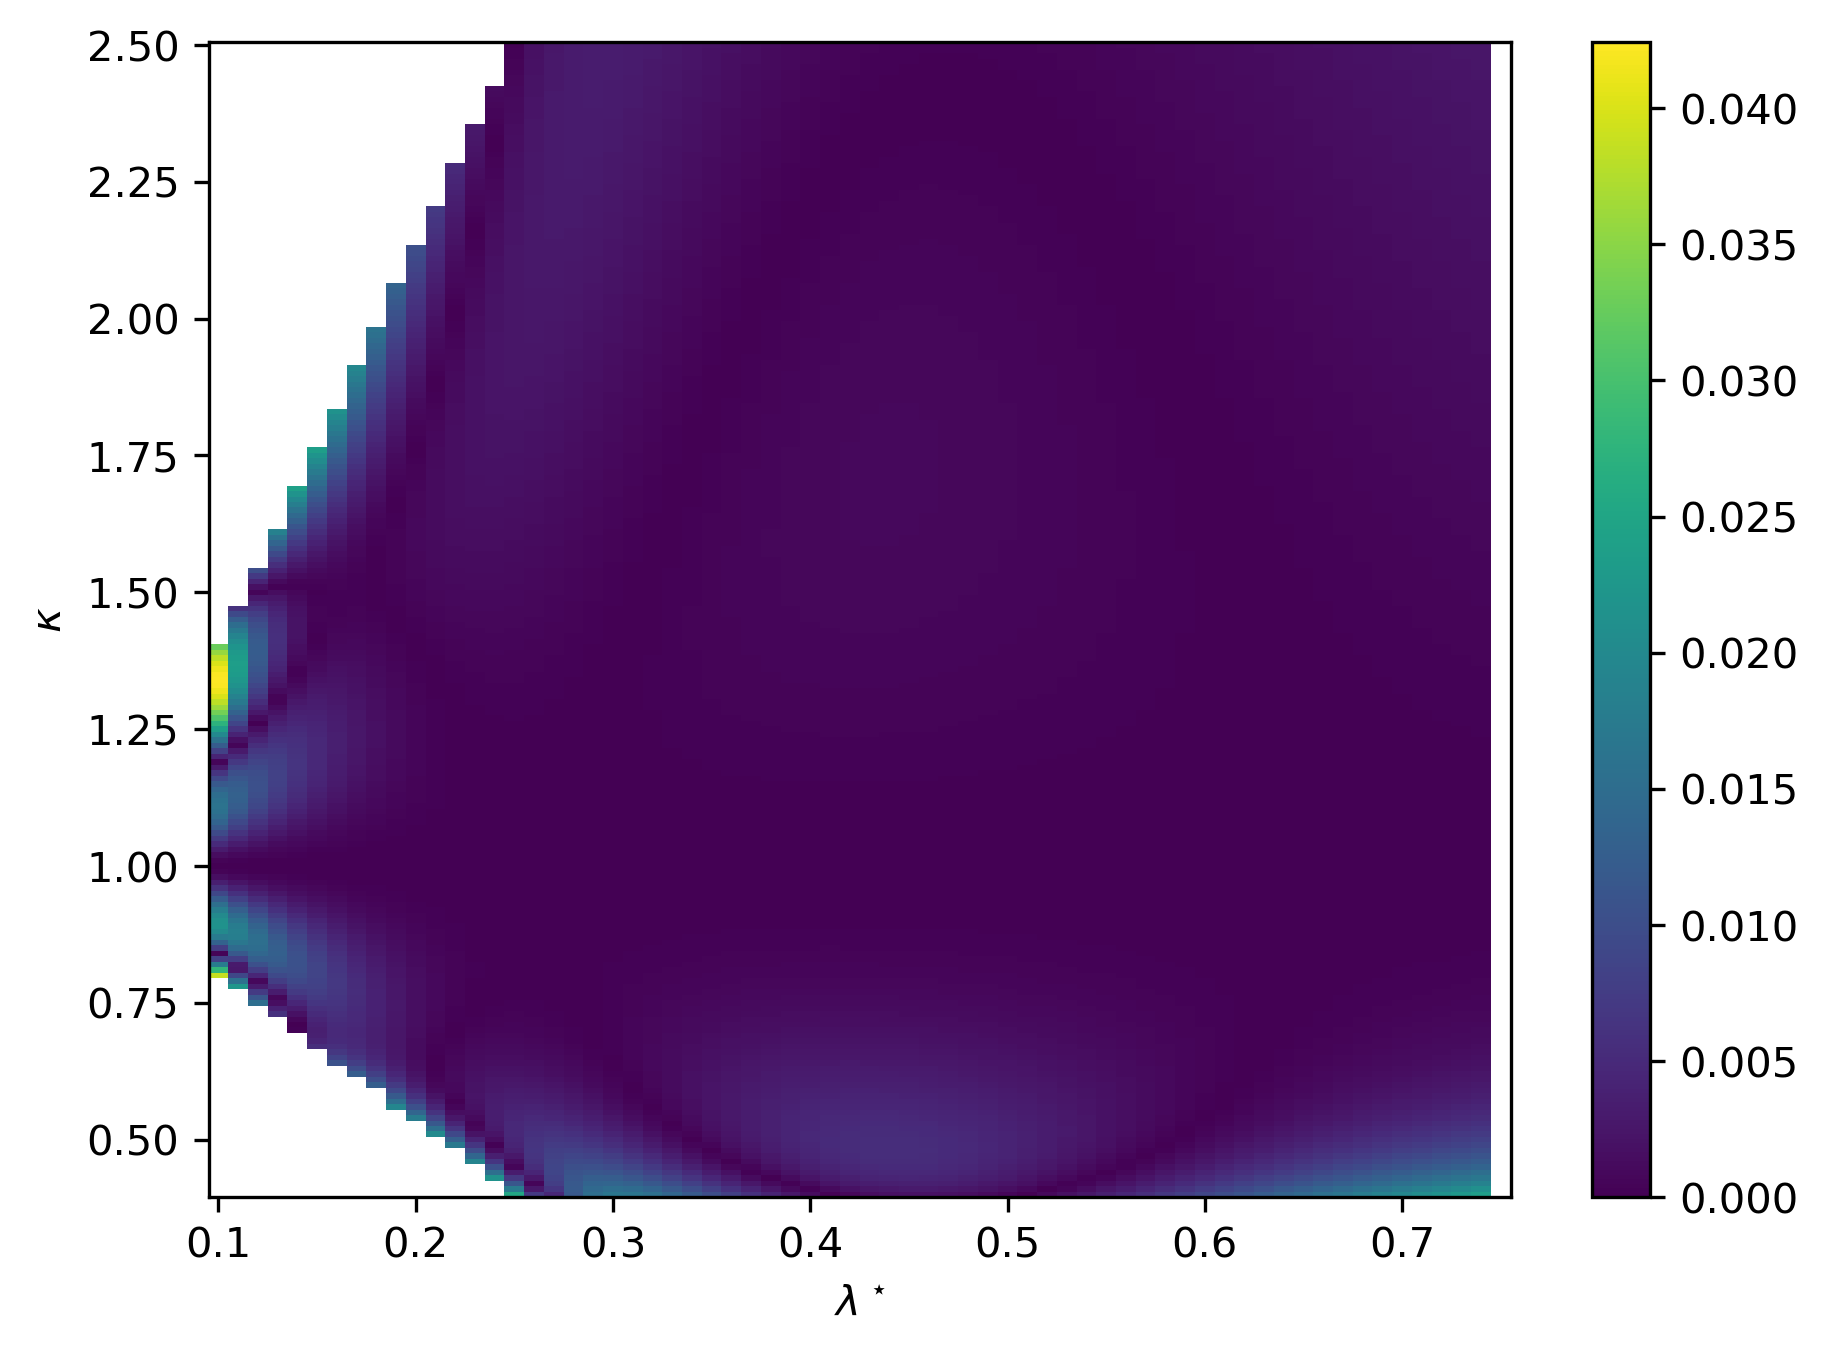
\includegraphics[width=\linewidth]{images/short_J_error_heatmap.png}
		\par\smallskip
		$\widehat{J}_{\mathrm{short}}$
	\end{minipage}
	\hfill
	\begin{minipage}{0.48\textwidth}
		\centering
		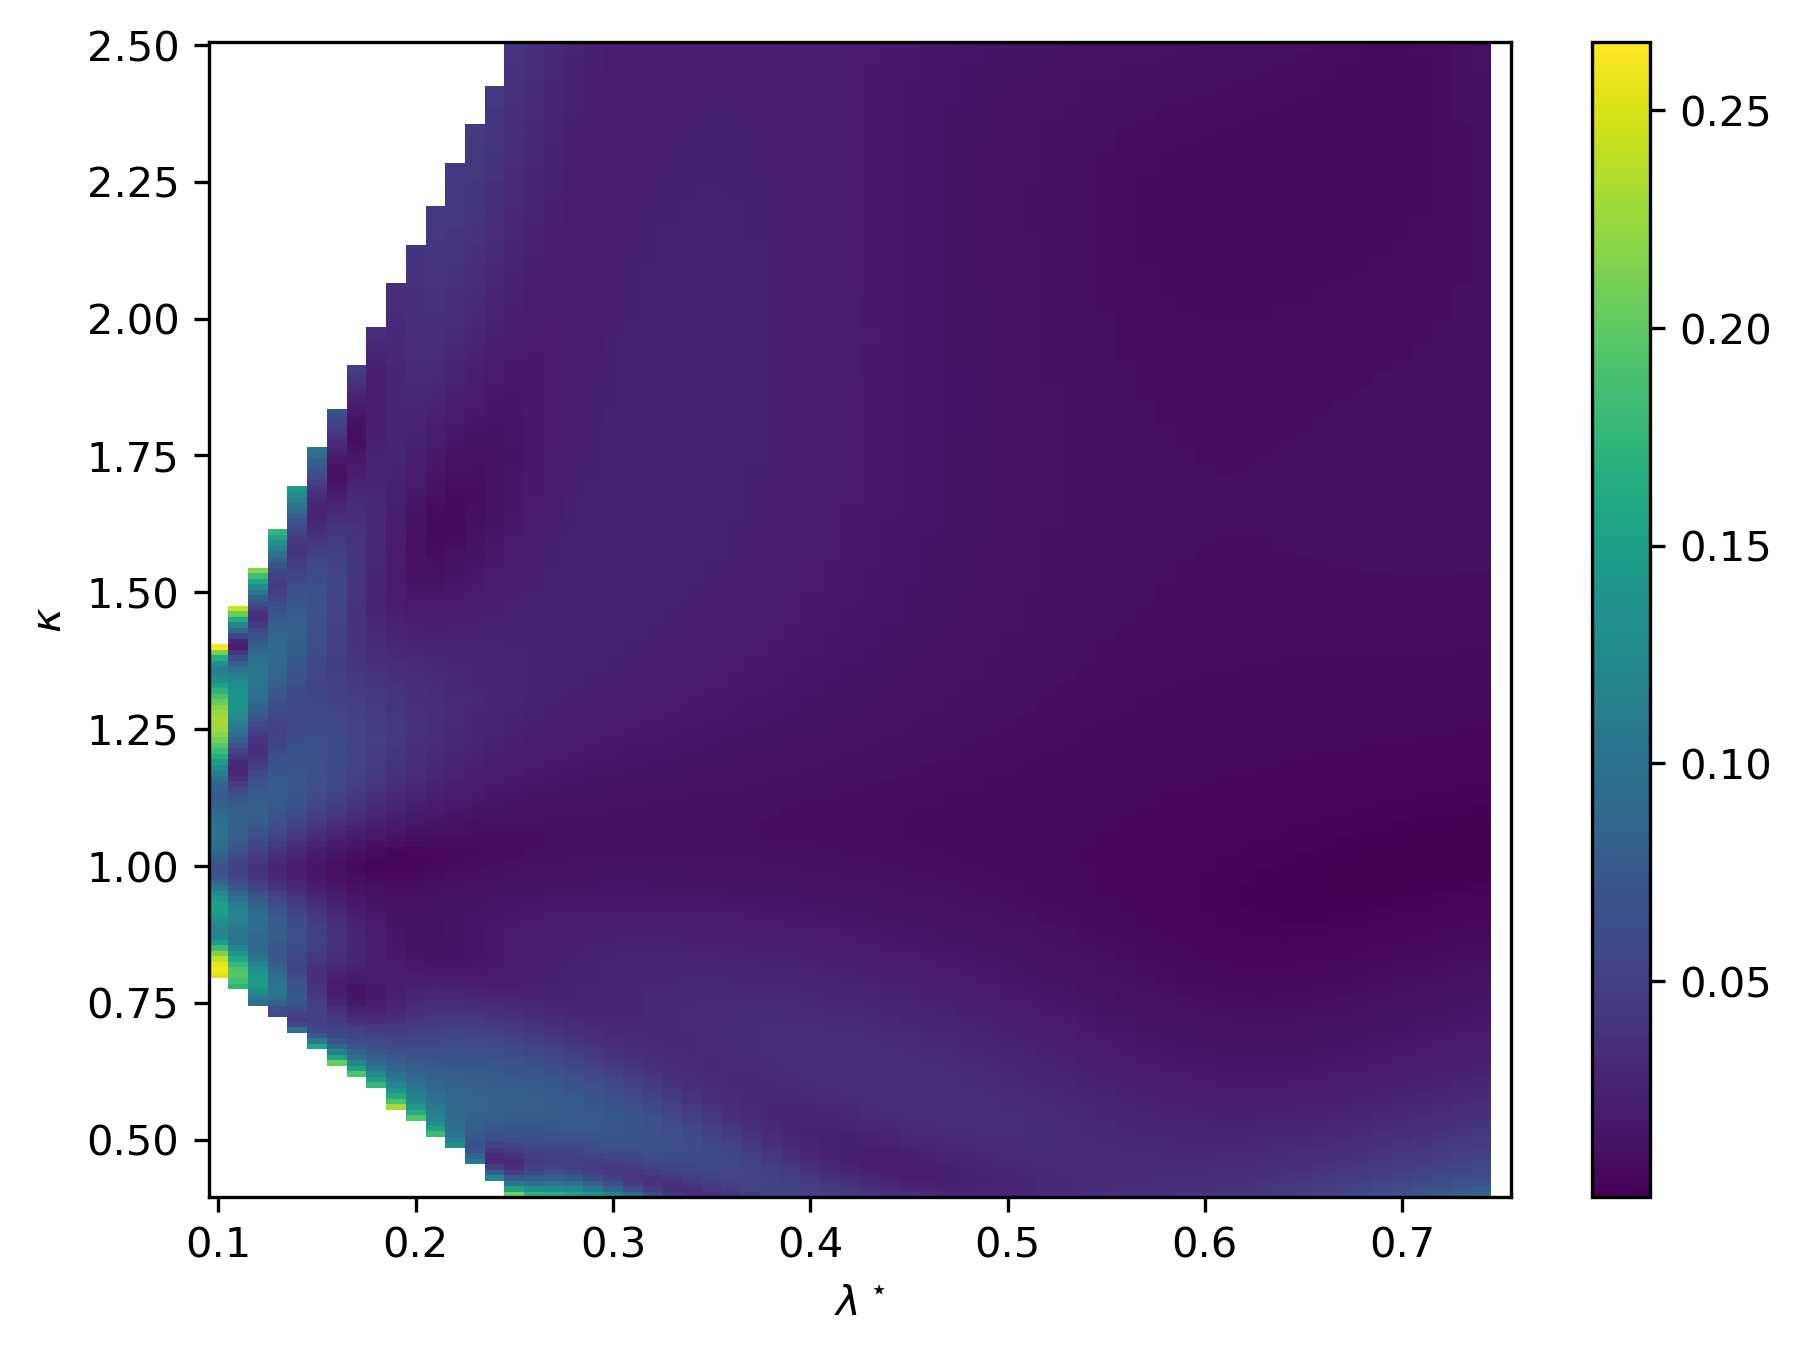
\includegraphics[width=\linewidth]{images/short_p_error_heatmap.png}
		\par\smallskip
		$\widehat{\mathbf z}_{0,\mathrm{short}}$
	\end{minipage}
	
	\caption{Распределение ошибок конечных формул в области малой витковой дальности}
	\label{fig:chap2_short_error_heatmaps}
\end{figure}

Отдельно сопоставим два способа задания нормированной непрерывной фазы. Первый способ использует кинематическую связь с продолжительностью перелёта и конечную формулу для $\widehat{T}$. Второй способ использует самостоятельную конечную формулу для $\widehat{\Psi}$. Как видно из табл.~\ref{tab:chap2_phase_compare}, во всех рассмотренных областях самостоятельная формула для непрерывной фазы даёт меньшую среднеквадратическую ошибку.

\begin{table}[htbp]
	\centering
	\caption{Сравнение способов задания нормированной непрерывной фазы}
	\label{tab:chap2_phase_compare}
	\begin{tabular}{l l c c c c}
		\toprule
		Область & Способ & Масштаб $S$ & RMSE $(\sigma)$ & MAE & $\max |e|$ \\
		\midrule
		Основная &
		$\widehat{\Psi}_{T}$ &
		$1.40529$ &
		$4.02183\cdot10^{-2}$ &
		$1.62921\cdot10^{-2}$ &
		$3.54534\cdot10^{-1}$ \\
		
		Основная &
		$\widehat{\Psi}$ &
		$1.40529$ &
		$1.88208\cdot10^{-2}$ &
		$1.26730\cdot10^{-2}$ &
		$1.03851\cdot10^{-1}$ \\
		
		Малая витковая дальность &
		$\widehat{\Psi}_{T,\mathrm{short}}$ &
		$1.85044\cdot10^{-1}$ &
		$3.19594\cdot10^{-3}$ &
		$1.86307\cdot10^{-3}$ &
		$2.64622\cdot10^{-2}$ \\
		
		Малая витковая дальность &
		$\widehat{\Psi}_{\mathrm{short}}$ &
		$1.85044\cdot10^{-1}$ &
		$1.23122\cdot10^{-3}$ &
		$8.63699\cdot10^{-4}$ &
		$2.30663\cdot10^{-2}$ \\
		\bottomrule
	\end{tabular}
\end{table}

Помимо сравнения с численно рассчитанными значениями, была выполнена дополнительная проверка согласованности конечных формул с краевыми условиями. Для этого по конечным формулам восстанавливались продолжительность перелёта и параметры оптимального управления, после чего выполнялось интегрирование уравнений движения. В конечный момент времени вычислялись невязки положения и скорости относительно целевой круговой орбиты.

На рис.~\ref{fig:chap2_main_terminal_residuals} показаны невязки правого конца для основной области. Эти карты характеризуют не отдельную ошибку аппроксимации одной величины, а совокупное качество восстановленного начального приближения.

\begin{figure}[htbp]
	\centering
	\begin{minipage}{0.48\textwidth}
		\centering
		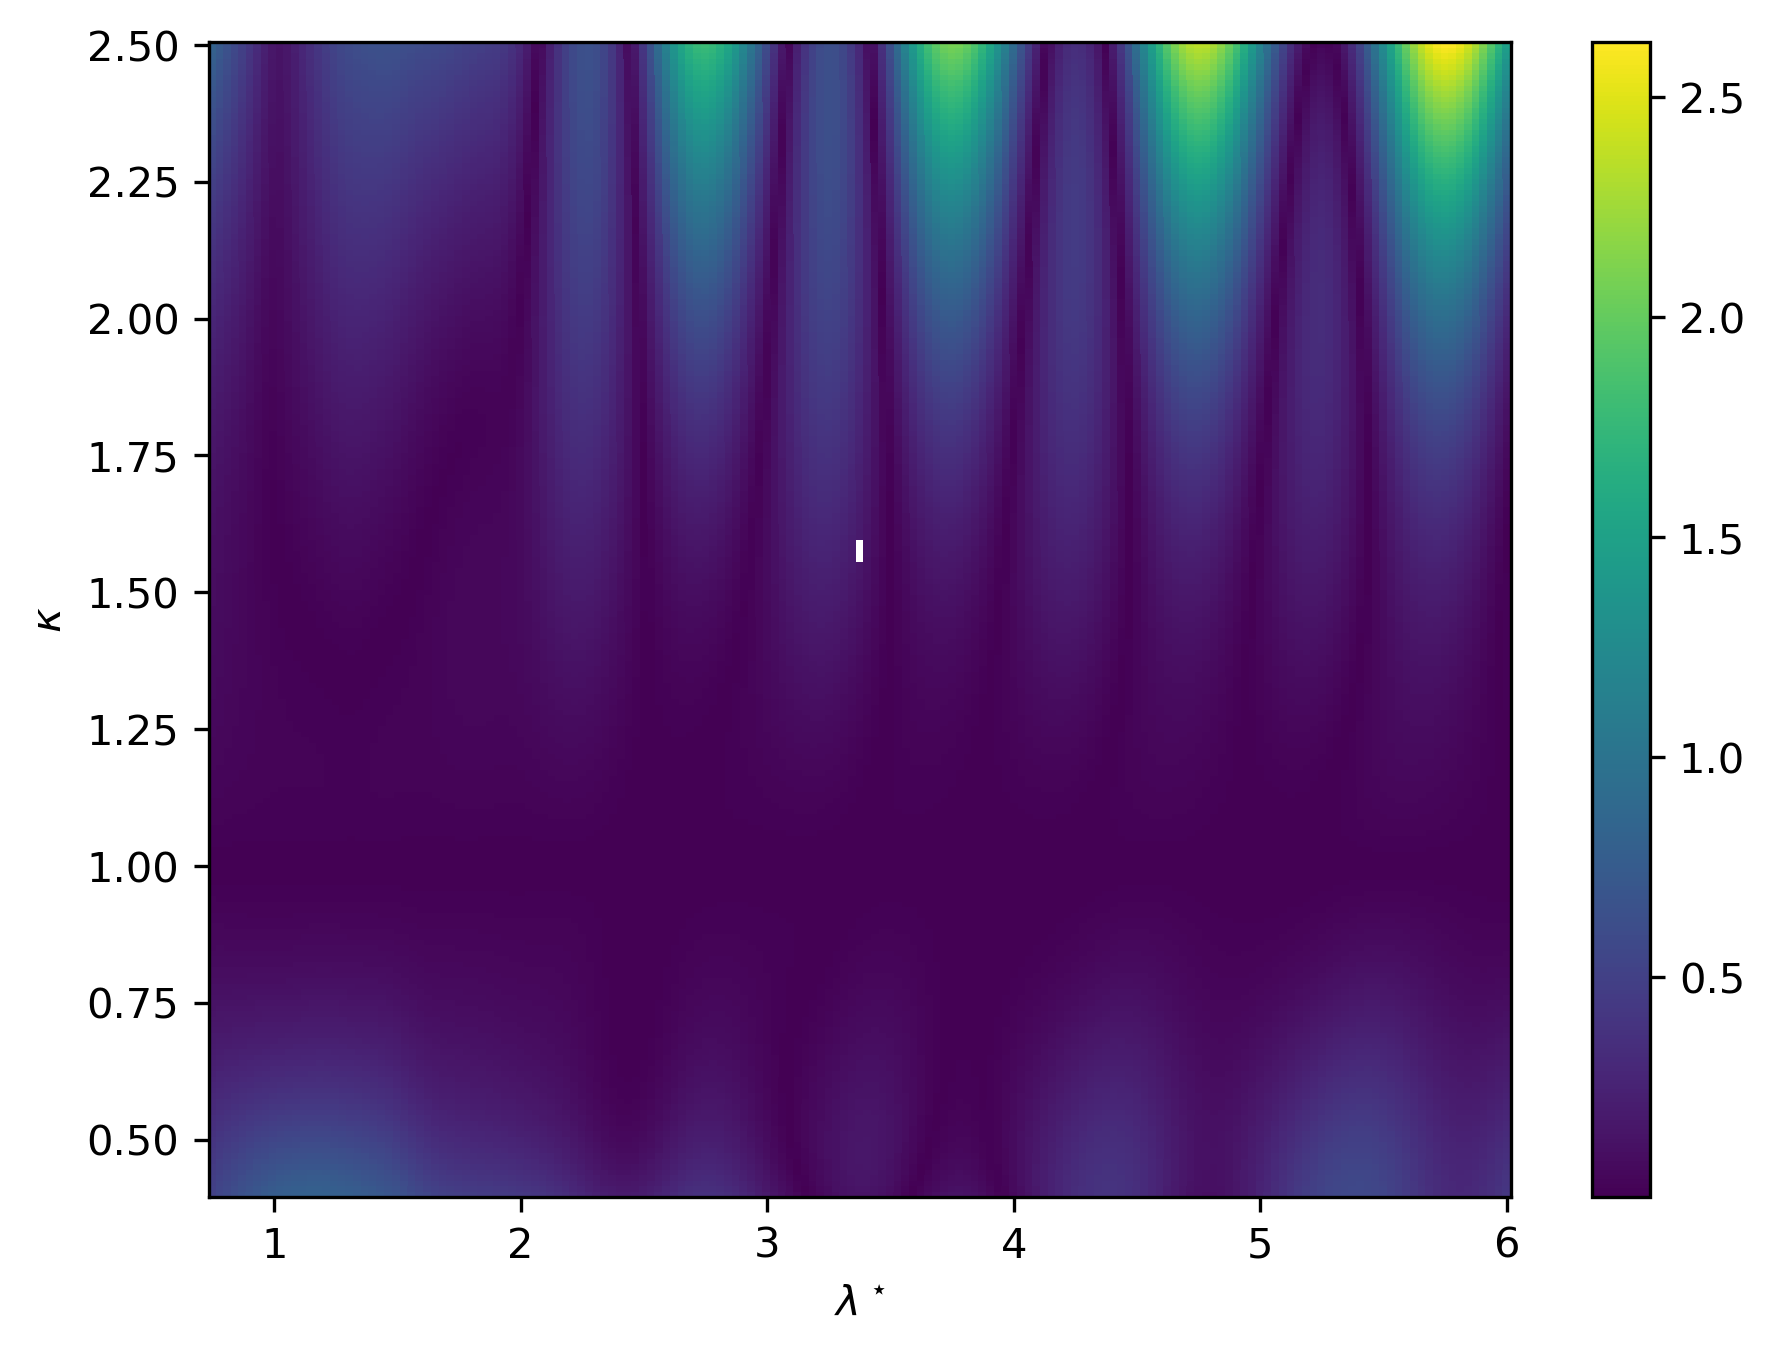
\includegraphics[width=\linewidth]{images/main_r_terminal_residual_heatmap.png}
		\par\smallskip
		Невязка положения
	\end{minipage}
	\hfill
	\begin{minipage}{0.48\textwidth}
		\centering
		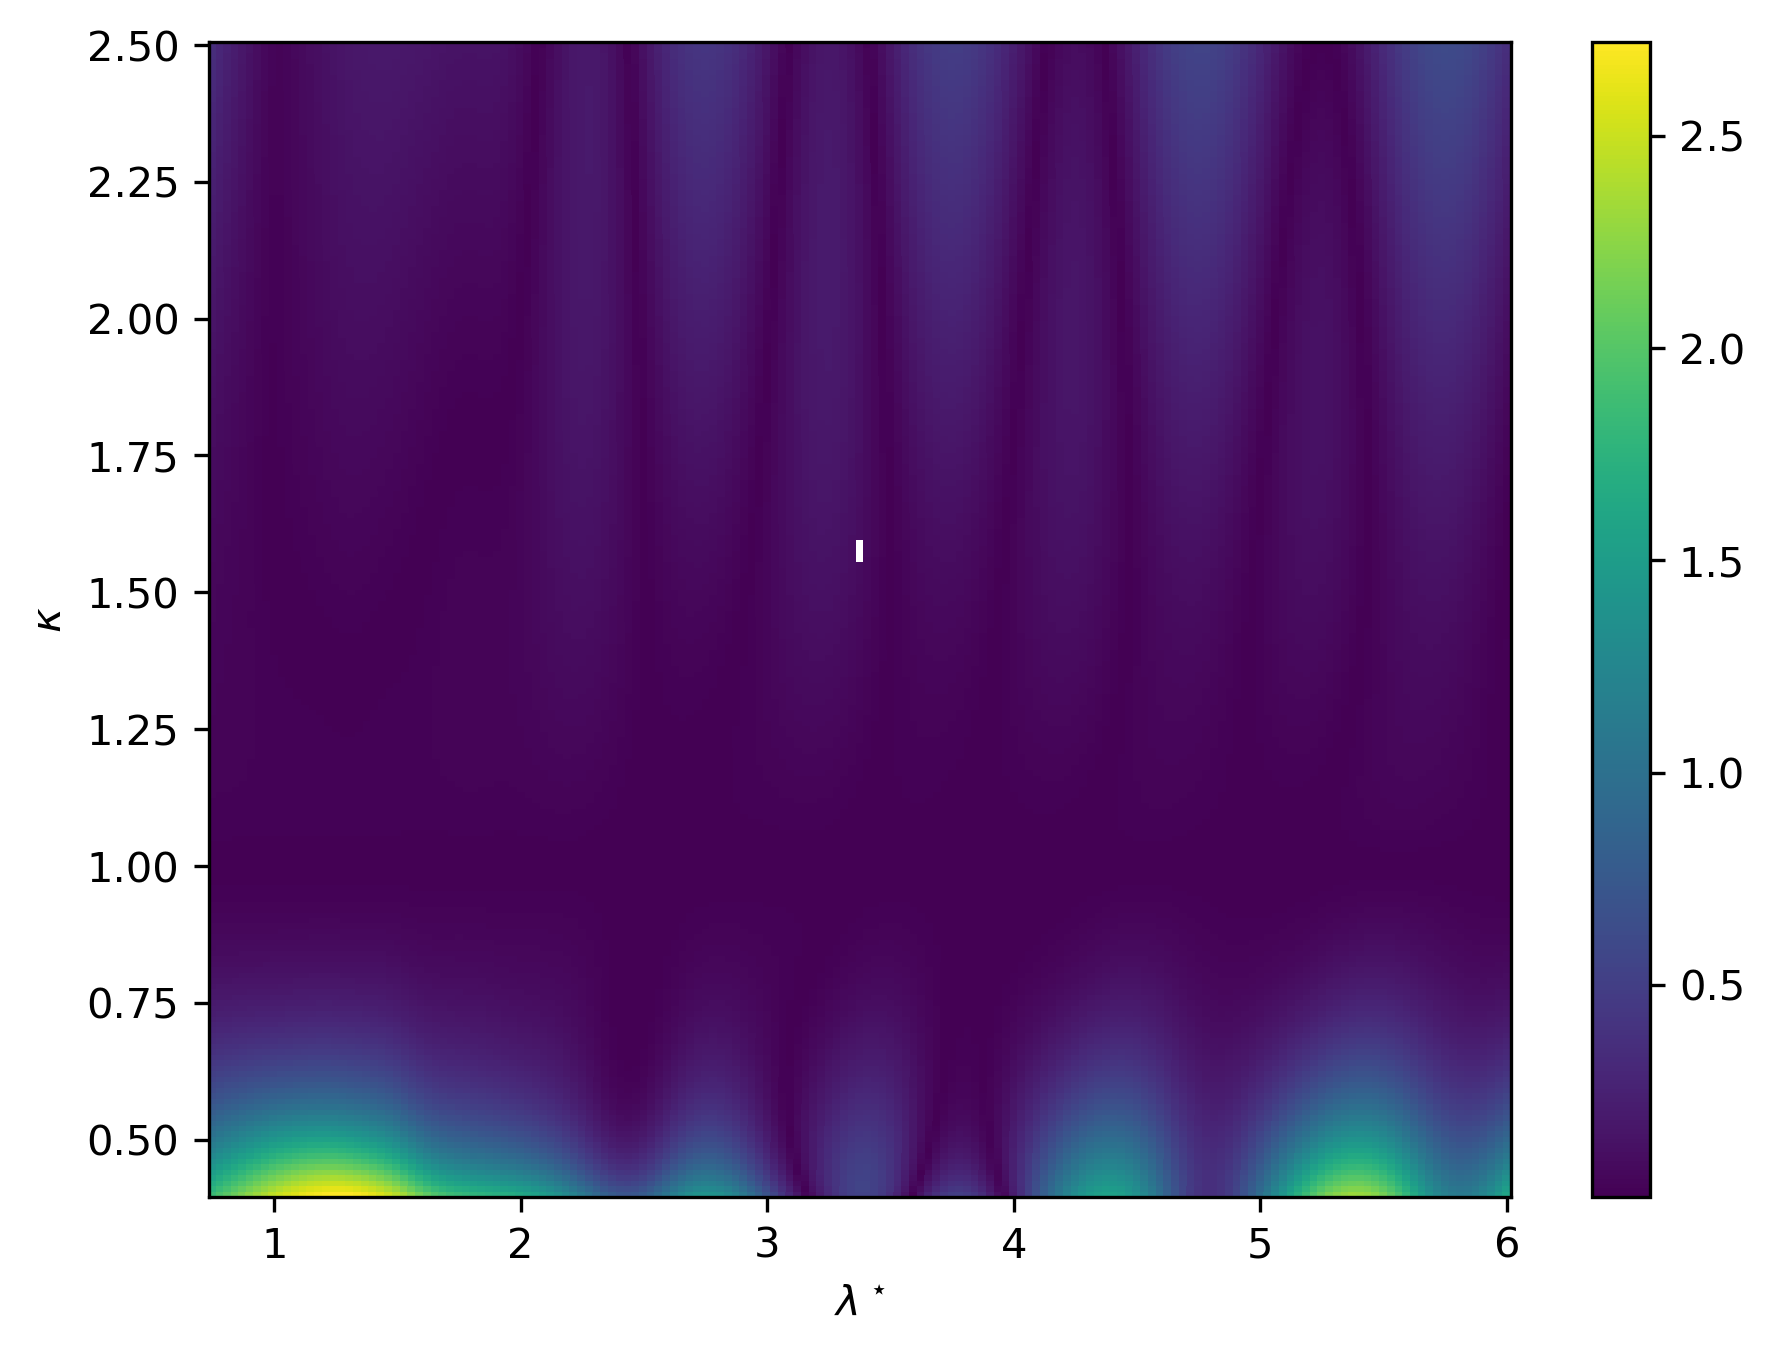
\includegraphics[width=\linewidth]{images/main_v_terminal_residual_heatmap.png}
		\par\smallskip
		Невязка скорости
	\end{minipage}
	\caption{Невязки правого конца при использовании конечных формул в основной области}
	\label{fig:chap2_main_terminal_residuals}
\end{figure}

Аналогичная проверка для области малой витковой дальности приведена на рис.~\ref{fig:chap2_short_terminal_residuals}. В этой области невязки выше, что согласуется с результатами табл.~\ref{tab:chap2_short_metrics}. Однако полученные значения остаются приемлемыми для роли маловиткового блока как вспомогательного участка при построении начального приближения.

\begin{figure}[htbp]
	\centering
	\begin{minipage}{0.48\textwidth}
		\centering
		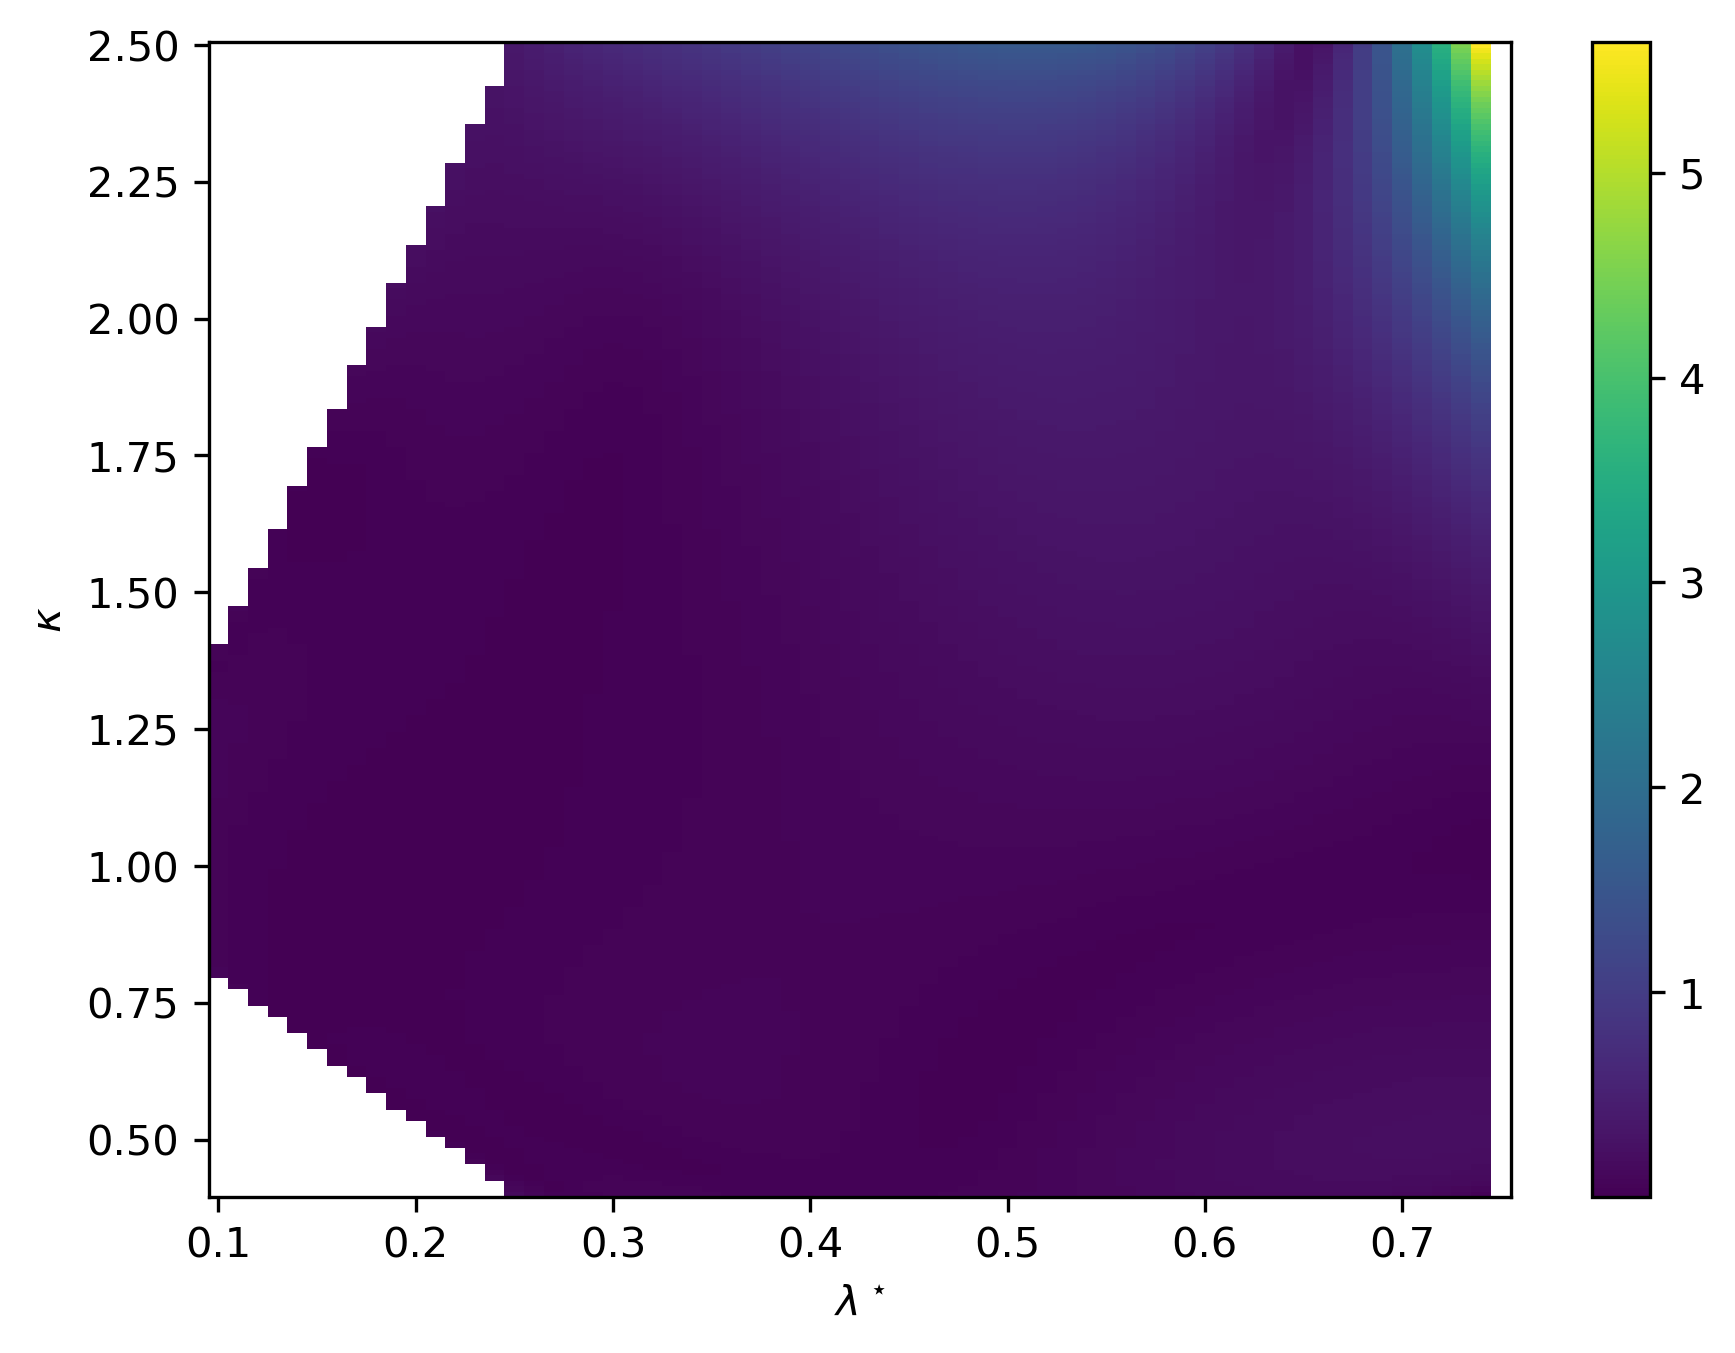
\includegraphics[width=\linewidth]{images/short_r_terminal_residual_heatmap.png}
		\par\smallskip
		Невязка положения
	\end{minipage}
	\hfill
	\begin{minipage}{0.48\textwidth}
		\centering
		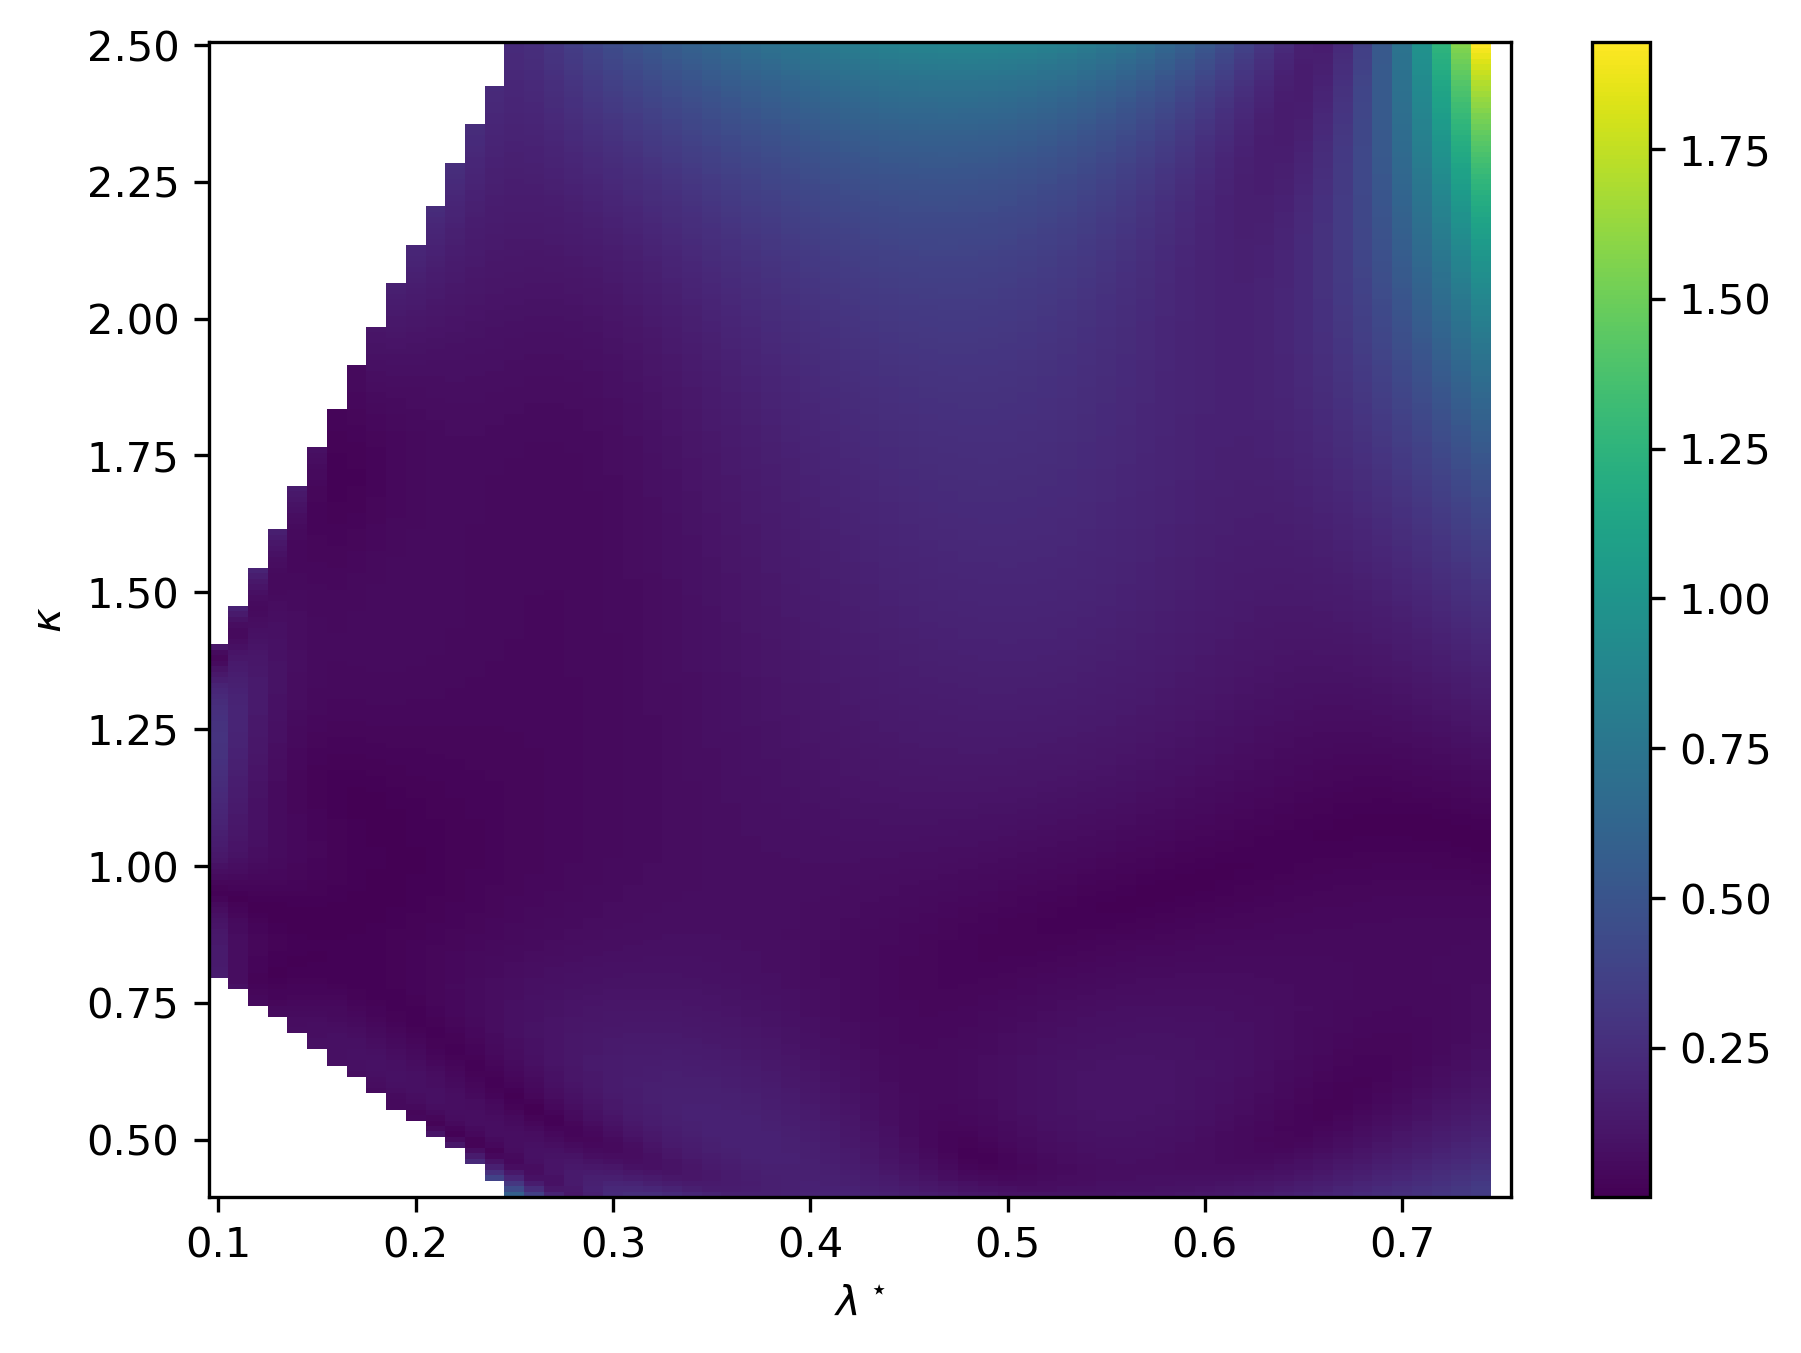
\includegraphics[width=\linewidth]{images/short_v_terminal_residual_heatmap.png}
		\par\smallskip
		Невязка скорости
	\end{minipage}
	\caption{Невязки правого конца при использовании конечных формул в области малой витковой дальности}
	\label{fig:chap2_short_terminal_residuals}
\end{figure}

Таким образом, построенные конечные формулы дают компактное приближённое описание кривых локальных оптимумов на рассматриваемой области параметров. Основная область описывается более точно и используется как главный рабочий диапазон. Область малой витковой дальности имеет более низкое качество аппроксимации, но обеспечивает устойчивость приближённого описания при переходе через малые значения $\lambda^\star$. Полученные оценки точности позволяют использовать конечные формулы как источник начального приближения для последующих задач оптимизации.


\section*{Выводы к главе 2}

Во второй главе исследована структура энергетически оптимальных решений в плоской круговой модели движения небесных тел. Полученные результаты показывают, что переход от эфемеридной постановки к модельной задаче позволяет выделить регулярную геометрическую структуру решений и построить для неё компактные конечные формулы, пригодные для дальнейшего использования при формировании начальных приближений.

\begin{enumerate}
	\item На примере перелётов Земля--Марс в эфемеридной постановке показано, что множество энергетически оптимальных решений имеет многоветвистую структуру. Эта структура служит исходной мотивацией для перехода к упрощённой плоской круговой модели, в которой дата старта заменяется начальной синодической фазой, а реальные планеты --- виртуальными небесными телами.
	
	\item Показано, что после устранения эфемеридной зависимости наблюдаемая многоветвистая структура переходит в односвязное модельное многообразие. В отдельных координатных представлениях это многообразие может визуально распадаться на ветви или самопересекаться, однако такой распад является свойством выбранного представления, а не самостоятельной структурой модельной задачи.
	
	\item Для модельного многообразия введена кривая локальных оптимумов. Она строится не отбором точек на заранее рассчитанной сетке, а как отдельная ветвь решений при дополнительном условии на свободный правый конец согласно принципу максимума. Для описания этой кривой используется локально оптимальная витковая дальность $\lambda^\star$.
	
	\item Введены точки оптимальной дальности как счётное множество точек пересечения кривой локальных оптимумов с изолиниями фиксированной начальной синодической фазы. Для последующего построения конечных формул вместо разрывной синодической фазы используется нормированная непрерывная фаза $\Psi$, представляющая собой её развёртку по витковой дальности.
	
	\item Для основной области построены конечные формулы для продолжительности перелёта $\widehat{T}$, нормированной непрерывной фазы $\widehat{\Psi}$, квадратичного функционала $\widehat{J}$ и параметров оптимального управления $\widehat{\mathbf z}_0$. Для непрерывной фазы также рассмотрено восстановление через кинематическую связь с продолжительностью перелёта; последующее сравнение показало преимущество самостоятельной конечной формулы для $\widehat{\Psi}$.
	
	\item Для параметров оптимального управления выявлена устойчивая попарная структура компонент начальных значений сопряжённых переменных. Конечные формулы включают основную часть с $C$-коэффициентами и быстро затухающие $D$-функции, которые описывают переходную область малой витковой дальности и позволяют сшить мало- и многовитковые решения в рамках одной записи.
	
	\item Для области малой витковой дальности построен отдельный набор конечных формул для скалярных характеристик и параметров оптимального управления. Эта область имеет более сложную структуру и более низкое качество аппроксимаций, однако её учёт необходим для устойчивого прохождения вычислительной процедуры через малые значения $\lambda^\star$.
	
	\item Выполнена верификация качества конечных формул в основной и маловитковой областях. Сравнение с численно рассчитанными значениями выполнено по характерному масштабу величины, среднеквадратической ошибке, средней абсолютной ошибке и максимальной абсолютной ошибке. Дополнительно проверены невязки правого конца после интегрирования уравнений движения с восстановленными продолжительностью перелёта и параметрами оптимального управления.
	
	\item Полученные конечные формулы задают компактное приближённое описание решений на кривых локальных оптимумов в координатах $\lambda^\star$ и $\kappa$. Эти зависимости будут использоваться далее как основа для переноса результатов на более общие постановки и для построения начального приближения в прикладных задачах баллистического проектирования.
\end{enumerate}